\documentclass[conference]{IEEEtran}
\IEEEoverridecommandlockouts
\usepackage{amsmath,amssymb,amsfonts}
\usepackage{algorithmic}
\usepackage{graphicx}
\usepackage{textcomp}
\usepackage{xcolor}
\usepackage{booktabs}
\usepackage{multirow}
\usepackage{url}
\usepackage[hidelinks]{hyperref}
\usepackage[utf8]{inputenc}
\providecommand{\lt}{<}
\ifdefined\DeclareUnicodeCharacter
\ifdefined\DeclareUnicodeCharacter
\ifdefined\DeclareUnicodeCharacter
  \DeclareUnicodeCharacter{2013}{\textendash}
  \DeclareUnicodeCharacter{2014}{\textemdash}
\fi
  \DeclareUnicodeCharacter{2014}{\textemdash}
\fi
  \DeclareUnicodeCharacter{2014}{\textemdash}
\fi

\def\BibTeX{{\rm B\kern-.05em{\sc i\kern-.025em b}\kern-.08em
    T\kern-.1667em\lower.7ex\hbox{E}\kern-.125emX}}

\begin{document}

\title{Preserved Accuracy, Restructured Logic: Attribution Drift and Output Saturation in INT8-Quantized Traffic Classifiers}

\author{\IEEEauthorblockN{Nur Nafis Fuad}
\IEEEauthorblockA{\textit{Department of Electrical and Computer Engineering} \\
\textit{Independent Researcher}\\
Jessore, Bangladesh \\
nnfuad01@gmail.com}
}

\maketitle

\begin{abstract}
Compressing deep neural network classifiers from 32-bit floating-point (FP32) to 8-bit integer (INT8) representations is standard practice for deploying encrypted traffic inspectors on resource-constrained edge hardware. Because post-quantization accuracy losses are typically small and negligible, often below one percentage point, practitioners assume the model's internal decision logic is preserved. We test that assumption directly. Using the ISCX VPN-NonVPN 2016 benchmark (339,009 bidirectional flows from 140 captures, partitioned into 106 leakage-free canonical session groups), we train a compact 1D Convolutional Neural Network (44,129 parameters) and compress it via both static Post-Training Quantization (PTQ) and Quantization Aware Training (QAT) under the PyTorch QNNPACK backend. We then apply KernelSHAP, a perturbation-based, model-agnostic attribution method compatible with discrete INT8 weights to 100 stratified test flows, benchmarking quantization-induced attribution drift against a multi-seed explainer noise floor. PTQ preserves dominant feature rankings almost exactly: 95 of 100 flows share identical Top-5 feature sets (Jaccard = 0.9786, signed cosine similarity = 0.9918). A paired Wilcoxon signed-rank test detects a small positive rank shift, but the median Total Variation displacement is only +0.0049. QAT tells a different story. Cosine similarity between FP32 and QAT attributions collapses to 0.4830 ($p < 10^{-17}$; vs. 0.9554 for an unquantized fine-tuning control), and unsigned 8-bit output quantization imposes a hard probability ceiling of 0.7338 that causes complete minority-class detection failure ($F_1 = 0.0000$ on the full 49,251-flow test set) when practitioners reuse the original decision threshold, recoverable only through explicit post-quantization calibration. Batched INT8 inference reaches 76--82 k flows/s which is 12 times over FP32; single-packet streaming yields only 1.05 times. These findings establish that predictive accuracy alone is an insufficient proxy for explainability fidelity after quantization.
\end{abstract}

\begin{IEEEkeywords}
Network traffic classification, Explainable AI (XAI), Neural network quantization, Model compression, Model calibration, KernelSHAP, Edge computing.
\end{IEEEkeywords}

\section{Introduction}
\IEEEPARstart{P}{ervasive} transport-layer encryption (TLS~1.3, QUIC, WireGuard) has fundamentally altered perimeter cybersecurity. By concealing packet payloads, encryption limits traditional deep packet inspection (DPI) to transport metadata, forcing Network Intrusion Detection Systems (NIDS) to rely on statistical features and packet timing dynamics~\cite{b1,b2,b3}. Deep representation learning has largely displaced manual feature engineering, using one-dimensional and two-dimensional convolutional networks (1D/2D-CNNs) and recurrent encoders to classify encrypted traffic directly from raw sequence headers.

Deploying automated classifiers into Security Operations Center (SOC) pipelines requires transparent, verifiable decision logic. High-confidence detections feed Security Orchestration, Automation, and Response (SOAR) playbooks, triggering automated endpoint isolation and dynamic Access Control List (ACL) drop rules. Operators must verify whether an alert stems from authentic protocol semantics or from spurious background artifacts such as ephemeral local port numbers. To verify decision boundaries against these artifacts, researchers have adopted post-hoc Explainable AI (XAI) frameworks, specifically cooperative game-theoretic Shapley values~\cite{b4}.

At the same time, real-time threat detection forces inference out of centralized cloud environments and onto physical perimeter hardware. Residential gateways, enterprise switches, and Customer Premises Equipment (CPE) must inspect traffic at line rate without introducing queuing jitter. Low-power ARM and MIPS edge cores operate under strict cache hierarchies where Level-1 data (L1-D) caches rarely exceed 32 to 64~KB per core. Storing full 32-bit floating-point (FP32) weights causes cache thrashing, high DRAM access latency, and memory bus saturation. Fixed-point integer quantization mitigates these hardware bottlenecks by mapping continuous 32-bit floating-point parameters to discrete 8-bit integers (INT8)~\cite{b5}. Under PyTorch QNNPACK, INT8 execution runs across 128-bit ARM NEON vector registers to compute sixteen 8-bit integer multiply-accumulate operations in parallel, shrinking model storage by up to 75\% and accelerating throughput.

Quantization typically follows two primary workflows~\cite{b5}:
\begin{enumerate}
    \item \textbf{Post-Training Quantization (PTQ):} A fast calibration step that maps pre-trained floating-point weights and activations to integer grids using scale and zero-point parameters.
    \item \textbf{Quantization-Aware Training (QAT):} A retraining scheme that models rounding and clipping during backpropagation using the Straight-Through Estimator (STE).
\end{enumerate}

To audit black-box classifiers, the cybersecurity community relies on post-hoc attribution methods, specifically KernelSHAP~\cite{b4}, which assigns additive importance values to input features. Practitioners operating edge inspection appliances operate under a critical operational assumption: because post-quantization accuracy and Macro $F_1$ drops are minimal (typically $< 1\%$), the model's internal decision logic is presumed to remain stable.

However, recent findings in computer vision and natural language processing show that model compression selectively damages rare data subpopulations and distorts internal representations even when top-line accuracy is preserved~\cite{b6}. In operational NIDS, logic corruption poses severe operational hazards:
\begin{enumerate}
    \item \textbf{Silent Logic Corruption:} Quantization can preserve classification labels while shifting feature importance onto spurious features, producing fragile edge classifiers vulnerable to evasion.
    \item \textbf{Brittle Defense Synthesis:} When automated SOAR engines ingest unverified attributions from quantized edge nodes to synthesize firewall rules, corrupted explanations generate flawed packet filters.
    \item \textbf{Regulatory and Compliance Exposure:} Governance frameworks (GDPR Article 22~\cite{b7}, the EU Artificial Intelligence Act~\cite{b8}, and NIST AI RMF 1.0~\cite{b9}) mandate transparency for automated systems affecting network access. Deploying unaudited compressed models introduces compliance risk.
\end{enumerate}

To address these challenges, this study formulates four fundamental research questions:
\begin{itemize}
    \item \textbf{RQ1 (Explainer Stochasticity):} What is the baseline stochastic noise floor of perturbation-based Shapley explainers on raw network packet sequences, and does static INT8-PTQ induce attribution displacement beyond this noise floor?
    \item \textbf{RQ2 (Quantization Algorithm Divergence):} How do PTQ and QAT differ in their impact on feature attribution geometry, ranking stability, and class-conditional attribution drift?
    \item \textbf{RQ3 (Causal Confounder Isolation):} Does attribution restructuring in QAT stem from discrete integer arithmetic, or does it reflect gradient descent optimization navigating an overparameterized loss surface?
    \item \textbf{RQ4 (Microarchitectural and Calibration Hazards):} What practical deployment hazards arise when running quantized classifiers on edge runtimes, and how does session grouping impact statistical confidence?
\end{itemize}

\begin{figure*}[htbp]
\centering
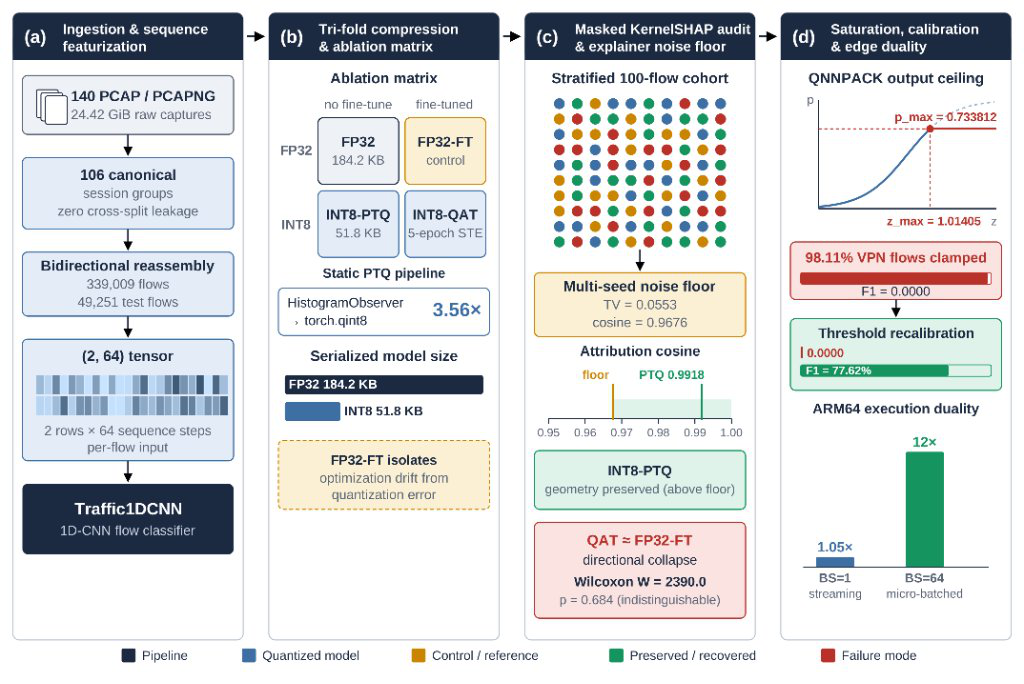
\includegraphics[width=\textwidth]{figures/figure1_conceptual_overview.png}
\caption{The XDrift Analytical Framework for Quantized Network Traffic Classifiers. (a) Bidirectional network flow ingestion, 106-session canonical isolation, and 2D sequence featurization. (b) 2 $\times$ 2 causal factorial matrix isolating integer quantization noise from stochastic fine-tuning drift. (c) Model-agnostic Masked KernelSHAP auditing across an $N = 100$ flow cohort evaluated against a multi-seed explainer noise floor boundary. (d) Operational consequences of affine dequantization: probability saturation ($p_{\max} = 0.733812$), classification blackout under default thresholds, recovery via threshold calibration, and microarchitectural edge latency duality on physical ARM64 hardware.}
\label{fig:conceptual_overview}
\end{figure*}

This paper delivers the following contributions:
\begin{enumerate}
    \item \textbf{First Quantitative Audit of Attribution Drift in Quantized NIDS:} We establish the empirical noise floor of KernelSHAP across multiple random seeds, demonstrating that static PTQ preserves Top-5 feature overlap with 95\% fidelity ($S_c = 0.9918$), while QAT induces severe directional collapse ($S_c = 0.4830$ overall, collapsing to $0.1665$ on minority VPN flows).
    \item \textbf{Causal Disentanglement of Quantization and Optimization Drift:} By introducing an unquantized fine-tuning baseline (FP32-FT), we demonstrate that fine-tuning accounts for initial representational migration across the loss surface, while integer constraints and STE approximations under QAT drive additional severe attribution collapse.
    \item \textbf{Discovery of the Quantized Output Probability Saturation Ceiling:} We identify a hardware-software deployment hazard where linear layer affine dequantization under PyTorch QNNPACK enforces an absolute upper bound of $p_{\max} = 0.733812$, causing a 100\% classification blackout on minority VPN flows under default operating thresholds.
    \item \textbf{Session-Clustered Statistical Inference Protocol:} We show that unclustered flow-level evaluations produce up to 56$\times$ standard error deflation, concealing Simpson's Paradox where a single massive capture session reverses the aggregate logit shift direction.
\end{enumerate}

The remainder of this paper is organized as follows: Section~II reviews related work. Section~III details the XDrift methodology and experimental design. Section~IV presents empirical results. Section~V discusses operational implications, threat models, regulatory compliance, and architectural rules. Section~VI concludes the paper.

\section{Related Work}

Early encrypted-traffic studies used flow-level statistics and conventional machine learning classifiers (such as decision trees and k-nearest neighbors) to distinguish VPN from non-VPN traffic and to characterize application categories~\cite{b1}. To eliminate manual feature engineering, subsequent research applied deep representation learning directly to packet datagrams. Wang et al. evaluated one-dimensional and two-dimensional convolutional networks on raw packet byte sequences for encrypted traffic and malware classification~\cite{b2}, while Lotfollahi et al. introduced Deep Packet, demonstrating that 1D-CNNs and stacked autoencoders achieve high precision on encrypted application and service identification~\cite{b3}. Subsequent studies extended packet modeling across diverse deep learning architectures: Aceto et al. designed MIMETIC, combining convolutional and recurrent neural layers to capture multimodal mobile traffic behaviors~\cite{b10}; Liu et al. developed FS-Net, modeling bidirectional flow sequences with recurrent encoders to capture long-range packet dependencies~\cite{b11}; van Ede et al. proposed FlowPrint, employing semi-supervised graph fingerprints to recognize encrypted mobile applications across network environments without labeled destination profiles~\cite{b12}; Lin et al. presented ET-BERT, adapting pre-trained transformers to learn contextualized representations from datagram bursts~\cite{b13}; and Chen and Wang designed MPAF, combining multi-phase attribute fingerprints extracted across connection lifecycles~\cite{b14}. While these architectures achieve strong classification accuracy across various traffic benchmarks, they are trained and evaluated exclusively in 32-bit floating-point precision on server-grade hardware, without evaluating their microarchitectural throughput or attribution stability under fixed-point integer execution.

To open black-box intrusion detectors and traffic classifiers to operational oversight, security researchers have increasingly applied post-hoc Explainable AI (XAI) frameworks. Sarhan et al. evaluated the explainability of machine learning models on standard network intrusion detection benchmarks using TreeSHAP and KernelSHAP, demonstrating that local feature rankings vary substantially across different model families~\cite{b15}. Mali et al. applied TreeSHAP and LIME to interpret encrypted network traffic metadata, highlighting the dominant role of flow duration and volume statistics in protocol identification~\cite{b16}. Sharma investigated XAI-driven encrypted traffic detection by coupling attention-augmented LightGBM models with SHAP and LIME, auditing decision boundaries across IoT and enterprise traffic datasets~\cite{b17}. These investigations demonstrate the diagnostic power of feature attributions for validating protocol semantics and detecting dataset bias. However, prior security explainability studies evaluate uncompressed floating-point models on tabular aggregates or unconstrained server runtimes; they do not establish whether feature attribution profiles remain invariant when deep sequence models are compressed into discrete integer arithmetic for edge deployment.

A complementary body of literature examines how model compression impacts internal representations across computer vision and natural language processing. Hooker et al. demonstrated that model pruning selectively damages performance on rare data subpopulations and tail classes even when overall test accuracy remains unchanged, proving that compression reshapes latent decision surfaces without necessarily degrading top-line metrics~\cite{b6}. More recently, researchers have evaluated post-quantization interpretability in non-network domains. Khandaker introduced Quant-XAI, evaluating attribution shifts under INT8 post-training quantization (PTQ) and quantization-aware training (QAT) in 2D image classifiers using Grad-CAM, LIME, and Integrated Gradients~\cite{b18}. In natural language processing, Wang et al. investigated uniform integer quantization in large language models, showing that low-bit truncation disrupts factual knowledge recall and internal attribution pathways across factual querying tasks~\cite{b19}. These findings establish that predictive invariance does not imply representational fidelity. However, prior quantization-interpretability benchmarks focus on continuous 2D spatial pixels or dense token embeddings. Compact one-dimensional network telemetry classifiers possess unique properties: inputs consist of temporally ordered, variable-length packet sequences padded with zeros, and datasets exhibit severe real-world class imbalances between benign traffic and encrypted tunnels. Prior evaluations of QAT also failed to isolate the confounding effect of stochastic gradient descent optimization from discrete integer rounding. XDrift resolves these methodological gaps by benchmarking INT8 PTQ and QAT on a leakage-free canonical session partition of the ISCX VPN-NonVPN dataset, introducing an unquantized fine-tuning control (FP32-FT) to causally disentangle optimization drift from fixed-point quantization noise. Table~\ref{tab:related_work} contrasts representative studies across balancing protocols, classification scopes, compression evaluations, and explainability dimensions.

\begin{table*}[htbp]
\caption{Summary of Studies on Encrypted Traffic Classification, Model Compression, and Explainability}
\label{tab:related_work}
\centering
\scriptsize
\setlength{\tabcolsep}{3.5pt}
\begin{tabular}{p{2.2cm}p{2.0cm}p{2.1cm}p{2.4cm}p{2.0cm}p{2.2cm}p{1.9cm}p{1.4cm}c}
\toprule
\textbf{Benchmark Dataset} & \textbf{Data Balancing Techniques} & \textbf{Traffic Classification Types} & \textbf{Algorithms Used} & \textbf{Best-Performing Prediction Model} & \textbf{Evaluation Metrics} & \textbf{Model Compression} & \textbf{Use of SHAP} & \textbf{Ref.} \\
\midrule
ISCX VPN-NonVPN 2016 & Not used (time-based flow slicing) & Binary (VPN vs. Non-VPN) \& 7 Traffic categories & C4.5 Decision Tree, KNN & C4.5 Decision Tree & Accuracy, Precision, Recall, F-Measure & Not evaluated (FP32) & No & \cite{b1} \\
\addlinespace[2pt]
USTC-TFC2016 \& ISCX-VPN & Byte truncation (784/1000 B), random split & 12 Application \& protocol classes & 1D-CNN, 2D-CNN & 1D-CNN & Accuracy, Precision, Recall, F1-score & Not evaluated (FP32) & No & \cite{b2} \\
\addlinespace[2pt]
ISCX VPN-NonVPN 2016 & Majority class downsampling & 12 App classes \& 8 Service classes & 1D-CNN, Stacked Autoencoder (SAE) & 1D-CNN & Accuracy, Precision, Recall, F1-score & Not evaluated (FP32) & No & \cite{b3} \\
\addlinespace[2pt]
Mirage Mobile Traffic & Session-level grouping, class sampling & 20 Encrypted mobile applications & Multimodal 1D-CNN, 2D-CNN, LSTM, SAE, RF & MIMETIC (CNN+LSTM) & Accuracy, Precision, Recall, F-Measure & Not evaluated (FP32) & No & \cite{b10} \\
\addlinespace[2pt]
ISP Backbone \& ISCX-VPN & Sequence truncation (first 100 packets) & 18 Application classes & FS-Net (Bi-GRU RNN), RF, SVM, 1D-CNN & FS-Net (Bi-GRU) & TPR, FPR, Accuracy, Macro F1 & Not evaluated (FP32) & No & \cite{b11} \\
\addlinespace[2pt]
Cross-platform mobile (Android/iOS) & Semi-supervised temporal correlation & 100+ Mobile apps (Known \& Zero-day) & FlowPrint (Graph clustering + Random Forest) & FlowPrint & Precision, Recall, F1-score & Not evaluated (FP32) & No & \cite{b12} \\
\addlinespace[2pt]
ISCX-VPN, USTC-TFC, CSTNET & Stratified datagram burst sampling & 12 App, 8 Service, 10 Malware classes & ET-BERT, TextCNN, Bi-LSTM, 1D-CNN & ET-BERT & Accuracy, Precision, Recall, Macro F1 & Not evaluated (FP32) & No & \cite{b13} \\
\addlinespace[2pt]
ISCX-VPN2016 \& CSTNET-TLS 1.3 & Multi-phase attribute partitioning & Protocol \& application categories & MPAF, XGBoost, Random Forest, CNN & MPAF-XGBoost & Precision, Recall, F1-score, Latency & Not evaluated (FP32) & No & \cite{b14} \\
\addlinespace[2pt]
NF-UNSW-NB15-v2, NF-BoT-IoT-v2 & Standard benchmark split (Not used) & Binary (Attack/Benign) \& Multi-class attacks & Random Forest, Extra Trees, XGBoost, MLP & Random Forest & Accuracy, Precision, Recall, F1-score & Not evaluated (FP32) & Yes (TreeSHAP, KernelSHAP) & \cite{b15} \\
\addlinespace[2pt]
ISCX VPN-NonVPN 2016 & Feature filtering / standard split & Binary (VPN vs. Non-VPN), Phishing, Botnet & Random Forest, Decision Tree, SVM, Naive Bayes & Random Forest & Accuracy, Precision, Recall, F1-score & Not evaluated (FP32) & Yes (TreeSHAP, LIME) & \cite{b16} \\
\addlinespace[2pt]
ISCX-VPN2016 \& ACI-IoT-2023 & SMOTE, Random Oversampling (ROS) & VPN vs. Non-VPN \& 12 Application classes & LightGBM, Multi-Head Attention, RF, XGBoost & Multi-Head Attention + LightGBM & Accuracy, Precision, Recall, F1-score & Not evaluated (FP32) & Yes (TreeSHAP) & \cite{b17} \\
\addlinespace[2pt]
Paddy Doctor (Vision, 10.4k images) & Standard vision data augmentation & 10 Plant disease classes & MobileNetV3-Large, ResNet50, EfficientNetV2-S & ResNet50 (Acc), MobileNetV3 (Comp) & Top-1 Accuracy, Top-$k$ IoU, Spearman $\rho$ & INT8 PTQ \& INT8 QAT & Yes (Grad-CAM, LIME, IG) & \cite{b18} \\
\addlinespace[2pt]
LAMA, ParaRel, ConceptNet (NLP) & Balanced query prompt sampling & Factual token retrieval & LLaMA-2 (7B/13B), Mistral-7B, Qwen & BitsAndBytes 8-bit / FP16 Baseline & Accuracy (Recall@1), Perplexity, Rank Corr & INT8 \& INT4 (BitsAndBytes, GPTQ, AWQ) & No (Layer Attributions) & \cite{b19} \\
\addlinespace[2pt]
\textbf{ISCX VPN-NonVPN 2016 (339k flows)} & \textbf{Loss weighting ($\text{pos\_weight} = 30.38$), 106 Canonical session groups} & \textbf{Binary (VPN vs. Non-VPN; 5.47\% minority) across 16 test sessions} & \textbf{1D-CNN (44k params; 3 Conv1D blocks, BatchNorm, AdaptiveAvgPool, Linear)} & \textbf{1D-CNN (FP32-FT F1: 77.64\%, PTQ: 76.97\%, QAT: 77.62\% cal.)} & \textbf{ROC-AUC, PR-AUC, Calibrated F1, Checkpoint size, Latency, Top-5 IoU, TV, Cosine} & \textbf{INT8 PTQ \& INT8 QAT (with FP32-FT control)} & \textbf{Yes (KernelSHAP)} & \textbf{This study} \\
\bottomrule
\end{tabular}
\end{table*}

\section{Methodology}
\label{sec:methodology}

\subsection{Threat Model and Operational Inspection Scope}
\label{sec:threat_model}
We consider a network perimeter monitoring setting where an edge inspection appliance (e.g., an enterprise security gateway, hardware switch, or Customer Premises Equipment) performs passive, inline flow triage on live traffic. The appliance inspects encrypted transport-layer sessions (e.g., TLS 1.3, QUIC, WireGuard) without access to plaintext payloads, private host decryption keys, or transport proxy termination. Under this threat model, adversaries and unauthorized users encapsulate communication within cryptographic tunnels to evade perimeter filtering, bypass firewall access policies, or exfiltrate enterprise data. Conversely, authorized remote users tunnel sensitive enterprise communications. The operational objective of the edge classifier is to perform binary triage, discriminating obfuscated VPN tunneling sessions ($y=1$, the minority class) from standard benign encrypted web traffic ($y=0$, the majority class) using exclusively observable wire-level packet arrival dynamics.

The inspection engine operates under severe physical edge execution constraints:
\begin{enumerate}
    \item \textbf{Line-Rate Throughput Budget:} High-speed 10GbE and 1GbE perimeter links require sub-millisecond per-packet inference latency ($< 1.0\text{ ms}$) to prevent buffer bloat and queue exhaustion.
    \item \textbf{Hardware Cache Allocations:} Deployed on low-power edge processors (e.g., ARM64 Cortex-A72 or Neoverse cores), the model's static memory footprint and intermediate working memory must fit entirely within on-chip Level 2/Level 3 processor caches ($< 256\text{ KB}$), avoiding costly DRAM bus round-trips.
    \item \textbf{Payload Non-Inspection Boundary:} In compliance with regulatory privacy mandates (e.g., GDPR Art.~5~\cite{b7} and the EU AI Act Art.~10~\cite{b8}) and modern cryptographic protocols with forward secrecy (TLS 1.3 encrypted extensions), payload inspection (DPI) is technically impossible and legally prohibited. The classifier must rely strictly on packet sizes and temporal inter-arrival intervals.
\end{enumerate}

\subsection{Dataset Provenance and Leakage-Free Session Isolation}
\label{sec:dataset_isolation}
We evaluate the framework on the Canadian Institute for Cybersecurity (CIC) \textbf{ISCX VPN-NonVPN 2016} benchmark~\cite{b1}, consisting of 140 raw packet capture (PCAP/PCAPNG) files totaling $24.42\text{ GiB}$ of real-world traffic generated across diverse application categories (e.g., streaming, VoIP, file transfers, chat, and torrents).

\subsubsection{Bidirectional Flow Reassembly}
Raw packets are reassembled into bidirectional communication flows using an asynchronous parsing engine built upon \texttt{dpkt}. To guarantee invariant flow matching regardless of which endpoint initiates communication, endpoint pairs $E_1 = (\text{IP}_{\text{src}}, \text{Port}_{\text{src}})$ and $E_2 = (\text{IP}_{\text{dst}}, \text{Port}_{\text{dst}})$ are canonicalized using lexicographical tuple comparison:
\begin{equation}
\text{FlowKey} = \left(\min_{\text{lex}}(E_1, E_2), \; \max_{\text{lex}}(E_1, E_2), \; \text{protocol}\right)
\label{eq:flow_key}
\end{equation}
If $(\text{IP}_{\text{src}}, \text{Port}_{\text{src}}) \le (\text{IP}_{\text{dst}}, \text{Port}_{\text{dst}})$, the forward transmission direction is defined as $d_t = +1$; otherwise, the packet is assigned $d_t = -1$. Conversational flows are segmented using a standard inactivity timeout of $\Delta t_{\text{timeout}} = 120.0\text{ s}$. Across the 140 capture files, our pipeline reconstructs exactly \textbf{339,009 bidirectional network flows}.

\subsubsection{The Cross-Split Session Leakage Vulnerability}
A critical vulnerability in network traffic classification literature is cross-split session contamination. Prior studies frequently apply naive random flow-level splitting, distributing flows from the exact same PCAP capture file into both training and test sets. Because flows belonging to a single capture session share operating system TCP/IP stack implementations, congestion control state, TLS handshake cipher suites, and local ephemeral port ranges, random splitting creates severe pseudo-replication and cross-split information leakage. Classifiers trained under random splitting memorize session-specific artifacts rather than learning protocol semantics, yielding artificially inflated accuracy scores (often exceeding 95\% F1) that collapse when deployed to unseen networks.

To eliminate cross-split leakage, we group the 140 raw capture files into \textbf{106 canonical session groups} based on unique capture sessions, host environments, and collection timestamps. We enforce a strict, leakage-free session-level partition:
\begin{itemize}
    \item \textbf{Training Partition:} 220,194 flows originating from 74 independent canonical sessions.
    \item \textbf{Validation Partition:} 69,564 flows originating from 16 canonical sessions, reserved strictly for probability calibration and quantization observer estimation.
    \item \textbf{Test Partition:} 49,251 flows originating from 16 completely held-out canonical sessions, containing 2,693 VPN flows (a $5.47\%$ minority class) and 46,558 Non-VPN flows (a severe $17.29:1$ class imbalance).
\end{itemize}
Zero network sessions, capture files, or host IP addresses are shared across partitions, guaranteeing an authentic evaluation of out-of-session generalization. Fig.~\ref{fig:flow_ingestion_pipeline} illustrates this end-to-end data ingestion and leakage-free session isolation architecture.

\begin{figure*}[t]
\centering
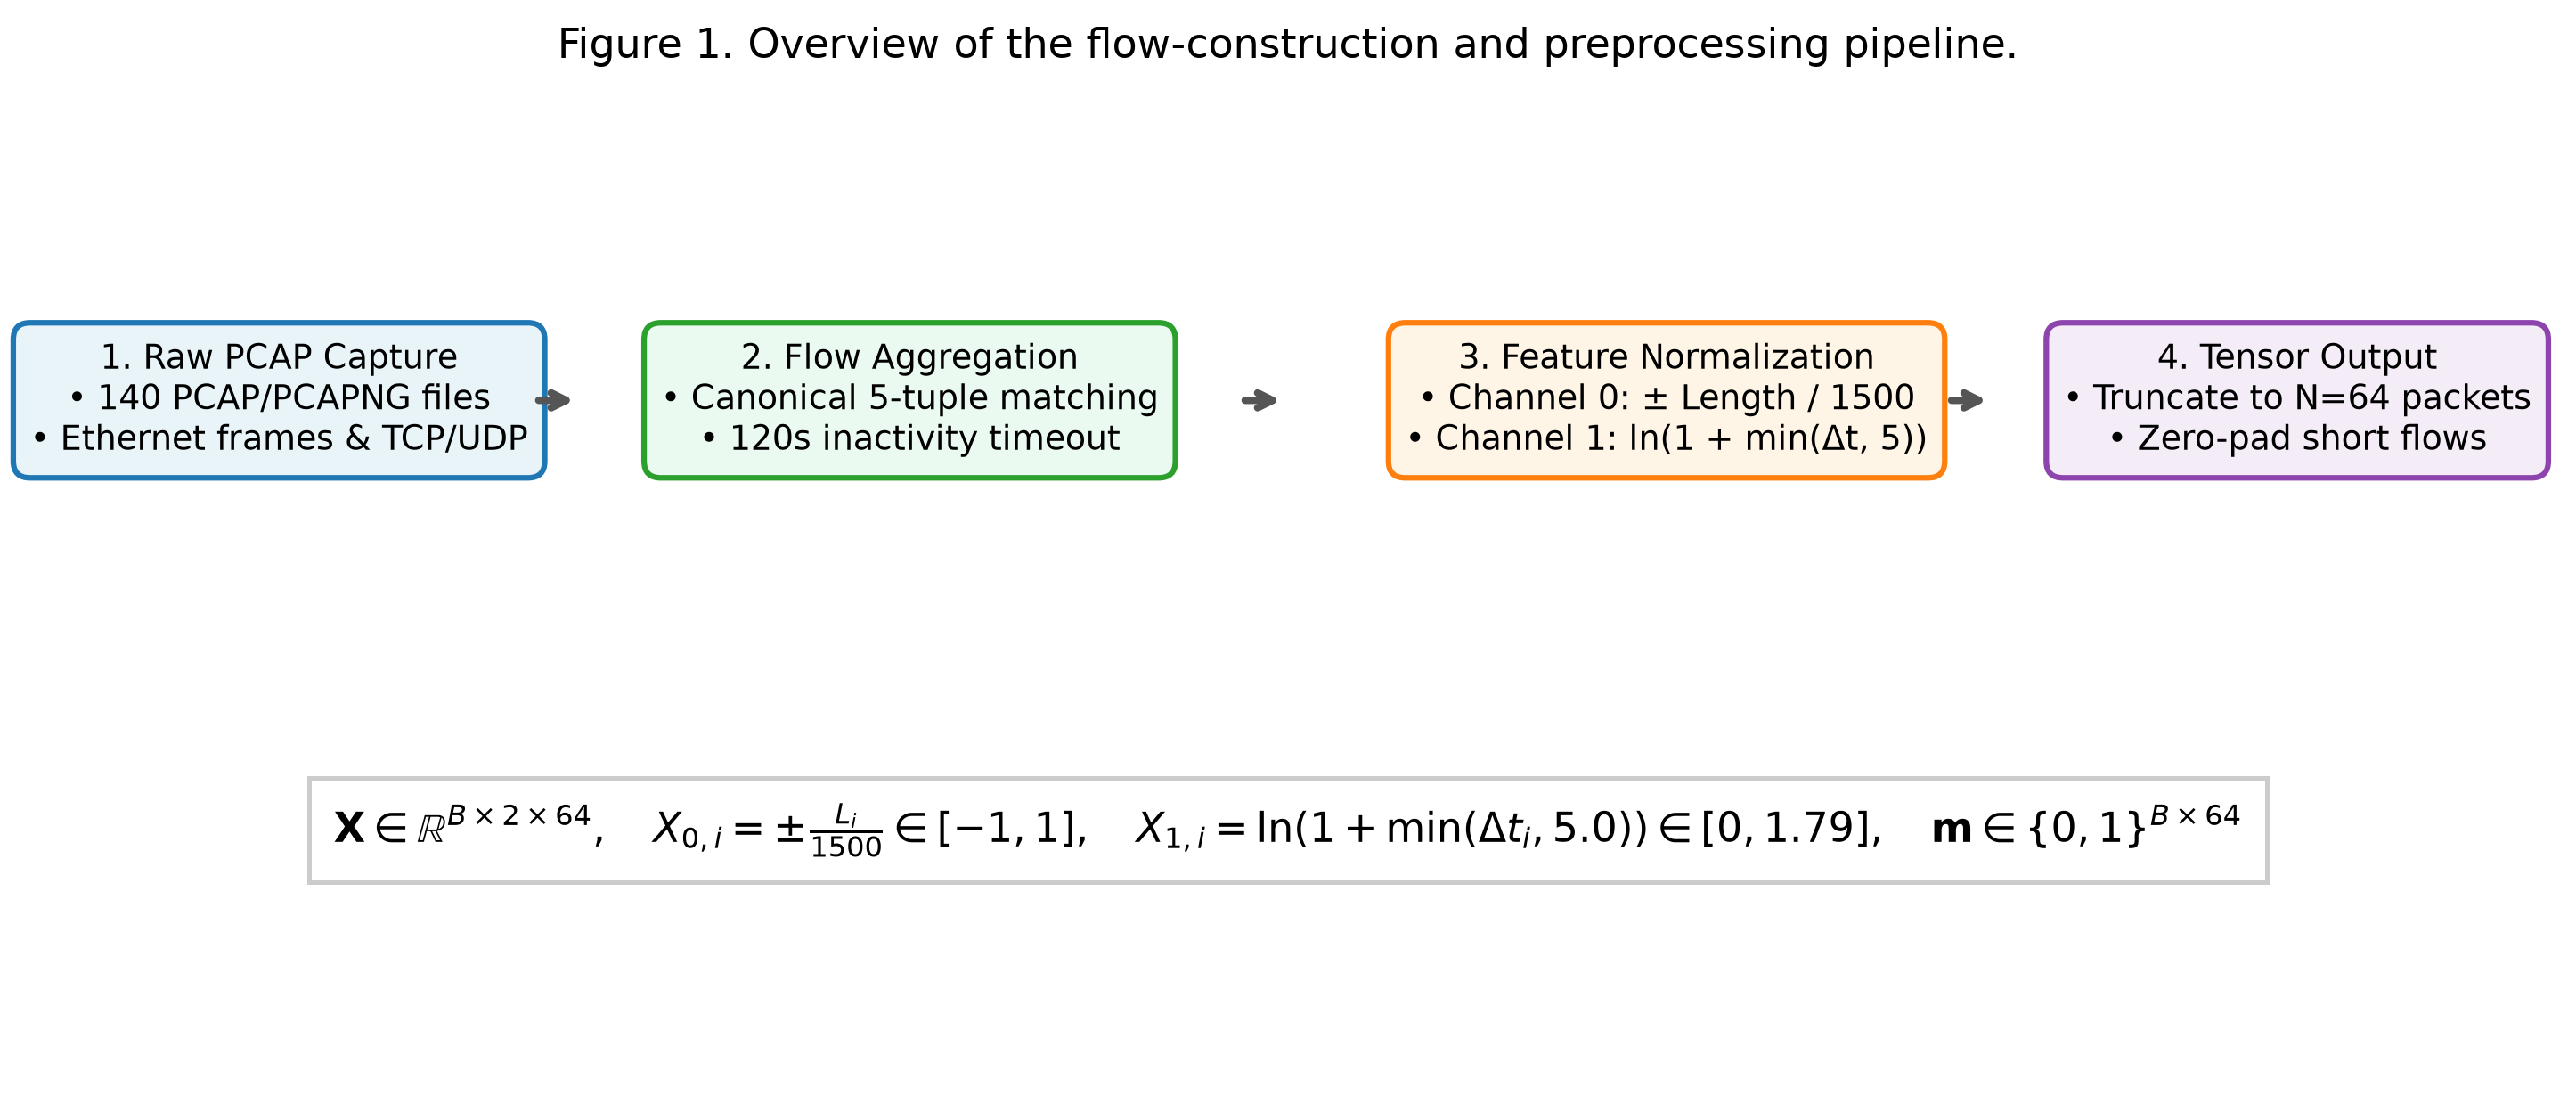
\includegraphics[width=\textwidth]{figures/figure1_flow_construction_pipeline.png}
\caption{End-to-end data ingestion, bidirectional flow canonicalization, and leakage-free canonical session partitioning architecture. Contrasts the flawed naive random split (cross-split leakage and session memorization) with the 106 canonical session group isolation protocol enforcing zero session contamination across train, validation, and test partitions.}
\label{fig:flow_ingestion_pipeline}
\end{figure*}

\subsection{Sequence Featurization and Observational Validity Masking}
\label{sec:featurization}
For each reassembled flow, we extract the temporal sequence of the first $L_{\max} = 64$ packets, constructing a standardized two-channel numerical tensor $\mathbf{X} \in \mathbb{R}^{2 \times 64}$. Selecting $L_{\max} = 64$ captures initial protocol handshake exchanges (TCP three-way handshake, TLS ClientHello/ServerHello, cipher suite negotiation, certificate exchange) while capping memory consumption at 512 bytes per flow:
\begin{enumerate}
    \item \textbf{Channel 0 (Directional Packet Length, $X_{0, t}$):} Represents the wire-level captured Ethernet frame length in bytes, signed by the transmission direction $d_t \in \{-1, +1\}$ and normalized by the standard Ethernet Maximum Transmission Unit (MTU = 1500 bytes):
    \begin{equation}
    X_{0, t} = d_t \cdot \min\left(1.0, \; \frac{\text{length}_t}{\text{MTU}}\right) \in [-1.0, \; +1.0]
    \label{eq:feat_len}
    \end{equation}
    \item \textbf{Channel 1 (Log-Scaled Inter-Arrival Time, $X_{1, t}$):} Encodes the elapsed interval $\Delta t_t = t_t - t_{t-1}$ between consecutive packet arrivals. Because raw inter-arrival times span six orders of magnitude (from microseconds to keep-alive pauses), intervals are clamped at $\Delta t_{\max} = 5.0\text{ s}$ and transformed via natural logarithm:
    \begin{equation}
    X_{1, t} = \frac{\ln(1 + \min(\Delta t_t, \; \Delta t_{\max}))}{\ln(1 + \Delta t_{\max})} \in [0.0, \; 1.0]
    \label{eq:feat_iat}
    \end{equation}
    For the initial packet ($t = 0$), inter-arrival time is defined relative to flow inception as $\Delta t_0 \equiv 0.0\text{ s}$, yielding $X_{1, 0} = 0.0$.
\end{enumerate}

\subsubsection{Active Sequence Masking}
Flows containing fewer than 64 packets (sequence length $L < 64$) are right-padded with zero values ($X_{0, t} = 0.0, X_{1, t} = 0.0$ for $t \ge L$). An observational validity mask $\mathbf{m} \in \{0, 1\}^{64}$ records active packet indices:
\begin{equation}
m_t = \begin{cases} 1, & 0 \le t < L \\ 0, & L \le t < 64 \end{cases}
\label{eq:mask}
\end{equation}
In our explainability audit, padded positions ($t \ge L$) are strictly masked out ($\phi_{0, t} \equiv 0, \phi_{1, t} \equiv 0$) to prevent artificial ranking similarity over synthetic zero tokens. Fig.~\ref{fig:featurization_schematic} illustrates this dual-channel sequence featurization and validity masking process.

\begin{figure}[t]
\centering
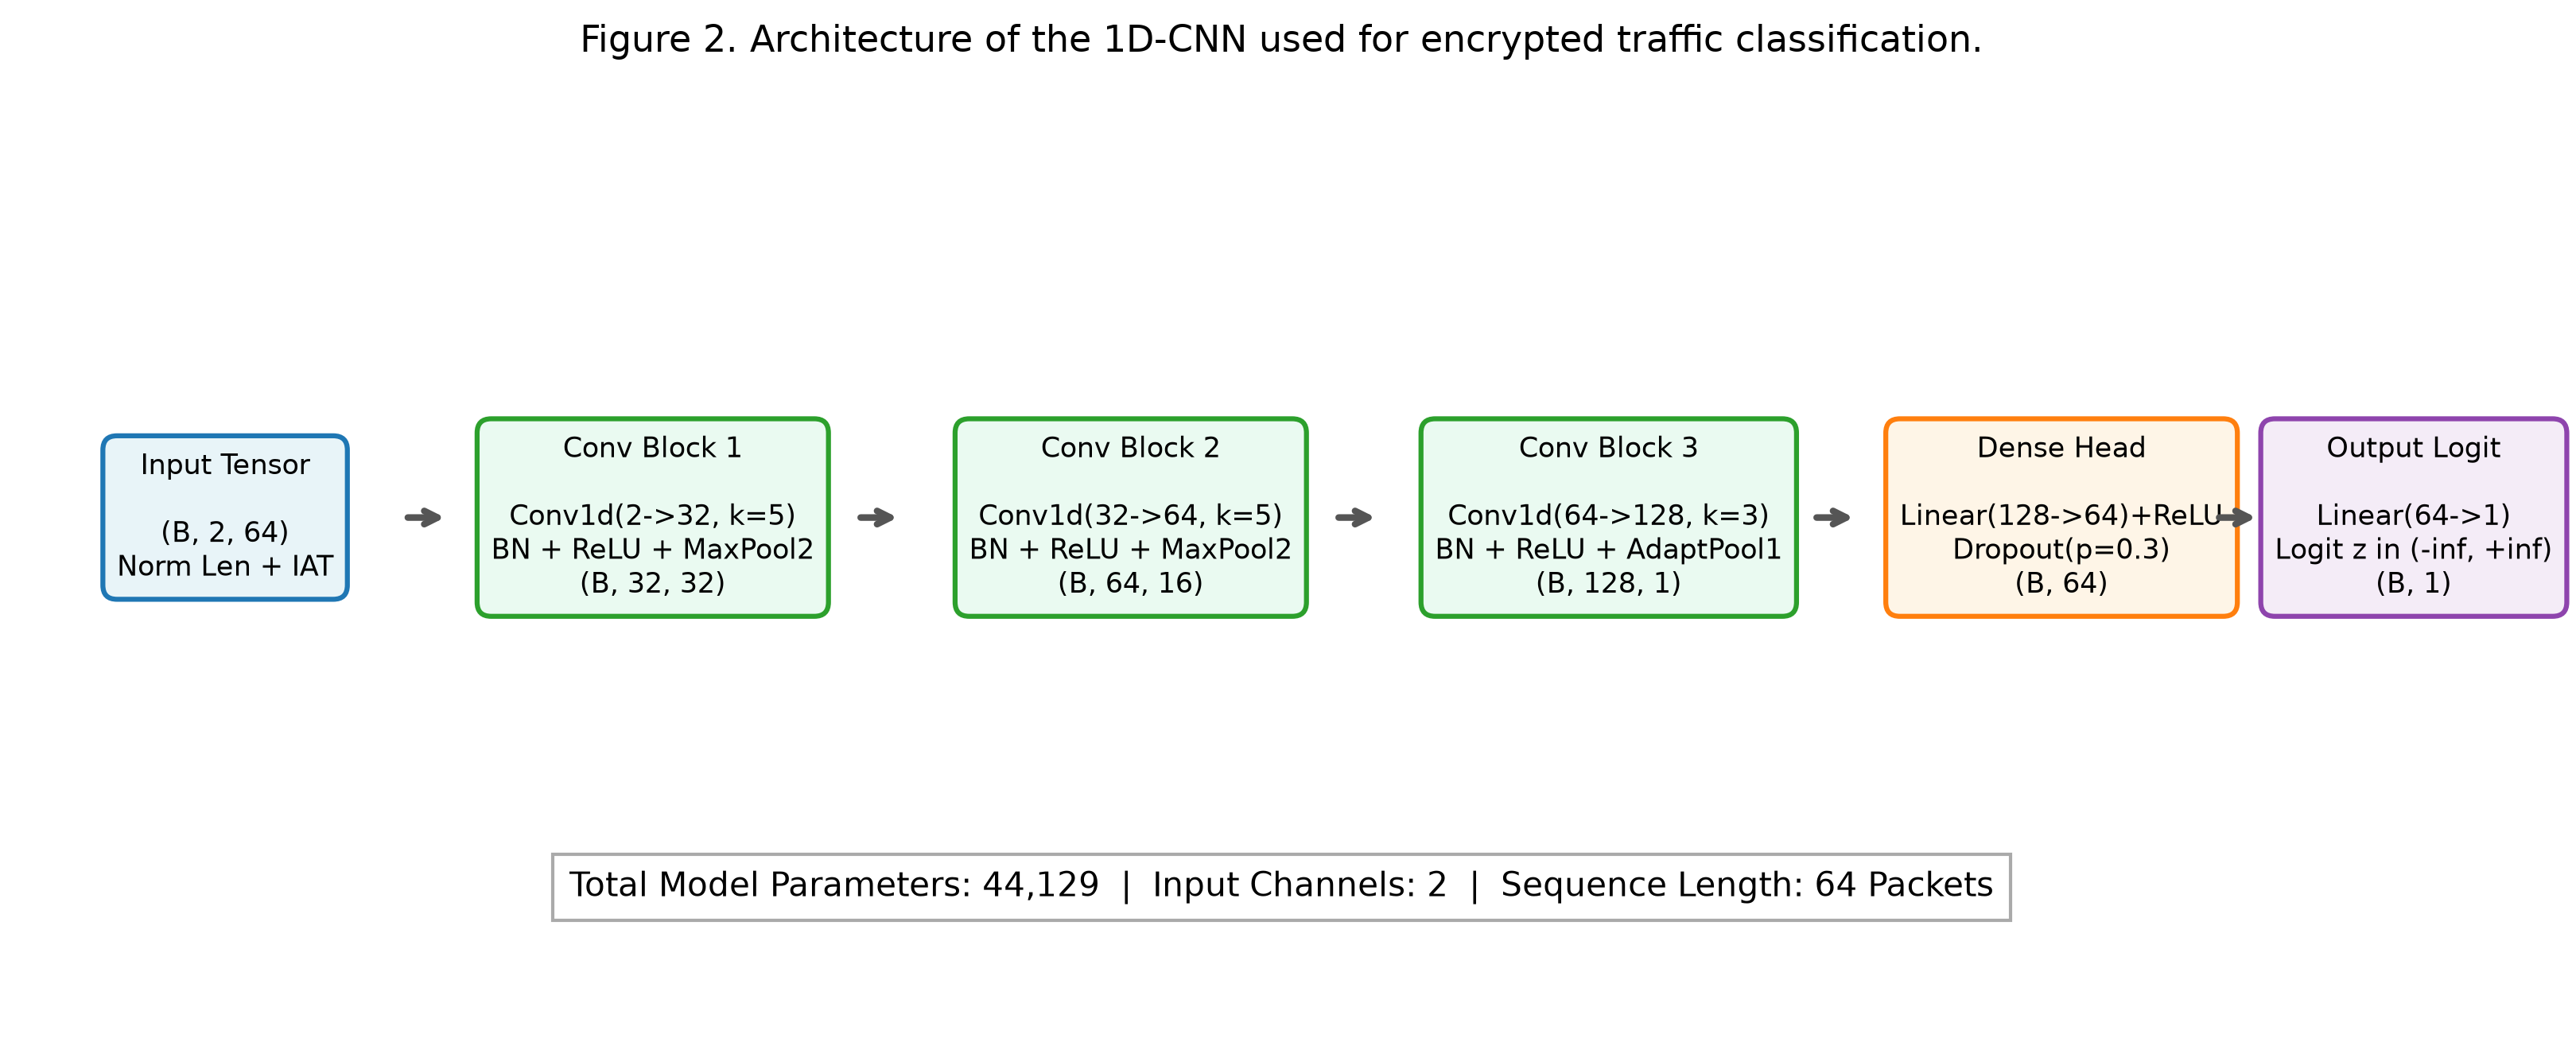
\includegraphics[width=\columnwidth]{figures/figure2_cnn1d_architecture.png}
\caption{Dual-channel temporal sequence featurization and observational validity masking. Raw packet sequences are mapped to signed directional lengths and log-scaled inter-arrival times, with active sequence masking invalidating padded tokens.}
\label{fig:featurization_schematic}
\end{figure}

\subsection{Deep Sequence Classifier: Traffic1DCNN Architecture}
\label{sec:architecture}
We formulate a lightweight 1D Convolutional Neural Network (\texttt{Traffic1DCNN}) engineered for line-rate execution within edge processor caches. The network comprises exactly \textbf{44,129 parameters} ($184.24\text{ KB}$ in full FP32 precision):
\begin{itemize}
    \item \textbf{Input Layer:} Ingests tensor $\mathbf{X} \in \mathbb{R}^{B \times 2 \times 64}$.
    \item \textbf{Block 1:} $\text{Conv1D}(2 \to 32, k=5, s=1, p=2) \to \text{BatchNorm1d}(32) \to \text{ReLU} \to \text{MaxPool1d}(2, s=2)$. Intermediate shape: $(B, 32, 32)$. Receptive field: $RF_1 = 6$ packets.
    \item \textbf{Block 2:} $\text{Conv1D}(32 \to 64, k=5, s=1, p=2) \to \text{BatchNorm1d}(64) \to \text{ReLU} \to \text{MaxPool1d}(2, s=2)$. Intermediate shape: $(B, 64, 16)$. Receptive field: $RF_2 = 14$ packets.
    \item \textbf{Block 3:} $\text{Conv1D}(64 \to 128, k=3, s=1, p=1) \to \text{BatchNorm1d}(128) \to \text{ReLU} \to \text{AdaptiveAvgPool1d}(1)$. Intermediate shape: $(B, 128, 1)$. Receptive field: $RF_3 = 24$ packets.
    \item \textbf{Classification Head:} $\text{Flatten} \to \text{Linear}(128 \to 64) \to \text{ReLU} \to \text{Dropout}(p=0.3) \to \text{Linear}(64 \to 1)$. Output: pre-sigmoid scalar logit $z \in \mathbb{R}$.
\end{itemize}
The global receptive field spans 24 consecutive packets, providing sufficient temporal context to capture early protocol handshake negotiations. The model is trained using AdamW ($lr = 10^{-3}$, $\beta_1 = 0.9, \beta_2 = 0.999$, weight decay $\lambda = 10^{-4}$, cosine annealing over 30 epochs, batch size 64). Checkpointing is performed at epoch 12 (\texttt{fp32\_seed\_42.pt}).

To address the $17.29:1$ class imbalance without synthetic oversampling, the Binary Cross-Entropy loss incorporates positive class weighting:
\begin{equation}
\mathcal{L}_{\text{BCE}} = -\frac{1}{N} \sum_{i=1}^N \left[ w_{\text{pos}} y_i \ln \sigma(z_i) + (1 - y_i) \ln(1 - \sigma(z_i)) \right]
\label{eq:bce_weighted}
\end{equation}
where $w_{\text{pos}} = 30.3756$ is derived analytically from the training partition class ratio ($N_{\text{neg}} / N_{\text{pos}}$).

\subsection{Fixed-Point Quantization Pipelines and Causal Control}
\label{sec:quantization}
Model quantization maps continuous 32-bit floating-point parameters to discrete 8-bit integers~\cite{b5},~\cite{b20}. Under uniform affine quantization, a real value $z \in \mathbb{R}$ is approximated by scale factor $s \in \mathbb{R}^+$ and zero-point offset $zp \in \mathbb{Z}$:
\begin{equation}
q = \text{clip}\left(\left\lfloor \frac{z}{s} \right\rceil + zp, \; q_{\min}, \; q_{\max}\right), \quad \tilde{z} = s \cdot (q - zp)
\label{eq:quant_affine}
\end{equation}
where $[q_{\min}, q_{\max}] = [-128, 127]$ for signed INT8 (\texttt{torch.qint8}) or $[0, 255]$ for unsigned INT8 (\texttt{torch.quint8}).

We evaluate three distinct compression and control branches:
\begin{enumerate}
    \item \textbf{Static Post-Training Quantization (PTQ):} The pre-trained FP32 model weights are quantized to symmetric signed 8-bit integers ($zp = 0, q \in [-128, 127]$) via \texttt{MinMaxObserver}. Activation scales and zero-points are calibrated by passing the 69,564 validation flows through the network using a \texttt{HistogramObserver} to record dynamic activation distributions without modifying model parameters. At deployment, PyTorch QNNPACK~\cite{b21} compiles the model into 8-bit integer kernels targeting ARM NEON vector instructions.
    \item \textbf{Quantization-Aware Training (QAT):} Forward activations and weights are quantized using simulated integer rounding operators, while the non-differentiable rounding step is bypassed during the backward pass using the Straight-Through Estimator (STE)~\cite{b22}:
    \begin{equation}
    \frac{\partial \tilde{z}}{\partial z} = \mathbf{1}_{|z - zp \cdot s| \le \frac{1}{2}(q_{\max} - q_{\min}) s}
    \label{eq:ste}
    \end{equation}
    The network is fine-tuned for 5 epochs with AdamW ($lr = 10^{-4}$, weight decay $10^{-5}$, batch size 64) to adapt weights to integer grid constraints.
    \item \textbf{The Unquantized Fine-Tuning Control (FP32-FT):} To establish whether attribution changes in QAT stem from integer quantization noise or from gradient-based parameter shifts across the empirical loss surface, we implement an unquantized control. FP32-FT undergoes the exact same 5-epoch AdamW schedule ($lr = 10^{-4}$, weight decay $10^{-5}$, $w_{\text{pos}} = 30.3756$) as QAT, but retains full 32-bit floating-point weights and activations without quantization operators.
\end{enumerate}

\subsubsection{The 2x2 Causal Factorial Disentanglement Formulation}
Let $\boldsymbol{\phi}(\mathcal{M})$ denote the feature attribution vector for model $\mathcal{M}$. The total attribution drift of QAT decomposes into orthogonal optimization and quantization vectors:
\begin{equation}
\Delta_{\text{total}}(\text{QAT}) = \underbrace{[\boldsymbol{\phi}(\text{FP32-FT}) - \boldsymbol{\phi}(\text{FP32})]}_{\text{Optimization Drift } \Delta_{\text{opt}}} + \underbrace{[\boldsymbol{\phi}(\text{QAT}) - \boldsymbol{\phi}(\text{FP32-FT})]}_{\text{Quantization Noise } \Delta_{\text{quant}}}
\label{eq:causal_decomp}
\end{equation}
By comparing QAT directly against FP32-FT, we isolate $\Delta_{\text{quant}}$ from optimization artifacts. Fig.~\ref{fig:quantization_workflows} illustrates this $2 \times 2$ causal disentanglement matrix and the corresponding quantization workflows.

\begin{figure*}[t]
\centering
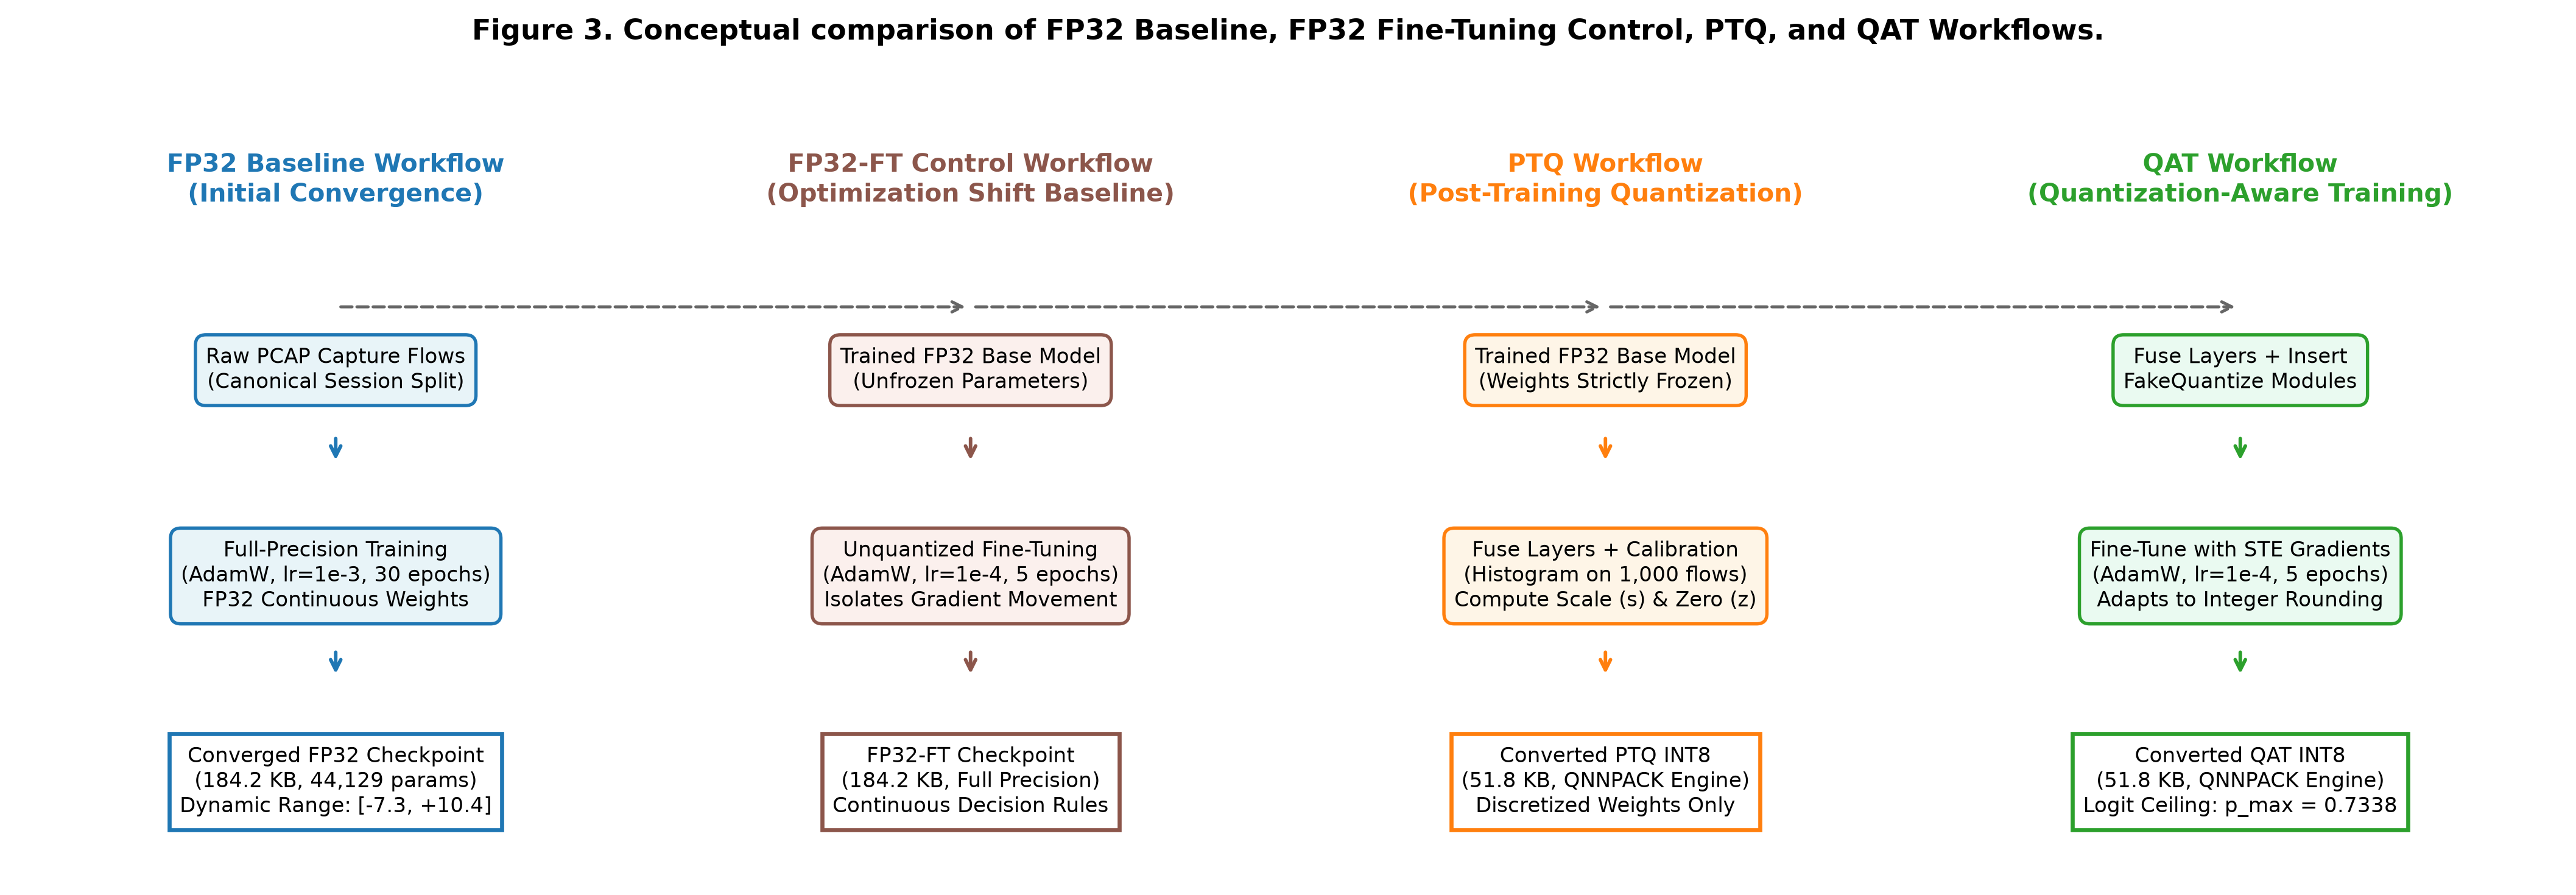
\includegraphics[width=\textwidth]{figures/figure3_quantization_workflows.png}
\caption{The $2 \times 2$ causal factorial disentanglement matrix and tri-branch quantization workflows. Factorial matrix isolates continuous optimization drift ($\Delta_{\text{opt}}$) from discrete fixed-point quantization noise ($\Delta_{\text{quant}}$) by pairing INT8-QAT with an unquantized fine-tuning control (FP32-FT).}
\label{fig:quantization_workflows}
\end{figure*}

\subsubsection{Mechanistic Proof of Output Saturation}
In serialized QAT execution under PyTorch QNNPACK, the output dequantization node transforms the quantized integer output $q_{\text{out}}$ to continuous logit $z$ via affine mapping:
\begin{equation}
z = s_{\text{out}} \cdot (q_{\text{out}} - zp_{\text{out}})
\label{eq:dequant_out}
\end{equation}
where calibration yields scale $s_{\text{out}} = 0.02535125$ and zero-point offset $zp_{\text{out}} = 215$. Because $q_{\text{out}}$ is bounded by the unsigned 8-bit integer maximum $q_{\max} = 255$, the reachable pre-sigmoid logit is strictly capped:
\begin{equation}
z_{\max} = s_{\text{out}} \cdot (q_{\max} - zp_{\text{out}}) = 0.02535125 \times (255 - 215) = +1.014050
\label{eq:z_max}
\end{equation}
This logit ceiling establishes an absolute upper bound on the sigmoid classification probability:
\begin{equation}
p_{\max} = \sigma(+1.014050) = \frac{1}{1 + e^{-1.014050}} = 0.733812
\label{eq:p_max}
\end{equation}
Applying the default uncalibrated FP32 threshold ($\tau = 0.900$) to QAT guarantees that $p_i < \tau$ for all flows, causing 100\% false negatives (recall = 0.0\%, F1 = 0.0000). To restore operational validity, we perform post-quantization validation calibration on the 69,564 validation flows, selecting $\tau_{\text{cal}} = 0.680$ to recover classification F1 to $77.62\%$.

\subsection{Model-Agnostic Explainability Audit via Masked KernelSHAP}
\label{sec:kernel_shap}
Evaluating feature attribution stability on deployed edge hardware requires an explainer compatible with discrete integer execution. Backpropagation-based attribution methods (such as Integrated Gradients~\cite{b23} or DeepLIFT) require continuous gradient access $\nabla_{\mathbf{X}} f(\mathbf{X})$. On physical edge hardware running compiled INT8 assembly (e.g., PyTorch QNNPACK), computational graphs contain step functions whose analytical gradients are zero almost everywhere:
\begin{equation}
\frac{\partial}{\partial z} \lfloor z \rceil = 0 \quad \text{a.e.}
\label{eq:zero_grad}
\end{equation}
Because compiled integer graphs evaluate to zero gradients almost everywhere, analytical gradient explainers cannot execute on deployed runtimes.

We employ \textbf{KernelSHAP}~\cite{b4}, a perturbation-based, model-agnostic attribution framework rooted in cooperative game theory. KernelSHAP treats the model as an opaque black-box oracle $f: \mathbb{R}^D \to \mathbb{R}$, querying pre-sigmoid classification logits $z = f(\mathbf{x})$ across $D = 128$ flattened sequence features:
\begin{equation}
f(\mathbf{x}) = \phi_0 + \sum_{j=1}^{128} \phi_j(\mathbf{x})
\label{eq:shap_efficiency}
\end{equation}
where $\phi_0 = \mathbb{E}_{\mathbf{x}' \sim \mathcal{D}_{\text{bg}}}[f(\mathbf{x}')]$ represents the baseline expected logit over background reference set $\mathcal{D}_{\text{bg}}$. Missing features in coalition subsets are integrated out against $M = 50$ randomly sampled Non-VPN training flows. Each flow evaluation evaluates $K = 150$ coalition samples, solving the weighted linear regression under the Shapley kernel:
\begin{equation}
\pi_{\mathbf{x}}(z') = \frac{D - 1}{\binom{D}{|z'|} |z'| (D - |z'|)}
\label{eq:shap_kernel}
\end{equation}
Axiomatic efficiency was verified across all evaluated flows: the maximum additivity residual $|\sum_j \phi_j - (f(\mathbf{x}) - \phi_0)|$ was strictly bounded below $7.15 \times 10^{-6}$.

\subsubsection{Stratified Test Cohort and Padding Masking}
Auditing KernelSHAP across all 49,251 test flows requires over $369\text{ million}$ forward passes, which is computationally intractable for edge audit routines ($> 400\text{ CPU hours}$). We therefore draw a stratified cohort of $N = 100$ test flows:
\begin{itemize}
    \item Exactly 50 VPN flows and 50 Non-VPN flows, balancing class representation.
    \item Flows drawn uniformly across all 16 completely held-out canonical test sessions.
    \item Sequence lengths stratified uniformly from short bursts ($L = 4$) to full sequences ($L = 64$).
\end{itemize}
To ensure methodological validity, we enforce \textbf{observational sequence masking}: for any flow with $L < 64$, Shapley attributions for padded positions ($t \ge L$) are explicitly set to zero ($\phi_{0, t} \equiv 0, \phi_{1, t} \equiv 0$). Attribution metrics are evaluated exclusively over active packet tokens.

\subsection{Quantitative Attribution Drift Metrics and Explainer Noise Floor}
\label{sec:drift_metrics}
Attribution drift is measured across four complementary mathematical dimensions between a baseline attribution vector $\mathbf{a}^{\text{ref}} \in \mathbb{R}^D$ and a target attribution vector $\mathbf{a}^{\text{tgt}} \in \mathbb{R}^D$:
\begin{enumerate}
    \item \textbf{Top-$k$ Intersection-over-Union ($\text{IoU}_k$):} The Jaccard similarity between the sets of $k$ largest attribution magnitudes, evaluated at $k = 5$ and $k = 10$:
    \begin{equation}
    \text{IoU}_k(\mathbf{a}^{\text{ref}}, \mathbf{a}^{\text{tgt}}) = \frac{|\mathcal{T}_k(\mathbf{a}^{\text{ref}}) \cap \mathcal{T}_k(\mathbf{a}^{\text{tgt}})|}{|\mathcal{T}_k(\mathbf{a}^{\text{ref}}) \cup \mathcal{T}_k(\mathbf{a}^{\text{tgt}})|}
    \label{eq:iou_k}
    \end{equation}
    where $\mathcal{T}_k(\mathbf{a})$ denotes the set of feature indices corresponding to the $k$ largest absolute attribution values.
    \item \textbf{Total Variation Distance ($TV$):} The normalized attribution mass displacement:
    \begin{equation}
    TV(\mathbf{a}^{\text{ref}}, \mathbf{a}^{\text{tgt}}) = \frac{1}{2} \sum_{i=1}^D \left| \frac{a_i^{\text{ref}}}{\sum_m |a_m^{\text{ref}}|} - \frac{a_i^{\text{tgt}}}{\sum_m |a_m^{\text{tgt}}|} \right| \in [0.0, \; 1.0]
    \label{eq:tv}
    \end{equation}
    \item \textbf{Signed Cosine Similarity ($S_c$):} The directional orientation between attribution vectors in $D$-dimensional space:
    \begin{equation}
    S_c(\mathbf{a}^{\text{ref}}, \mathbf{a}^{\text{tgt}}) = \frac{\mathbf{a}^{\text{ref}} \cdot \mathbf{a}^{\text{tgt}}}{\|\mathbf{a}^{\text{ref}}\|_2 \|\mathbf{a}^{\text{tgt}}\|_2} \in [-1.0, \; +1.0]
    \label{eq:cosine}
    \end{equation}
    \item \textbf{Spearman Rank Correlation ($r_s$):} The monotonic ranking consistency across active feature positions:
    \begin{equation}
    r_s = 1 - \frac{6 \sum_{i=1}^D d_i^2}{D(D^2 - 1)}
    \label{eq:spearman}
    \end{equation}
    where $d_i = \text{rank}(a_i^{\text{ref}}) - \text{rank}(a_i^{\text{tgt}})$.
\end{enumerate}

\subsubsection{The Multi-Seed Explainer Noise Floor}
Perturbation explainers contain inherent Monte Carlo sampling variance. To separate true model attribution drift from explainer stochasticity, we establish an empirical \textbf{Explainer Noise Floor}. We execute KernelSHAP across three independent random seeds (Seeds 42, 43, 44) on the identical, uncompressed FP32 model. The pairwise differences across seeds define the baseline repeatability boundary ($\text{IoU}_5 = 0.9553 \pm 0.1829$, $TV = 0.0553 \pm 0.1588$, $S_c = 0.9676 \pm 0.1450$). Any cross-model drift failing to exceed these boundaries cannot be distinguished from explainer sampling jitter. Fig.~\ref{fig:kernel_shap_noise_floor} illustrates the complete KernelSHAP audit protocol, zero-padding masking, and the multi-seed explainer noise floor repeatability boundary.

\begin{figure*}[t]
\centering
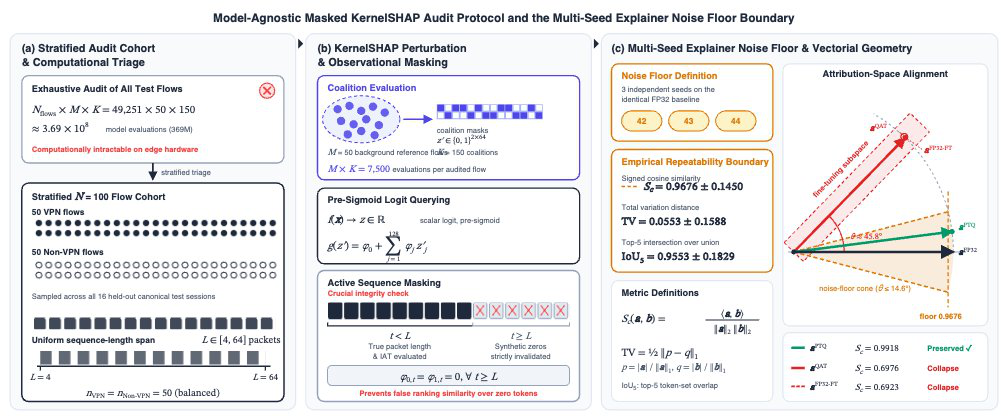
\includegraphics[width=\textwidth]{figures/figure6_kernel_shap_noise_floor.png}
\caption{Model-Agnostic Masked KernelSHAP Audit Protocol and the Multi-Seed Explainer Noise Floor Boundary. (a) Stratified computational triage reducing 369M evaluations to a representative $N=100$ cohort (50 VPN, 50 Non-VPN). (b) Black-box coalition evaluation over $M=50$ background reference flows with active sequence masking strictly invalidating padded tokens ($\phi_{0,t} \equiv 0, \phi_{1,t} \equiv 0, \forall t \ge L$). (c) Empirical multi-seed repeatability boundary (Seeds 42, 43, 44; $S_c = 0.9676 \pm 0.1450, TV = 0.0553 \pm 0.1588, \text{IoU}_5 = 0.9553 \pm 0.1829$) and attribution-space alignment demonstrating that INT8-PTQ preserves explanation geometry within the noise-floor cone ($\theta \le 14.6^\circ, S_c = 0.9918$), while INT8-QAT ($S_c = 0.4830$ overall, collapsing to $S_c = 0.1665$ on VPN flows) departs markedly from the noise-floor boundary.}
\label{fig:kernel_shap_noise_floor}
\end{figure*}

\subsection{Clustered Statistical Inference Formulation}
\label{sec:clustered_inference}
Network flows collected during a single capture session share operating system network stacks, congestion control state, and environmental background noise, violating the independent and identically distributed (IID) assumption~\cite{b24}. Evaluating flow-level predictions with standard unclustered statistical tests produces severe standard error deflation (up to $56\times$), yielding spurious rejection of the null hypothesis and artificially narrow confidence intervals.

To model session-level clustering, we formulate two distinct statistical estimands across the $K = 16$ canonical test sessions:
\begin{enumerate}
    \item \textbf{Estimand A (Flow-Weighted Pooled Mean):} The aggregate mean logit shift weighted by session flow volume $n_k$:
    \begin{equation}
    \Delta \bar{z}_{\text{flow}} = \frac{1}{\sum_{k=1}^K n_k} \sum_{k=1}^K \sum_{i=1}^{n_k} (z_{k, i}^{\text{PTQ}} - z_{k, i}^{\text{FP32}}) = -0.0778
    \label{eq:estimand_a}
    \end{equation}
    with 95\% cluster bootstrap confidence interval $[-0.1124, +0.3275]$ (spans zero).
    \item \textbf{Estimand B (Session-Macro Unweighted Mean):} The unweighted arithmetic average of session-level mean shifts:
    \begin{equation}
\Delta \bar{z}_{\text{session}} = \frac{1}{K} \sum_{k=1}^K \overline{\Delta z}_k = \frac{1}{K} \sum_{k=1}^K \left( \frac{1}{n_k} \sum_{i=1}^{n_k} (z_{k, i}^{\text{PTQ}} - z_{k, i}^{\text{FP32}}) \right) = +0.2270
\label{eq:estimand_b}
\end{equation}
    with 95\% cluster bootstrap confidence interval $[+0.0630, +0.3554]$ (strictly positive).
\end{enumerate}
Estimand A evaluates the specific test pool, which is heavily dominated by a single massive capture session (\texttt{skype\_audio3}, containing 39,179 flows or $79.55\%$ of the test set). Estimand B evaluates expected generalization to new, unobserved network recording sessions, where 13 out of 16 sessions exhibit positive logit shifts. We evaluate inferential uncertainty using a 	extbf{16-group cluster bootstrap resampling protocol} ($B = 2,000$ resamples of whole canonical sessions with replacement), producing cluster-consistent confidence intervals that account for intra-session correlation.

\section{Experimental Results}

In this section, we evaluate the computational efficiency, predictive classification performance, probability calibration dynamics, explainability fidelity, and clustered statistical stability of 32-bit floating-point (FP32), an unquantized Fine-Tuned control baseline (FP32-FT), static Post-Training Quantized (INT8-PTQ), and Quantization-Aware Trained (INT8-QAT) models under the PyTorch QNNPACK execution engine. Predictive classification and probability calibration dynamics are evaluated across the full held-out test partition ($N = 49,251$ bidirectional flows across 16 canonical capture groups), ensuring zero cross-split session contamination. Owing to the computational cost of perturbation-based Shapley sampling (50 background reference flows $\times$ 150 coalition evaluations per flow), feature attribution drift is rigorously evaluated on a representative, stratified cohort of $N = 100$ test flows (50 VPN and 50 Non-VPN flows).

\subsection{Computational Efficiency and Hardware Benchmarking}

We evaluate physical execution metrics on edge hardware to determine whether 8-bit integer quantization delivers concrete latency and throughput benefits for network traffic inspection. Profiling was conducted on an Apple Silicon ARM64 processor (macOS 15.1) using the PyTorch QNNPACK execution engine. All benchmarks reflect 500 timed evaluation passes following 50 warm-up runs. Table~\ref{tab:hardware} summarizes the measured checkpoint footprints, per-flow latencies, and throughput rates across streaming and batched operational modes.

\begin{table}[htbp]
\caption{Hardware Performance and Edge Storage Benchmarks}
\label{tab:hardware}
\centering
\footnotesize
\setlength{\tabcolsep}{3pt}
\begin{tabular}{lccc}
\toprule
\textbf{Metric} & \textbf{FP32} & \textbf{INT8-PTQ} & \textbf{INT8-QAT} \\
\midrule
Checkpoint Size & 184.24 KB & 51.77 KB & 51.77 KB \\
Compression Ratio & $1.00\times$ & $\mathbf{3.56\times}$ & $\mathbf{3.56\times}$ \\
L1-D Fit ($\le 64\,$KB) & Exceeds & Fits & Fits \\
\midrule
\multicolumn{4}{l}{\textit{Streaming Inspection ($B = 1$)}} \\
Median Latency & 0.267 ms & 0.255 ms & 0.242 ms \\
Latency Speedup & $1.00\times$ & $1.05\times$ & $1.10\times$ \\
Throughput (flows/s) & 3,439 & \textbf{3,797} & \textbf{4,005} \\
Throughput Speedup & $1.00\times$ & $\mathbf{1.10\times}$ & $\mathbf{1.16\times}$ \\
\midrule
\multicolumn{4}{l}{\textit{Micro-Batched ($B = 64$)}} \\
Median Latency & 9.503 ms & 0.764 ms & 0.755 ms \\
Latency Speedup & $1.00\times$ & $\mathbf{12.44\times}$ & $\mathbf{12.59\times}$ \\
Throughput (flows/s) & 6,387 & 76,265 & 81,552 \\
Throughput Speedup & $1.00\times$ & $\mathbf{11.94\times}$ & $\mathbf{12.77\times}$ \\
\bottomrule
\end{tabular}
\end{table}

\begin{figure}[htbp]
\centering
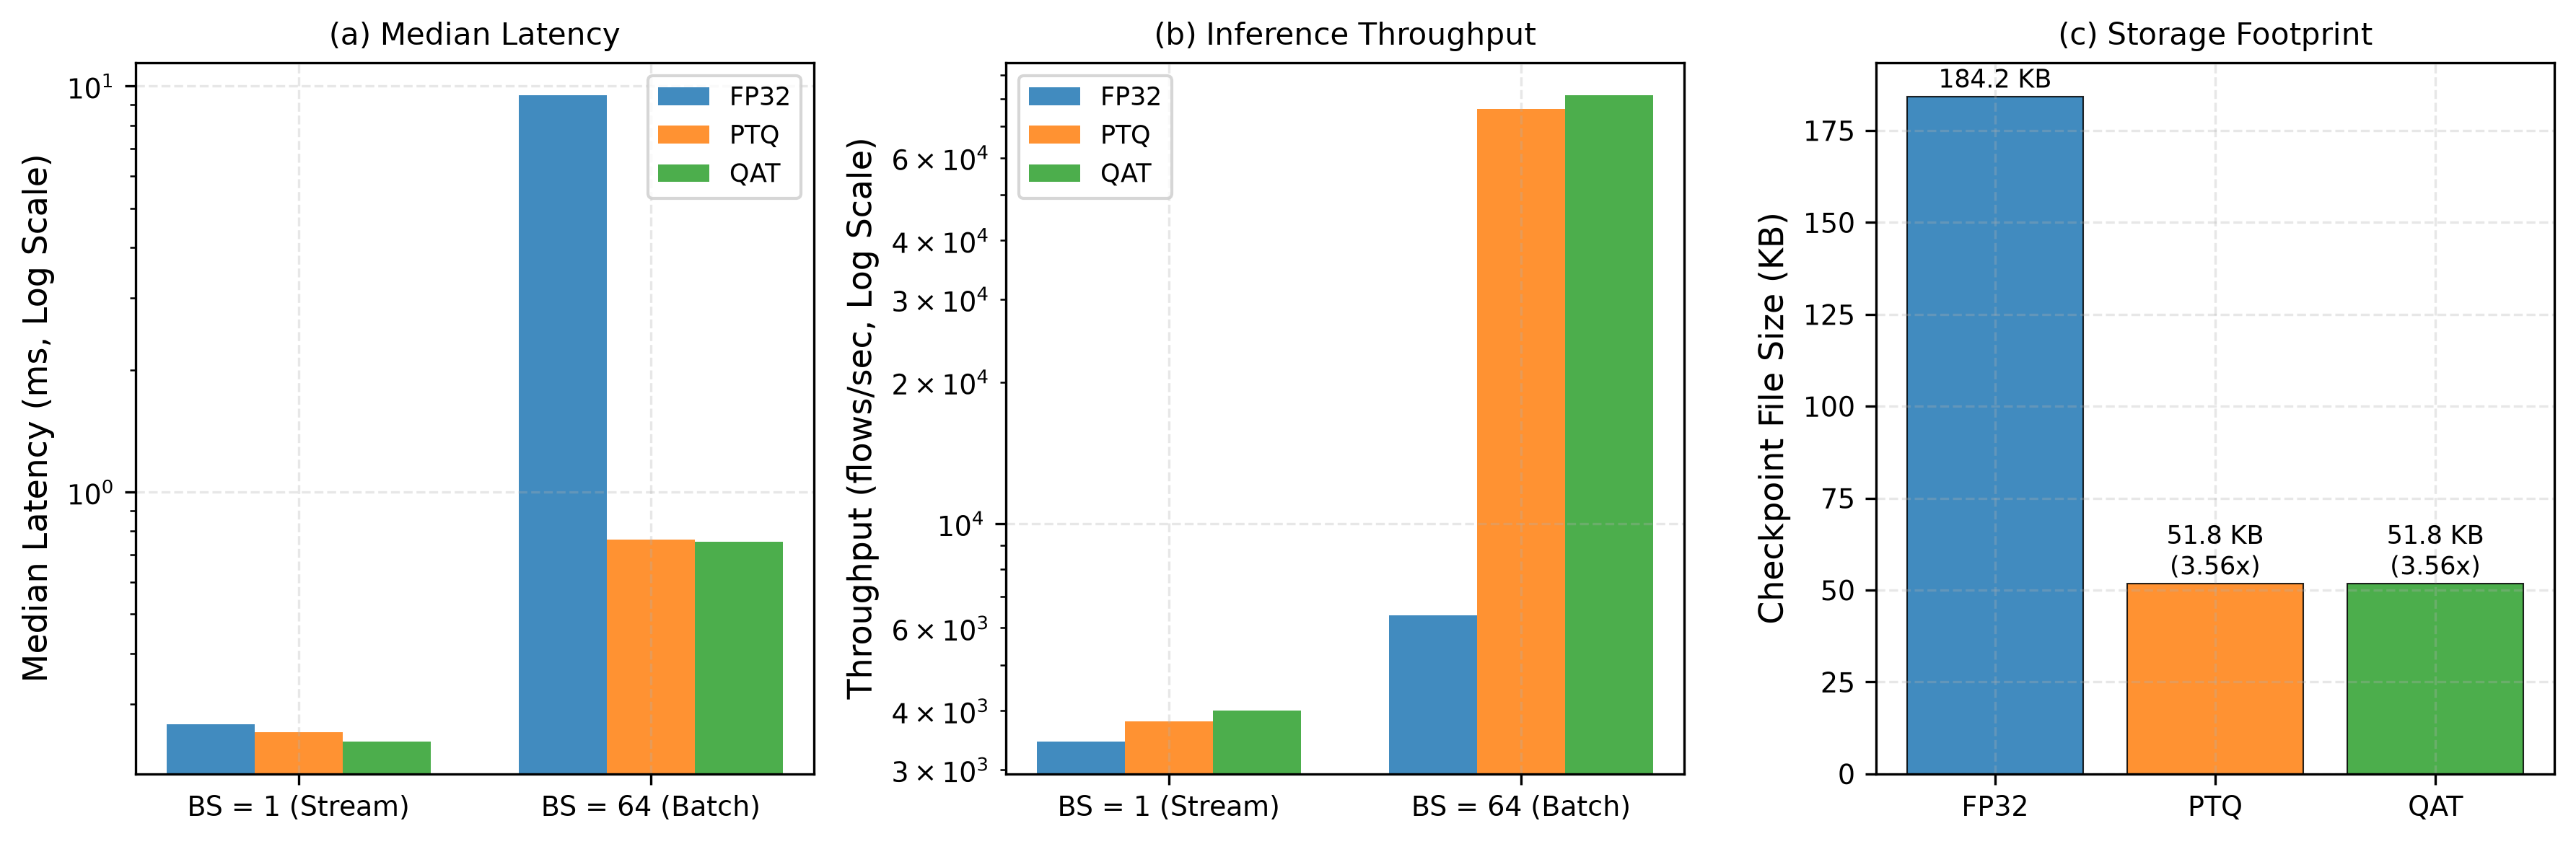
\includegraphics[width=\columnwidth]{figures/figure17_inference_latency.png}
\caption{Inference latency across precision formats under single-flow streaming ($B=1$) and micro-batched ($B=64$) execution on ARM64 hardware (500 timed runs, log scale).}
\label{fig:latency}
\end{figure}

Quantization compresses the serialized model checkpoint from 184.24 KB to 51.77 KB, yielding a $3.56\times$ storage reduction. This reduction provides direct microarchitectural benefits for edge deployments. Typical embedded ARM cores (e.g., ARM Cortex-A efficiency cores) provide a 64 KB per-core L1 data cache allocation. At 184.24 KB, the uncompressed FP32 parameters exceed this threshold by nearly $3\times$, guaranteeing that filter weights cannot remain resident across layer evaluations without triggering cache evictions to slower L2 cache or system DRAM. In contrast, the 51.77 KB INT8 static parameter footprint fits comfortably within a 64 KB L1-D cache budget, enabling persistent weight residency across successive inference cycles. Although the total runtime working set at larger batch sizes also encompasses dynamic intermediate activations and scratchpad buffers that spill into L2 cache, keeping static weights compact substantially alleviates memory bus contention.

The timing measurements reveal an operational division between streaming packet inspection and batched traffic triage:

\textbf{Streaming Inspection ($B = 1$):} When classifying isolated flows one by one, integer quantization yields modest latency gains. Median per-flow latency decreases from 0.267 ms in FP32 to 0.255 ms in PTQ ($1.05\times$ latency speedup) and 0.242 ms in QAT ($1.10\times$ latency speedup). Processing throughput increases modestly from 3,439 flows/s in FP32 to 3,797 flows/s in PTQ ($1.10\times$ throughput speedup) and 4,005 flows/s in QAT ($1.16\times$ throughput speedup). 

This modest gain stems from framework execution limits. The 1D-CNN contains 44,129 parameters, requiring approximately $8.8 \times 10^4$ multiply-accumulate operations per flow. On an ARM processor operating at gigahertz clock rates, the theoretical compute time for these operations is under one microsecond. Yet the measured execution time is roughly 250 microseconds. Over 99\% of wall-clock time at batch size 1 is absorbed by Python runtime interpretation, tensor memory allocations, operator dispatch, and quantization scale conversions. Because arithmetic execution accounts for less than 1\% of latency, replacing floating-point operations with integer math produces negligible savings in streaming mode.

\textbf{Micro-Batched Triage ($B = 64$):} When traffic can be accumulated into small buffers of 64 flows, framework invocation costs are amortized across the batch, shifting execution into a compute-bound state. In this regime, INT8 quantization accelerates processing substantially. Median batch latency drops from 9.503 ms down to 0.764 ms under PTQ ($12.44\times$ speedup) and 0.755 ms under QAT ($12.59\times$ speedup). As shown in Fig.~\ref{fig:latency}, this translates to an order-of-magnitude reduction in execution delay. Batched throughput scales from 6,387 flows/s in FP32 to 76,265 flows/s in PTQ ($11.94\times$ gain) and 81,552 flows/s in QAT ($12.77\times$ gain).

This 12-fold acceleration is driven by ARM NEON SIMD vectorization. ARM64 processors feature 128-bit vector registers. While a single 128-bit register holds four 32-bit floats, it packs sixteen 8-bit integers. With specialized dot-product instructions, the hardware processes four 8-bit integer multiply-accumulates into 32-bit accumulators in a single instruction cycle. In addition, INT8 reduces memory bus traffic by 75\%, loading 64 weights per standard 64-byte cache line instead of 16. In streaming per-packet deployments, software overhead dominates; in batched traffic collectors, integer SIMD execution delivers the throughput necessary to inspect high-rate network backbones.

\subsection{Predictive Performance and Decision Threshold Dynamics}

We evaluate predictive classification performance on the full held-out test partition, comprising $N = 49,251$ bidirectional flows (2,693 true VPN flows and 46,558 true Non-VPN flows). This split reflects the operational class imbalance common in production networks, where tunneling traffic constitutes a 5.47\% minority. All test flows originate from 16 canonical capture sessions that share zero session overlap with training or validation splits. Table~\ref{tab:predictive} reports discrimination metrics across three operational perspectives: threshold-independent ranking (Panel A), validation-calibrated operating points (Panel B), and an uncalibrated scenario where the baseline threshold is transferred directly to quantized models (Panel C).

\begin{table*}[htbp]
\caption{Predictive Performance on Held-Out Test Set ($N=49,251$)}
\label{tab:predictive}
\centering
\begin{tabular}{lcccccc}
\toprule
\textbf{Metric} & \textbf{FP32 Baseline} & \textbf{FP32-FT (Control)} & \textbf{INT8-PTQ} & \textbf{$\Delta$ (PTQ)} & \textbf{INT8-QAT} & \textbf{$\Delta$ (QAT)} \\
\midrule
\multicolumn{7}{l}{\textbf{Panel A: Threshold-Independent Ranking Performance}} \\
ROC-AUC & 0.9796 & 0.9819 & 0.9785 & $-0.0012$ & \textbf{0.9834} & $+0.0038$ \\
PR-AUC (Minority VPN) & 0.5610 & 0.6128 & 0.6102 & $+0.0492$ & \textbf{0.6478} & $+0.0868$ \\
Brier Score & 0.0585 & 0.0248 & 0.0584 & $-0.0000$ & \textbf{0.0237} & $-0.0347$ \\
\midrule
\multicolumn{7}{l}{\textbf{Panel B: Model-Specific Validation-Calibrated Operating Points}} \\
Decision Threshold ($\tau$) & 0.900 & 0.830 & 0.900 & $+0.000$ & 0.680 & $-0.220$ \\
Accuracy & 96.88\% & \textbf{97.64\%} & 96.79\% & $-0.09\%$ & 96.90\% & $+0.02\%$ \\
Balanced Accuracy & 97.41\% & 97.25\% & 97.41\% & $+0.00\%$ & \textbf{97.57\%} & $+0.17\%$ \\
Precision (VPN) & 64.04\% & \textbf{70.77\%} & 63.33\% & $-0.71\%$ & 64.12\% & $+0.08\%$ \\
Recall (VPN) & 97.99\% & 96.81\% & 98.11\% & $+0.11\%$ & \textbf{98.33\%} & $+0.33\%$ \\
$F_1$-Score & 0.7746 & \textbf{0.8176} & 0.7697 & $-0.0049$ & 0.7762 & $+0.0016$ \\
Positive Calls (Predicted VPN) & 4,121 & 3,684 & 4,172 & $+51$ & 4,130 & $+9$ \\
True Positives / False Negatives & 2,639 / 54 & 2,607 / 86 & 2,642 / 51 & $+3 / -3$ & \textbf{2,648 / 45} & $+9 / -9$ \\
\midrule
\multicolumn{7}{l}{\textbf{Panel C: Reused Baseline Threshold ($\tau = 0.900$, Uncalibrated Comparison)}} \\
Positive Calls (Predicted VPN) & 4,121 & 1,693 & 4,172 & $+51$ & \textbf{0} & $-4,121$ \\
Accuracy & 96.88\% & 94.45\% & 96.79\% & $-0.09\%$ & 94.53\% & $-2.35\%$ \\
Balanced Accuracy & 97.41\% & 64.42\% & 97.41\% & $+0.00\%$ & \textbf{50.00\%} & $-47.41\%$ \\
Precision (VPN) & 64.04\% & 48.85\% & 63.33\% & $-0.71\%$ & \textbf{0.00\%} & $-64.04\%$ \\
Recall (VPN) & 97.99\% & 30.71\% & 98.11\% & $+0.11\%$ & \textbf{0.00\%} & $-97.99\%$ \\
$F_1$-Score & 0.7746 & 0.3771 & 0.7697 & $-0.0049$ & \textbf{0.0000} & $\mathbf{-0.7746}$ \\
Missed VPN Flows (False Negatives) & 54 & 1,866 & 51 & $-3$ & \textbf{2,693 (100\%)} & $+2,639$ \\
Prediction Flips vs. Baseline & --- & 5.02\% & 0.12\% & --- & \textbf{8.37\%} & --- \\
\bottomrule
\end{tabular}
\end{table*}

\begin{figure}[htbp]
\centering
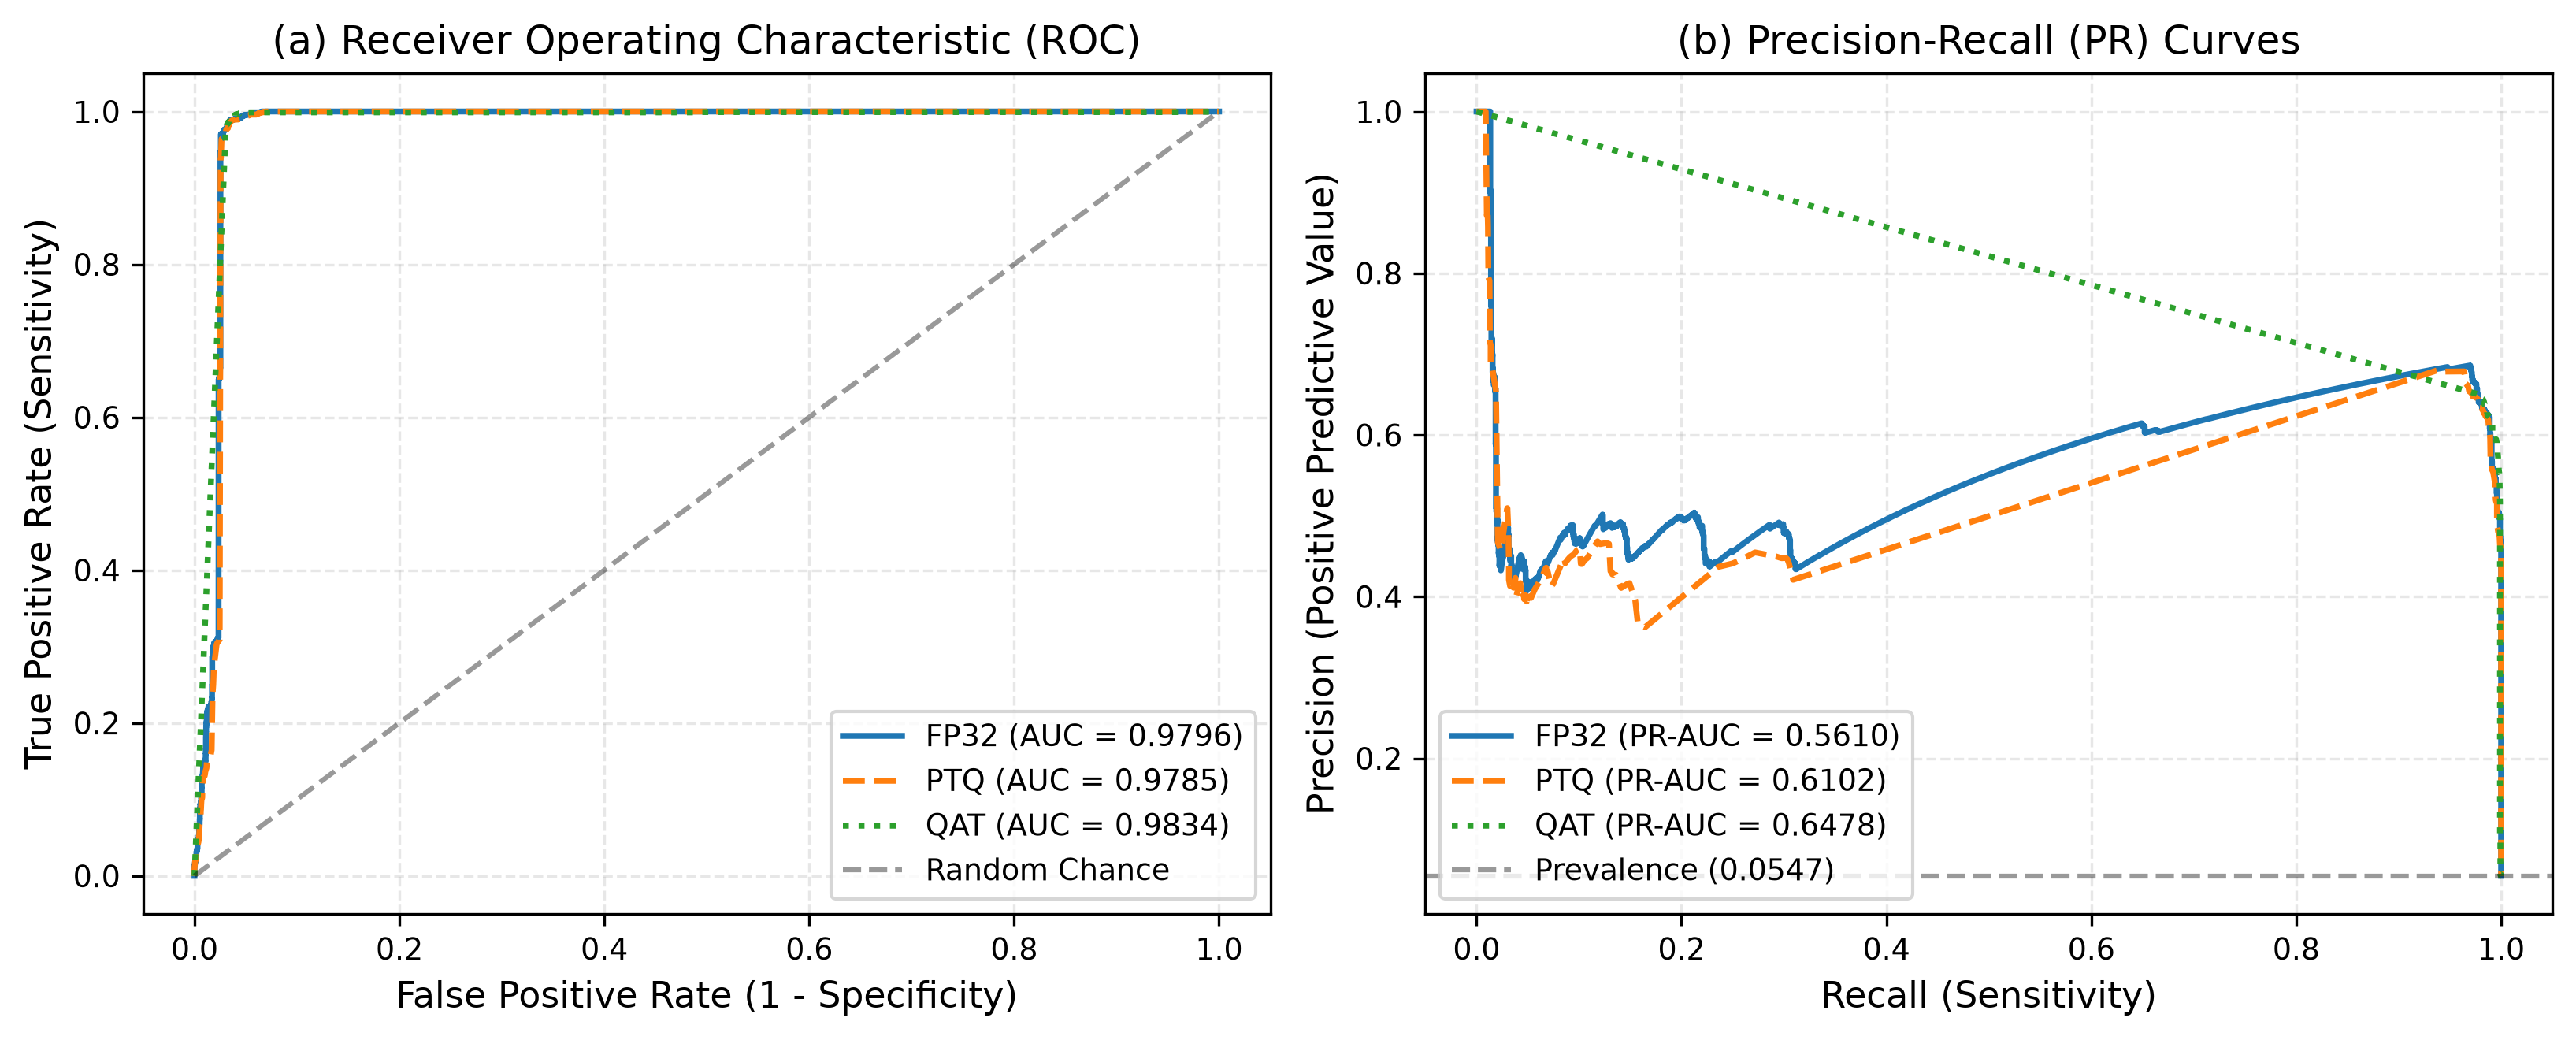
\includegraphics[width=\columnwidth]{figures/figure6_pr_curves.png}
\caption{Precision-recall curves across classification thresholds on the test partition ($N=49,251$). The horizontal dashed line denotes the empirical minority class prevalence ($5.47\%$). Primary quantization deployments (FP32, PTQ, QAT) are plotted for visual clarity; Table~\ref{tab:predictive} reports full metrics including the unquantized FP32-FT control.}
\label{fig:pr_curves}
\end{figure}

\begin{figure*}[htbp]
\centering
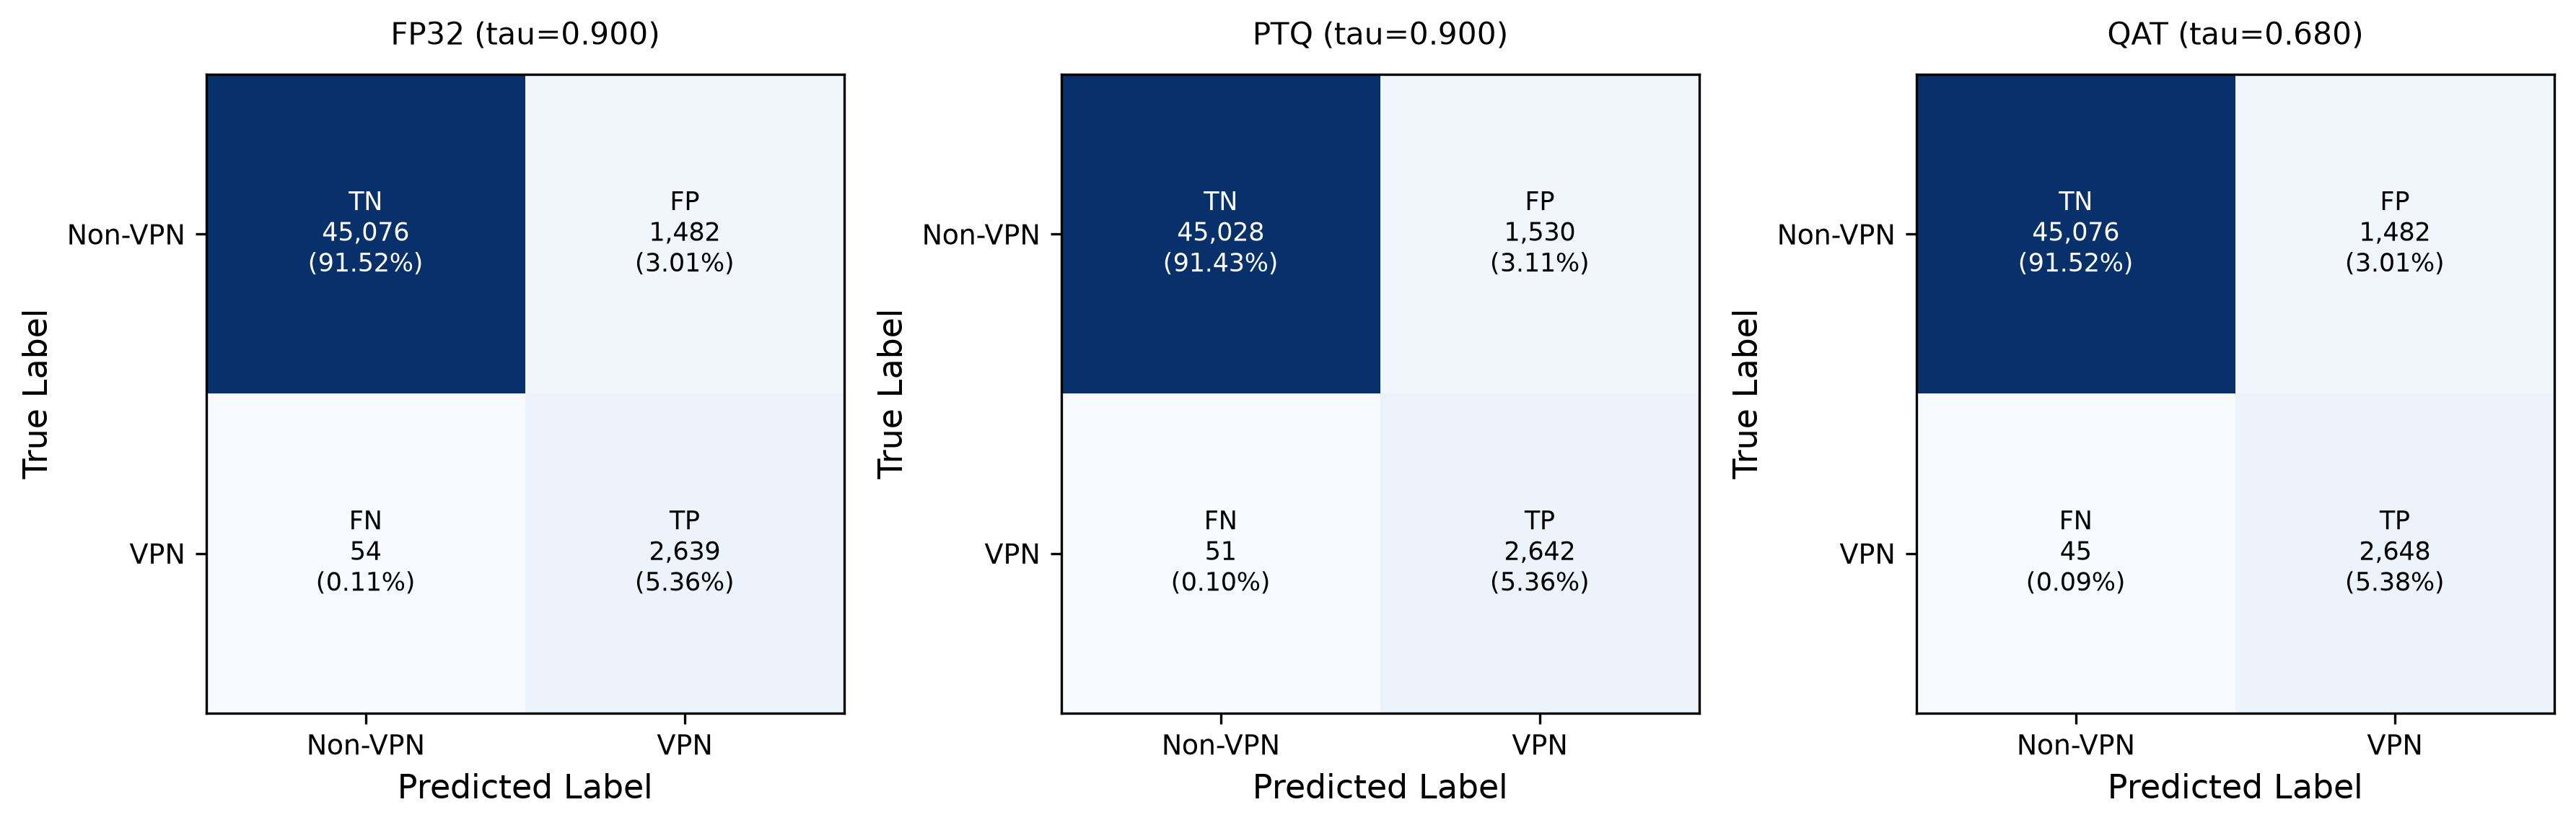
\includegraphics[width=\textwidth]{figures/figure4_confusion_matrices.png}
\caption{Confusion matrices on the held-out test partition ($N=49,251$) under model-specific calibrated operating thresholds ($\tau=0.900$ for FP32, $\tau=0.900$ for PTQ, and $\tau=0.680$ for QAT). Each cell reports the flow count and percentage share of total test traffic. Plotted for primary quantization deployments; Table~\ref{tab:predictive} reports complete 4-model performance.}
\label{fig:confusion_matrices}
\end{figure*}

\textbf{Threshold-Independent Ranking (Panel A):} Evaluated across all potential decision thresholds, all models demonstrate strong rank ordering. ROC-AUC values span a narrow band between 0.9785 and 0.9834. However, ROC-AUC is insensitive to minority detection errors in severe class imbalance. With 46,558 true negative flows, false alarm fluctuations alter the false positive rate denominator only marginally, leaving the ROC curve near the top-left boundary. 

Precision-Recall AUC (PR-AUC) provides a more direct measure of minority detection capability. As illustrated in Fig.~\ref{fig:pr_curves}, all models maintain precision well above the 0.0547 random prevalence line. Baseline FP32 scores a PR-AUC of 0.5610. PTQ improves this score to 0.6102 (+0.0492 gain), and QAT attains 0.6478 (+0.0868 gain). The unquantized fine-tuned control (FP32-FT) achieves 0.6128. Training noise introduced by fake-quantization operators during QAT acts as an effective regularizer, improving rank separation on ambiguous flows. Brier calibration scores reflect a parallel trend: QAT achieves the lowest mean squared prediction error (0.0237, compared to 0.0585 for FP32 and 0.0584 for PTQ).

\textbf{Calibrated Operating Performance (Panel B):} In active network deployments, an inspection engine must make hard binary decisions at a fixed threshold $\tau$. When thresholds are calibrated on the independent validation split ($\tau = 0.900$ for FP32, $\tau = 0.900$ for PTQ, $\tau = 0.680$ for QAT, and $\tau = 0.830$ for FP32-FT), all architectures demonstrate viable detection accuracy, as shown in the confusion matrices of Fig.~\ref{fig:confusion_matrices}.

INT8-PTQ reproduces the performance of the FP32 baseline with minimal variance. At the identical operating threshold of $\tau = 0.900$, PTQ achieves 96.79\% accuracy (a change of $-0.09\%$), identical balanced accuracy of 97.41\%, and 98.11\% VPN recall (+0.11\% gain), yielding an $F_1$-score of 0.7697 (compared to 0.7746 for baseline). Across the entire 49,251-flow evaluation set, PTQ induces only 57 prediction flips ($0.12\%$ of traffic), confirming that post-training quantization preserves the operational decision boundary when evaluated at the calibrated operating point.

Calibrated QAT achieves the highest balanced accuracy (97.57\%) and peak recall (98.33\%), correctly identifying 2,648 of 2,693 VPN flows while missing only 45 instances. Its calibrated $F_1$-score of 0.7762 slightly exceeds the FP32 baseline. The unquantized fine-tuned control (FP32-FT) attains the highest precision at 70.77\% and an $F_1$-score of 0.8176, indicating that additional training epochs refine boundary precision.

\textbf{The Threshold Transfer Failure (Panel C):} While QAT excels when calibrated, an operational failure occurs if an edge engineer deploys the quantized model while naively reusing the floating-point threshold ($\tau = 0.900$). 

Under PTQ, threshold reuse remains benign: positive calls increase by only 51 flows (4,172 vs. 4,121), balanced accuracy stays at 97.41\%, and the $F_1$-score remains 0.7697. For QAT, however, reusing the baseline threshold triggers a complete detection blackout. The uncalibrated QAT model emits zero positive calls across all 49,251 test flows (down from 4,121 positive calls in the baseline).

VPN recall falls to 0.00\%, the $F_1$-score drops to 0.0000, and balanced accuracy collapses to 50.00\% (the level of random guessing). Every single VPN flow in the test set is missed: 2,693 false negatives out of 2,693 true positive flows. A total of 4,121 flows flip from positive to negative, altering classifications across 8.37\% of all monitored traffic.

This result reveals a practical pitfall. In Panel A, QAT achieved the highest ROC-AUC (0.9834) and the highest PR-AUC (0.6478). Yet under direct threshold transfer in Panel C, it suffers total operational failure. Threshold transferability cannot be assumed when deploying quantized models, and post-quantization threshold calibration on validation data is strictly required.

\subsection{Mechanistic Proof of Output Saturation}

The complete minority-class failure of the QAT model under the uncalibrated baseline threshold ($\tau = 0.900$) is an arithmetic artifact of integer serialization rather than a failure of representation learning. While threshold-independent evaluations confirm that QAT separates traffic classes effectively (PR-AUC $= 0.6478$, ROC-AUC $= 0.9834$), the runtime conversion of the network bounds its dynamic range.

Under the QNNPACK execution engine on ARM64 hardware, the output linear layer (\texttt{fc2}) serializes into an unsigned 8-bit quantized representation with integer states $q_{\text{out}} \in \{0, 1, \dots, 255\}$. As formalized in (\ref{eq:dequant_out})--(\ref{eq:p_max}), the uniform affine dequantization operator fixes scale $s_{\text{out}} = 0.02535125$ and zero-point offset $zp_{\text{out}} = 215$. With $q_{\max} = 255$, the maximal reachable logit ceiling is strictly bounded at $z_{\max} = +1.014050$ (\ref{eq:z_max}), enforcing an absolute output probability ceiling of $p_{\max} = 0.733812$ (\ref{eq:p_max}). No network input, regardless of how distinctive its packet features may be, can produce an output probability exceeding $0.733812$ under this serialized operator.

\begin{figure}[htbp]
\centering
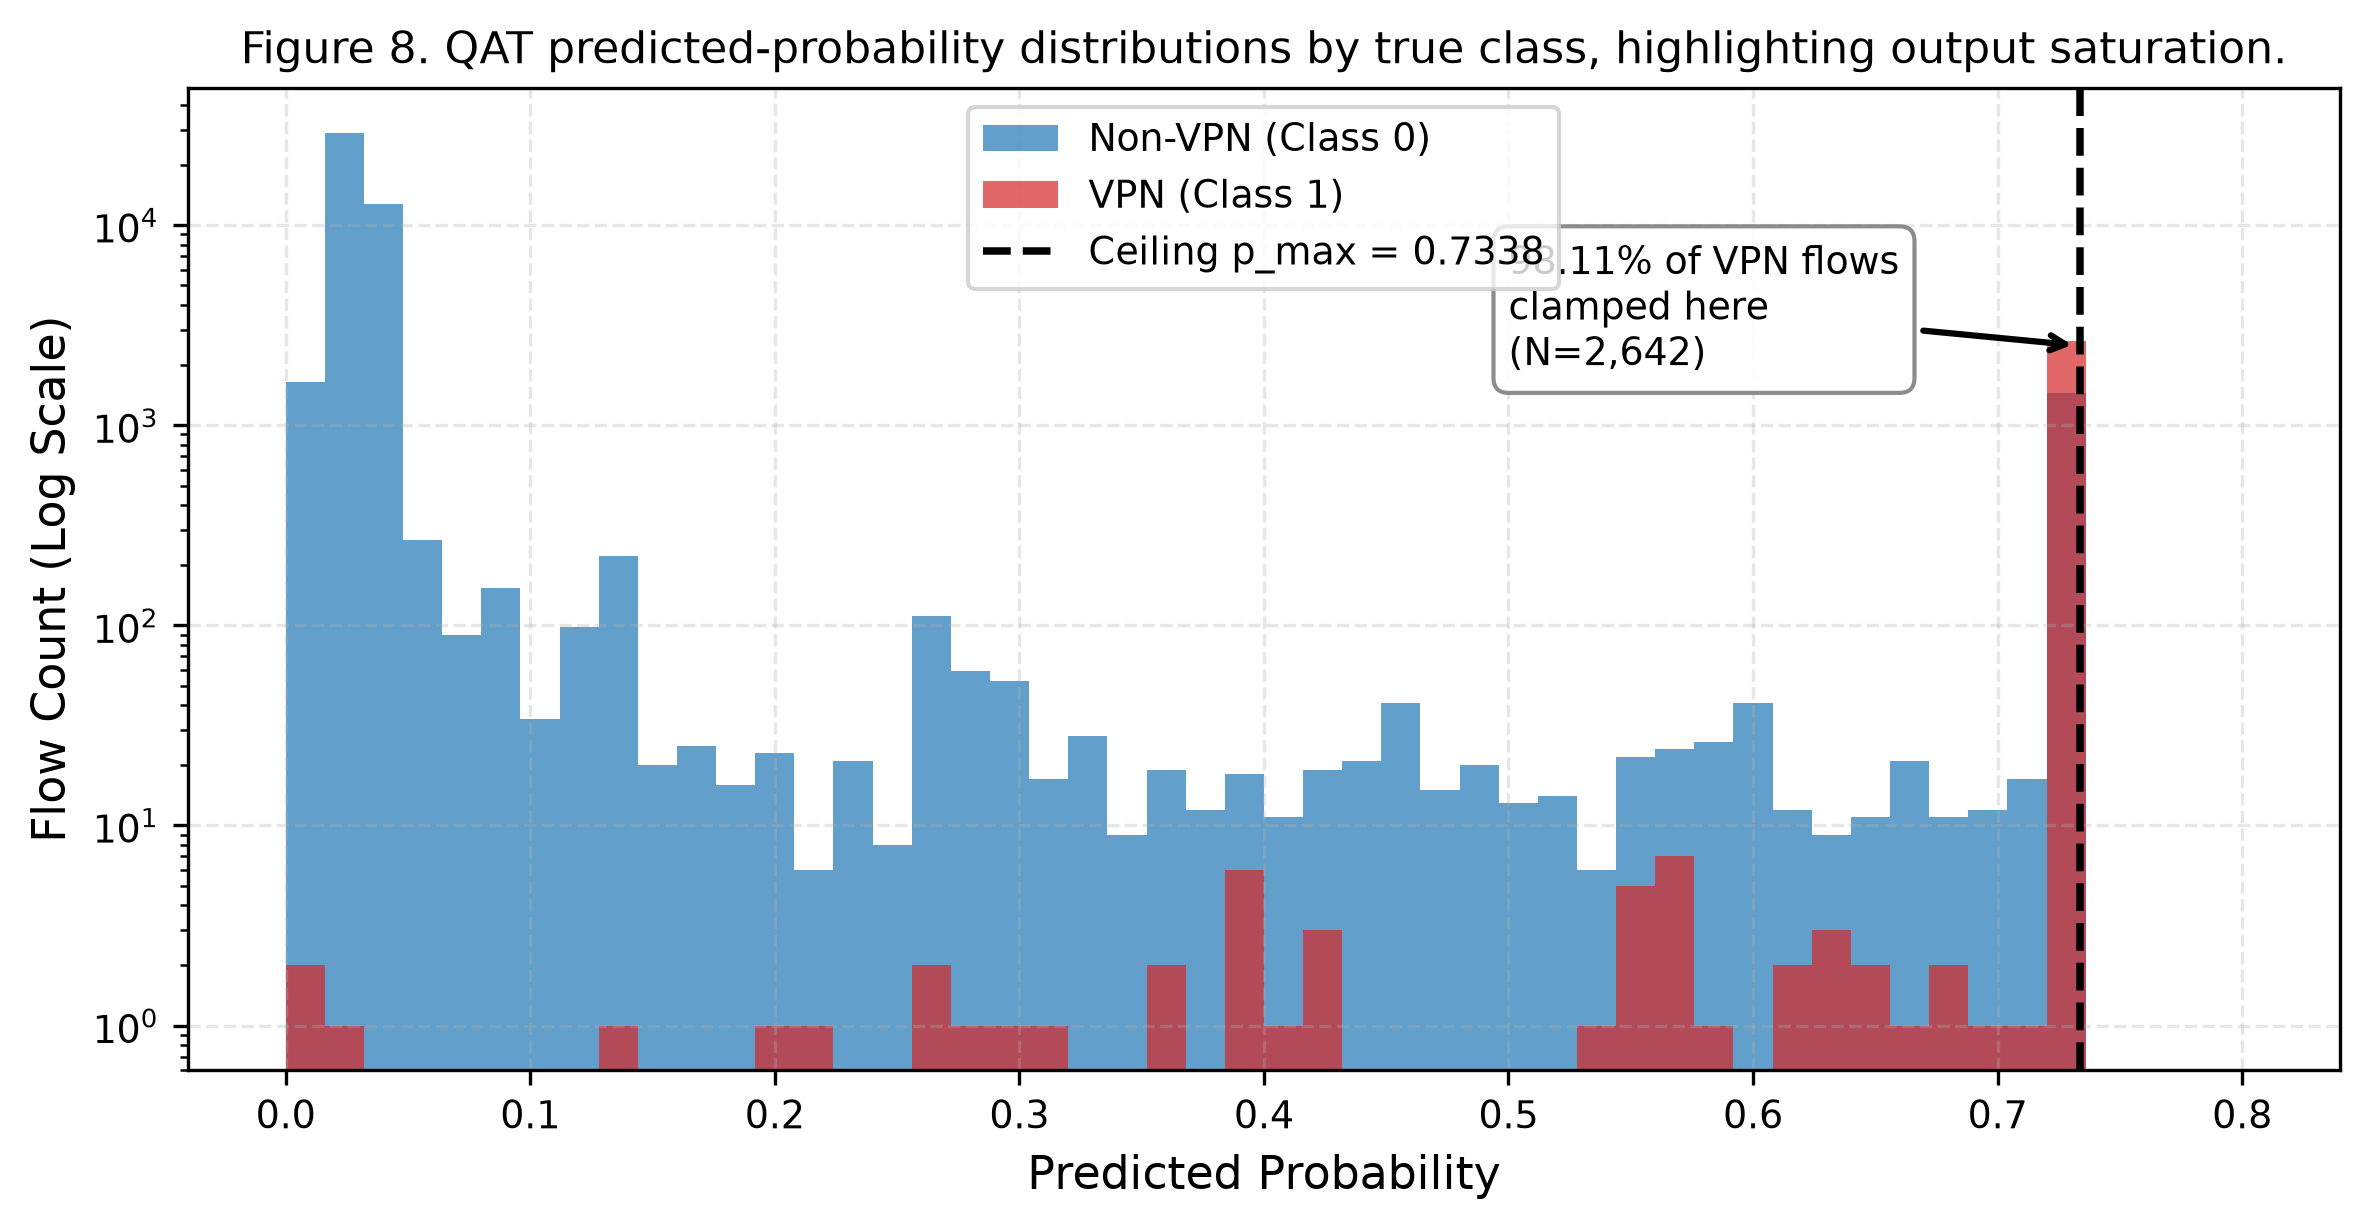
\includegraphics[width=\columnwidth]{figures/figure8_qat_probability_saturation.png}
\caption{Predicted probability distributions of the INT8-QAT model across 49,251 test flows by true class. The unsigned 8-bit quantization ceiling at $p_{\max} = 0.733812$ clamps 98.11\% (2,642 of 2,693) of all test VPN flows to an identical score. Probability bins above 0.74 remain completely empty.}
\label{fig:qat_saturation}
\end{figure}

Evaluating all 49,251 test flows reveals the direct operational consequence of this mathematical bound. Exactly 4,070 flows saturate at $p_{\max} = 0.73381203$. Of these saturated instances, 2,642 are true VPN flows, representing 98.11\% of the entire test VPN population (2,642 of 2,693 flows). Nearly all positive flows in the test partition pile up against this ceiling. As shown in Fig.~\ref{fig:qat_saturation}, the probability bins in $(0.74, 1.00]$ are completely vacant. Applying any operational threshold $\tau > 0.7338$ trivially yields zero positive detections, producing an $F_1$ score of exactly $0.0000$.

Static PTQ avoids this limitation. It maintains an unconstrained output projection spanning pre-sigmoid logits from $-7.278$ to $+10.398$, reaching probabilities up to $0.999969$ with zero clamped flows. Recalibrating the QAT operating threshold on validation data ($\tau^* = 0.680 < p_{\max}$) successfully restores peak detection performance ($F_1 = 0.7762$, recall $= 98.33\%$). Even so, saturation destroys confidence gradation among positive calls: 98.11\% of all true VPN test flows (2,642 of 2,693)---representing 99.77\% of all correctly detected true VPN flows under the calibrated operating threshold (2,642 of 2,648 true positive detections)---receive the exact same maximal probability score ($p_{\max} = 0.733812$), preventing network operators from ranking alerts by confidence.

\subsection{Feature Attribution Drift and Causal Disentanglement}

Top-line classification accuracy indicates whether a compressed model reaches the correct label, but it does not reveal how the model reaches that label. If quantization alters the input features that drive classification, an operator inspecting post-hoc explanations may rely on justifications that no longer reflect the true decision path.

To audit explanation stability, we apply KernelSHAP to pre-sigmoid logits across a stratified evaluation cohort of $N = 100$ held-out test flows (50 VPN, 50 Non-VPN). The explainer runs with 150 coalition evaluations per flow against 50 background reference flows sampled from the training partition. All zero-padding tokens are masked so that attribution values reflect only active packet bytes. 

Attribution drift is measured across four complementary dimensions:
\begin{enumerate}
    \item \textbf{Top-$k$ Intersection-over-Union ($IoU_k$):} The Jaccard similarity between the sets of $k$ largest attribution magnitudes in the FP32 baseline and the target model, evaluated at $k = 5$ and $k = 10$.
    \item \textbf{Total Variation Distance ($TV$):} The normalized attribution mass displacement, defined as $TV = \frac{1}{2} \sum_{i} |a_i^{\text{FP32}} - a_i^{\text{target}}|$, where $\sum_i |a_i| = 1$.
    \item \textbf{Signed Cosine Similarity ($S_c$):} The directional alignment between attribution vectors, given by $S_c = (\mathbf{a}^{\text{FP32}} \cdot \mathbf{a}^{\text{target}}) / (\|\mathbf{a}^{\text{FP32}}\|_2 \|\mathbf{a}^{\text{target}}\|_2)$.
    \item \textbf{Spearman Rank Correlation ($r_s$):} The monotonic rank ordering of feature attributions across the active packet sequence.
\end{enumerate}

Because sampling-based explainers contain stochastic variance, evaluating drift requires an empirical reference boundary. We establish this Explainer Noise Floor by executing KernelSHAP across three independent random seeds on the unchanged FP32 baseline model. This boundary captures the variance of the estimator itself: $IoU_5 = 0.9553 \pm 0.1829$, $IoU_{10} = 0.9648 \pm 0.1592$, $TV = 0.0553 \pm 0.1588$, $S_c = 0.9676 \pm 0.1450$, and $r_s = 0.9516 \pm 0.1666$. Metric shifts within these intervals cannot be distinguished from explainer sampling noise.

To isolate the cause of attribution changes during quantization-aware training, we also evaluate an unquantized fine-tuning control (FP32-FT). This control model is trained with the exact same 5-epoch AdamW schedule ($lr = 10^{-4}$) as QAT, but retains full 32-bit floating-point weights and activations without quantization layers.

\begin{table*}[htbp]
\caption{Feature Attribution Drift and Explainer Repeatability ($N=100$ Test Cohort)}
\label{tab:attribution}
\centering
\begin{tabular}{lccccc}
\toprule
\textbf{Condition / Comparison} & \textbf{Top-5 IoU} & \textbf{Top-10 IoU} & \textbf{Total Variation ($TV$)} & \textbf{Signed Cosine ($S_c$)} & \textbf{Spearman ($r_s$)} \\
\midrule
Combinatorial Random Chance & 0.0220 & 0.0426 & --- & 0.0000 & 0.0000 \\
Explainer Noise Floor (FP32 Multi-Seed) & $0.9553 \pm 0.1829$ & $0.9648 \pm 0.1592$ & $0.0553 \pm 0.1588$ & $0.9676 \pm 0.1450$ & $0.9516 \pm 0.1666$ \\
FP32 vs. FP32-FT (Fine-Tuning Control) & $0.9669 \pm 0.1375$ & $0.9762 \pm 0.1169$ & $0.1219 \pm 0.1137$ & $\mathbf{0.9554 \pm 0.0953}$ & $0.9687 \pm 0.1092$ \\
FP32 vs. INT8-PTQ & $\mathbf{0.9786 \pm 0.0970}$ & $\mathbf{0.9887 \pm 0.0650}$ & $\mathbf{0.0369 \pm 0.0620}$ & $\mathbf{0.9918 \pm 0.0394}$ & $\mathbf{0.9749 \pm 0.0592}$ \\
FP32 vs. INT8-QAT & $0.9553 \pm 0.1841$ & $0.9679 \pm 0.1416$ & $0.2346 \pm 0.1908$ & $\mathbf{0.4830 \pm 0.3449}$ & $0.9140 \pm 0.1838$ \\
\bottomrule
\end{tabular}
\end{table*}

\begin{figure}[htbp]
\centering
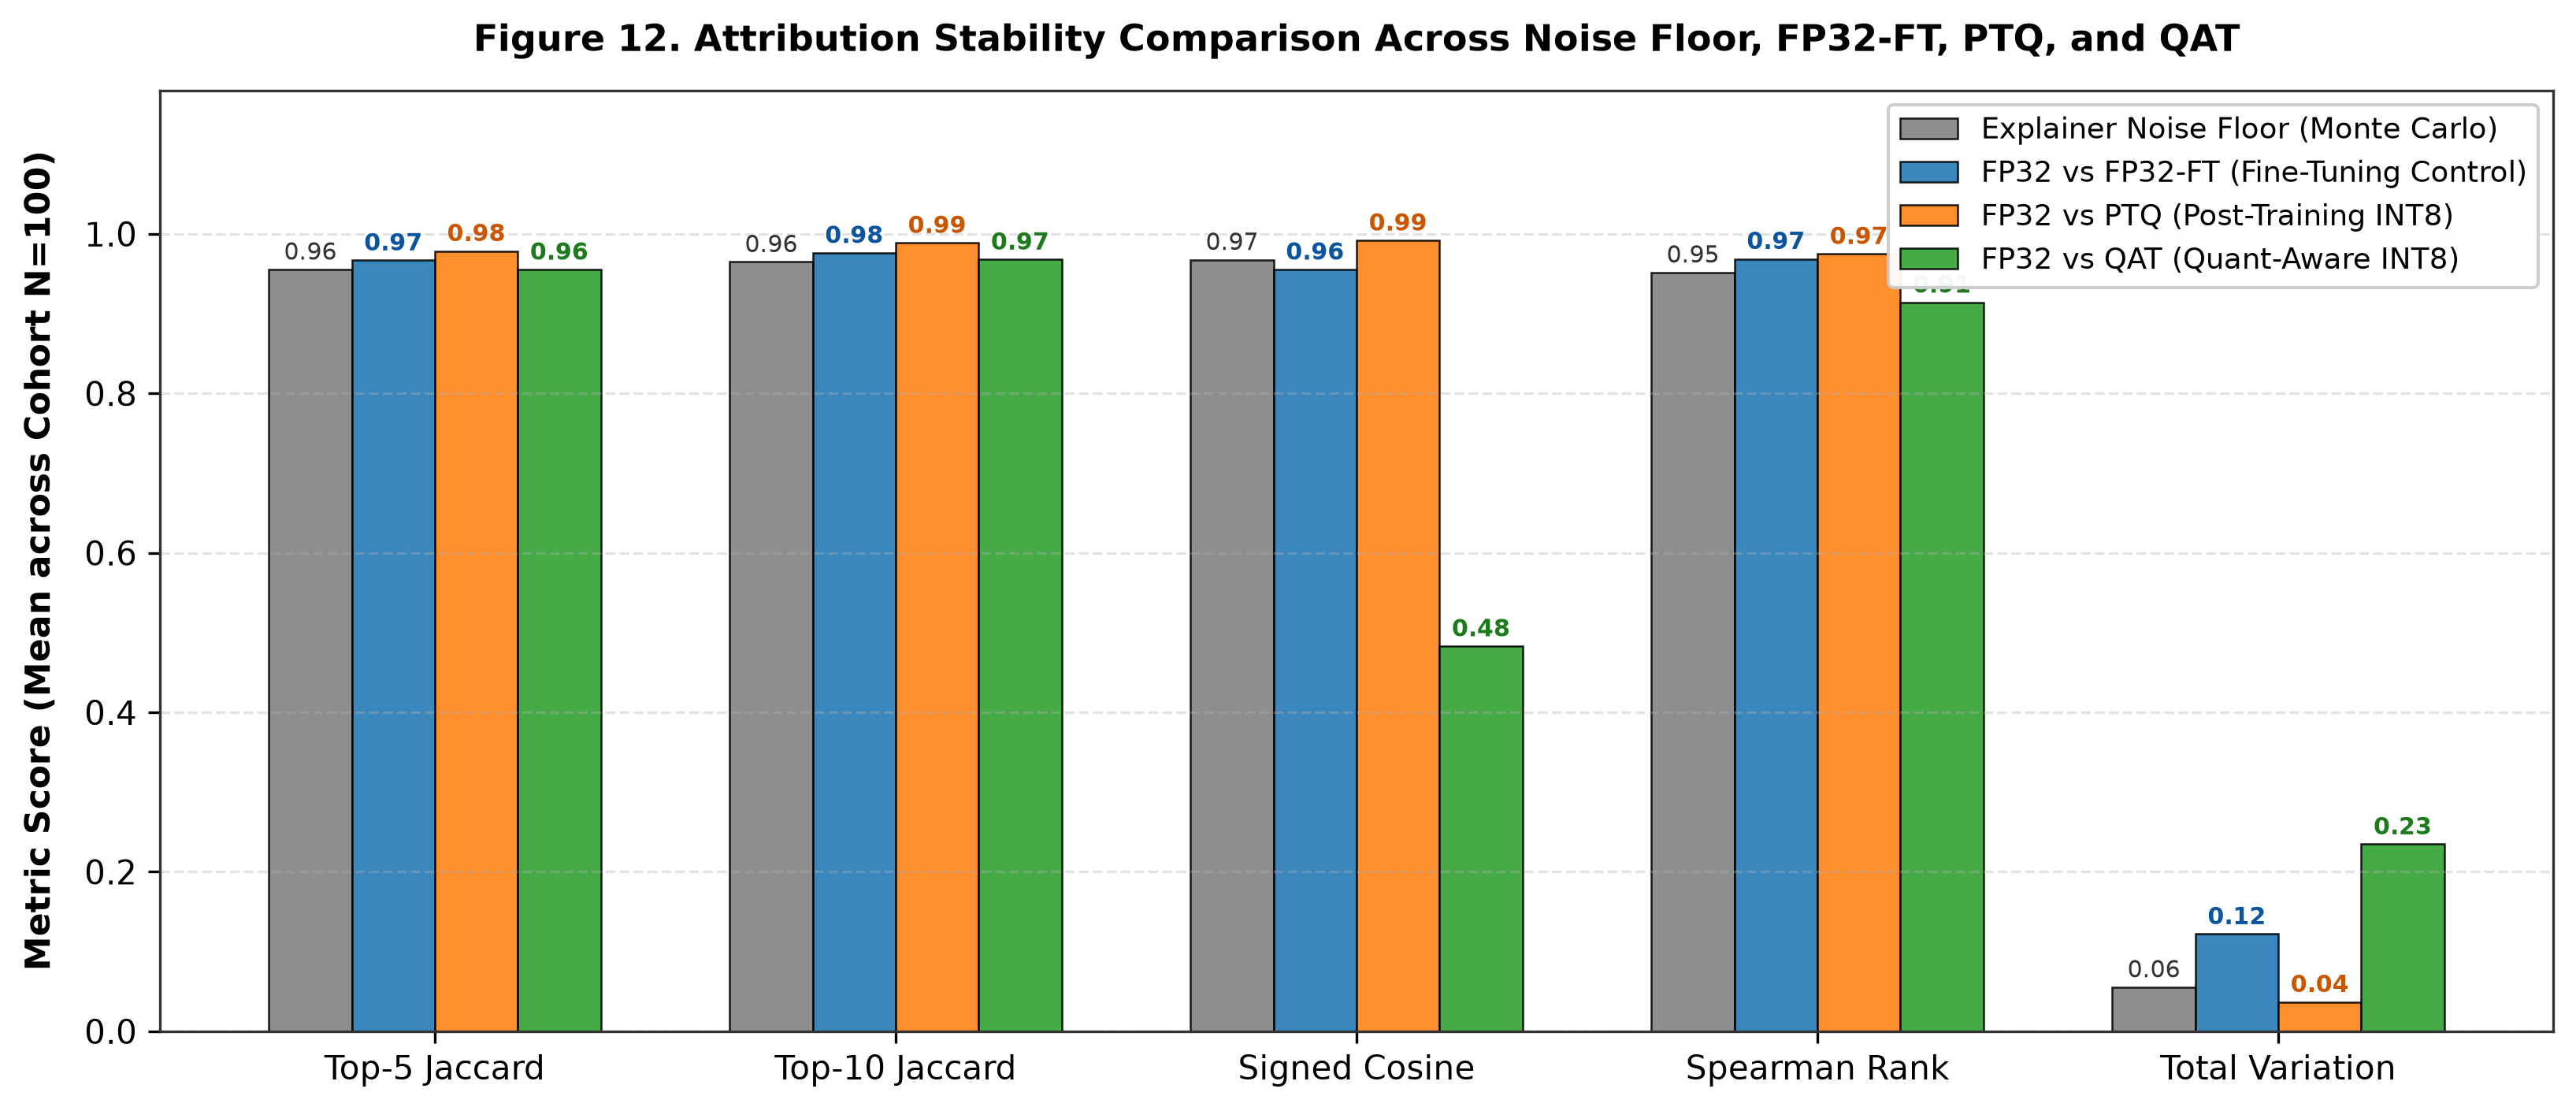
\includegraphics[width=\columnwidth]{figures/figure12_attribution_stability_comparison.png}
\caption{Feature attribution stability metrics across the $N=100$ test cohort. FP32-FT and INT8-PTQ preserve directional alignment with the baseline ($S_c = 0.9554$ and $0.9918$, respectively), whereas INT8-QAT exhibits directional collapse ($S_c = 0.4830$) alongside an elevated Total Variation distance ($TV = 0.2346$).}
\label{fig:attribution_stability}
\end{figure}

Table~\ref{tab:attribution} and Fig.~\ref{fig:attribution_stability} report the quantitative attribution comparisons across the test cohort. The measurements establish four primary findings:

\textbf{1) PTQ Preserves Baseline Logic:} Static PTQ maintains near-perfect alignment with the uncompressed model. In 95 of the 100 test flows, PTQ selects the exact same Top-5 features as the FP32 baseline ($IoU_5 = 0.9786 \pm 0.0970$). Directional similarity remains high at $S_c = 0.9918 \pm 0.0394$, and attribution redistribution is low ($TV = 0.0369 \pm 0.0620$). A paired Wilcoxon signed-rank test against the noise floor detects a small rank displacement ($W = 1506.0$, $p = 0.000459$), but the median change in Total Variation distance is minimal ($\text{median } \Delta TV = +0.0049$). For static quantization, explanations generated from the uncompressed model transfer reliably to the quantized deployment.

\textbf{2) Causal Disentanglement via FP32-FT:} A key question is whether attribution changes in QAT originate from parameter fine-tuning or from discrete quantization constraints. The FP32-FT control resolves this question. Without quantization layers, fine-tuning preserves directional alignment ($S_c = 0.9554 \pm 0.0953$), tracking the noise floor ($0.9676$) and PTQ ($0.9918$). Feature selection stability remains equally high ($IoU_5 = 0.9669 \pm 0.1375$, $IoU_{10} = 0.9762 \pm 0.1169$). While unquantized fine-tuning shifts feature weights across the loss surface to induce moderate displacement ($TV = 0.1219 \pm 0.1137, W = 821.0, p = 4.66 \times 10^{-9}$ vs. noise floor), INT8-QAT incurs substantially steeper representational restructuring ($TV = 0.2346 \pm 0.1908$, Wilcoxon $W = 1146.0, p = 2.12 \times 10^{-6}$ vs. FP32-FT). In parallel, while FP32-FT preserves directional alignment ($S_c = 0.9554 \pm 0.0953$), INT8-QAT induces severe directional collapse ($S_c = 0.4830 \pm 0.3449$ overall, collapsing to $S_c = 0.1665 \pm 0.1406$ on minority VPN flows). This demonstrates a two-stage causal mechanism: stochastic gradient descent fine-tuning induces initial feature reallocation across an overparameterized loss surface, but discrete integer quantization constraints and Straight-Through Estimator (STE) gradient approximations inject an additional, severe representational disruption.

\textbf{3) Directional Collapse Under QAT:} While QAT retains broad feature overlap ($IoU_5 = 0.9553 \pm 0.1841$, $IoU_{10} = 0.9679 \pm 0.1416$) and general rank ordering ($r_s = 0.9140 \pm 0.1838$), its directional alignment breaks down completely. Signed cosine similarity plunges to $S_c = 0.4830 \pm 0.3449$ ($p < 10^{-17}$ compared to both PTQ and FP32-FT), while Total Variation distance increases to $TV = 0.2346 \pm 0.1908$. The model still attends to similar token regions, but it redistributes attribution weights and reverses their polarities. An explanation from the FP32 baseline cannot be assumed to describe the reasoning of the QAT model.

\textbf{4) Class-Conditional Attribution Asymmetry:} Evaluating drift separately across traffic classes reveals an asymmetric distribution. On Non-VPN flows, QAT preserves moderate directional alignment ($S_c = 0.7996 \pm 0.1360$), with drift manifesting primarily as magnitude scaling ($TV = 0.3529 \pm 0.0691$). On VPN flows, directional alignment collapses almost entirely, dropping to $S_c = 0.1665 \pm 0.1406$ (median $0.1341$), while attribution mass remains more concentrated ($TV = 0.1163 \pm 0.2025$). A Mann-Whitney $U$ test on signed cosine similarity confirms that minority VPN flows suffer substantially steeper directional degradation than Non-VPN traffic ($U = 89.0$, $p = 1.24 \times 10^{-15}$). Conversely, a separate Mann-Whitney $U$ test on Total Variation distance confirms that Non-VPN flows exhibit markedly higher overall attribution mass displacement ($U = 278.0$, $p = 2.12 \times 10^{-11}$). For obfuscated tunneling traffic, the quantized model relies on fundamentally rearranged combinations of feature polarities to reach its classifications.

\subsection{Clustered Statistical Inference and Non-IID Session Dynamics}

Network traffic classification datasets do not consist of independent and identically distributed (IID) samples. Flows generated during a single capture session share operating system network stacks, congestion control state, packet fragmentation boundaries, and temporal background noise. Treating each flow as an independent observation commits a pseudo-replication fallacy. When we evaluate the 49,251 held-out test flows with a standard paired $t$-test comparing uncompressed FP32 and INT8-PTQ pre-sigmoid logits, the test yields $t = -38.93$ ($p < 10^{-300}$). Such an extreme test statistic appears to indicate that PTQ systematically depresses classification logits. However, that result is an artifact of treating clustered observations as independent trials, which deflates the estimated standard error by a factor of 56.

\begin{table}[htbp]
\caption{Canonical Test Session Breakdown and Logit Shifts ($K=16$)}
\label{tab:session_shifts}
\centering
\scriptsize
\setlength{\tabcolsep}{2pt}
\begin{tabular}{lcrrcc}
\toprule
\textbf{Session Group} & \textbf{Class} & \textbf{Flows} & \textbf{Share} & \textbf{Mean $\Delta z$} & \textbf{Std} \\
\midrule
\texttt{skype\_audio3} & Non-VPN & 39,179 & 79.55\% & $-0.1164$ & 0.2303 \\
\texttt{email1} & Non-VPN & 5,727 & 11.63\% & $-0.0543$ & 0.2652 \\
\texttt{vpn\_hangouts\_audio2} & VPN & 2,135 & 4.33\% & $+0.3124$ & 0.1689 \\
\texttt{email2} & Non-VPN & 581 & 1.18\% & $+0.4209$ & 0.3210 \\
\texttt{vpn\_bittorrent} & VPN & 406 & 0.82\% & $-0.7204$ & 3.8659 \\
\texttt{voipbuster1} & Non-VPN & 398 & 0.81\% & $+0.2785$ & 0.2744 \\
\textit{10 Remaining} & Mixed & 825 & 1.68\% & $+0.10$ to $+0.53$ & 0.22--0.41 \\
\midrule
\textbf{Pooled Test Partition} & Mixed & \textbf{49,251} & \textbf{100.0\%} & \textbf{$-0.0778$} & \textbf{0.4437} \\
\bottomrule
\end{tabular}
\end{table}

To analyze the behavior across independent communication events, we group the test partition into its $K = 16$ canonical session clusters. Table~\ref{tab:session_shifts} summarizes the sample sizes, traffic proportions, and logit shift distributions across these sessions. The partition exhibits severe volume concentration: a single session, \texttt{skype\_audio3}, contains 39,179 flows, or 79.55\% of the test cohort. In that session, PTQ reduces logits, producing a mean shift of $-0.1164$ ($\sigma = 0.2303$). In contrast, 13 of the 16 canonical sessions (81.25\%) exhibit positive logit shifts, ranging from $+0.1037$ in \texttt{icqchat1} to $+0.5262$ in \texttt{netflix2}. Only three sessions show negative mean shifts: \texttt{skype\_audio3} ($-0.1164$), \texttt{email1} ($-0.0543$), and \texttt{vpn\_bittorrent} ($-0.7204$).

\begin{figure}[htbp]
\centering
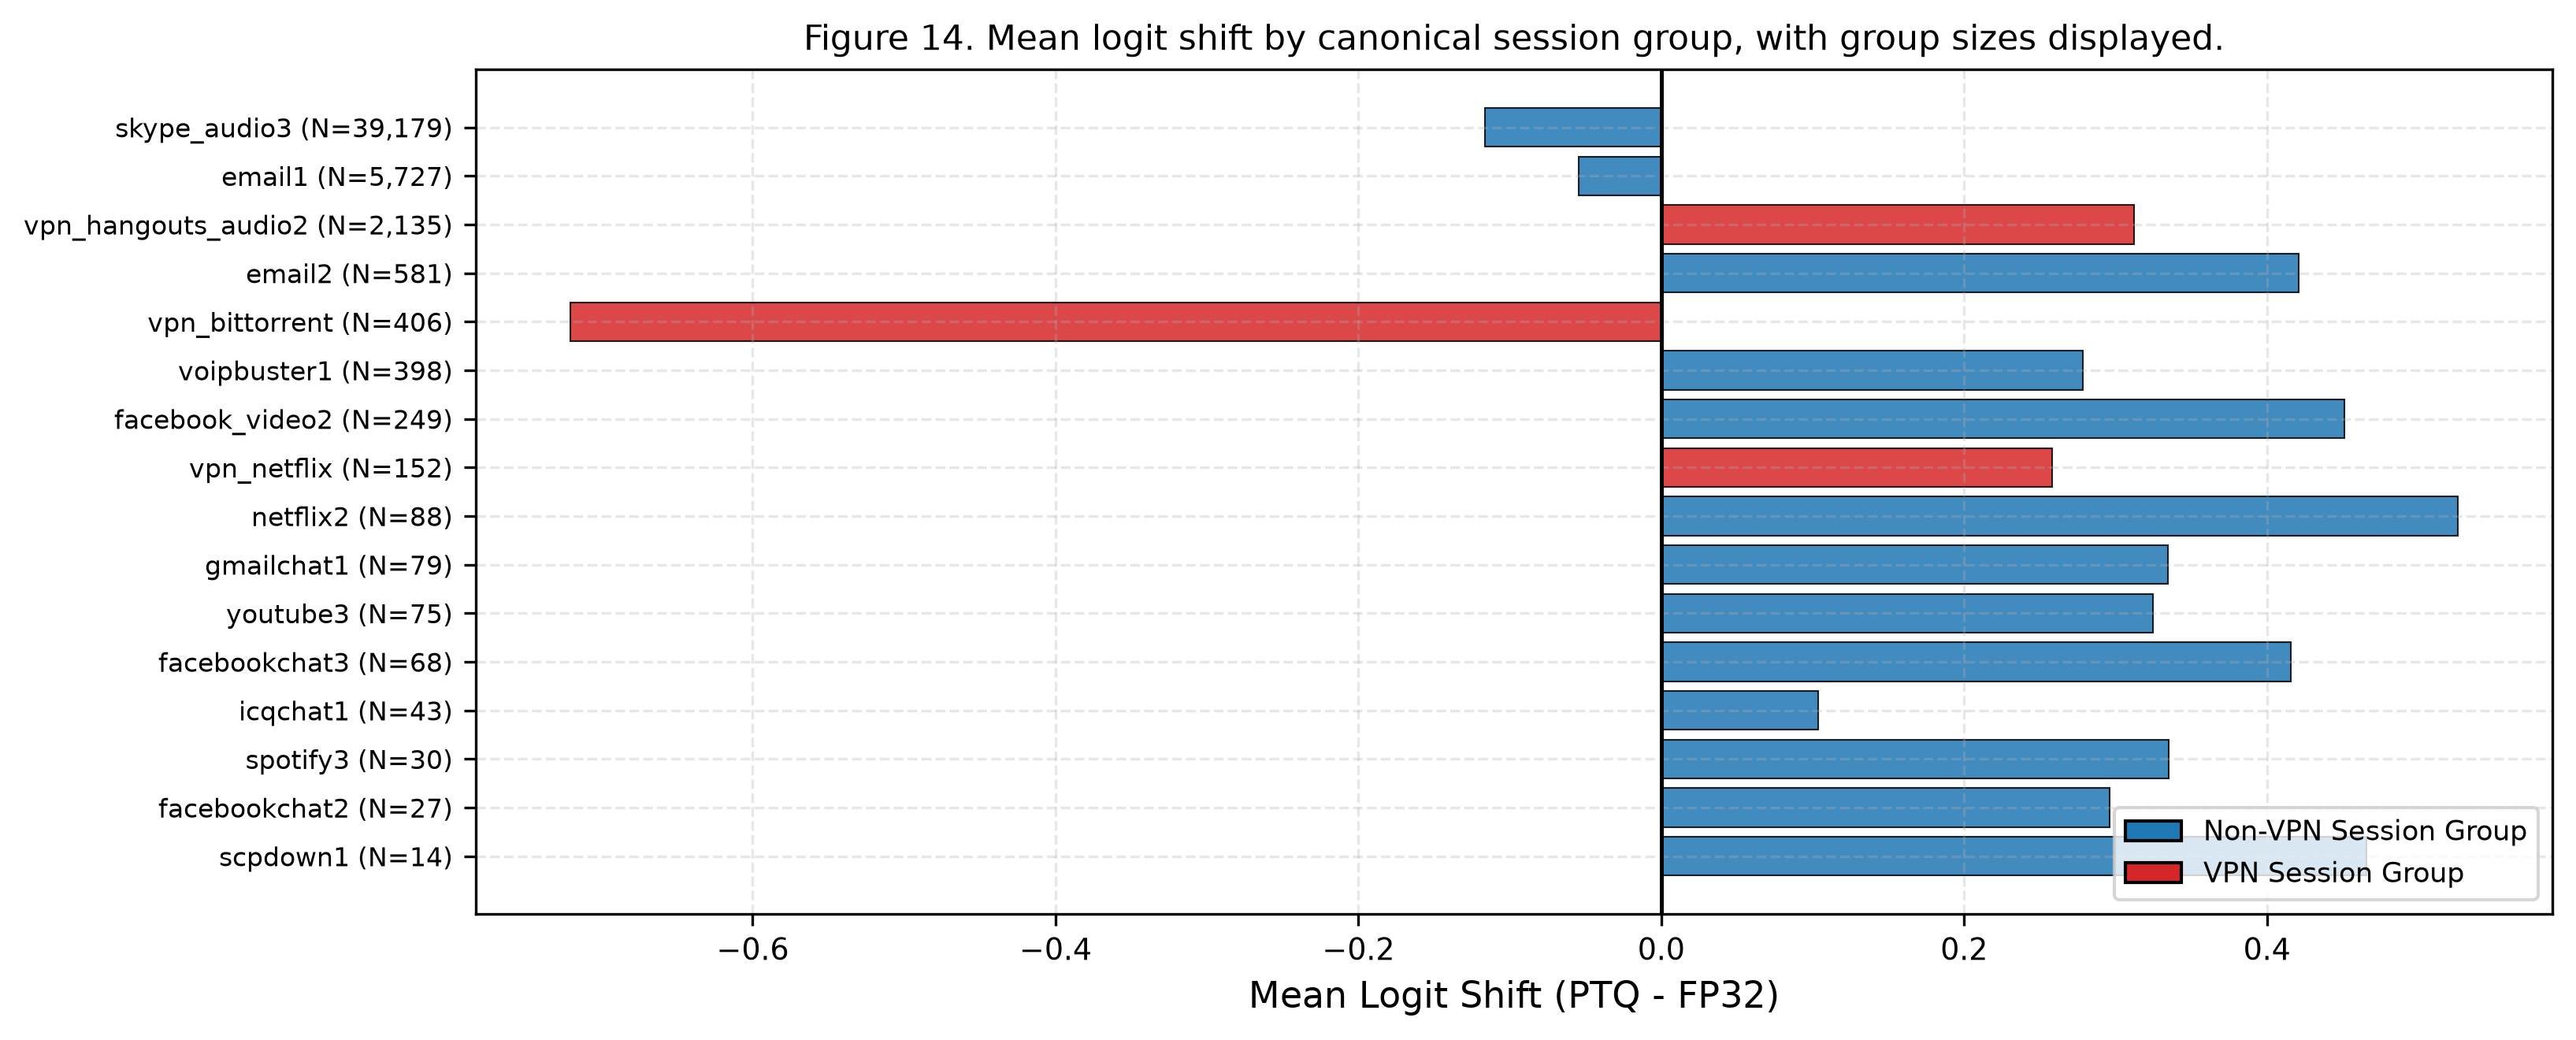
\includegraphics[width=\columnwidth]{figures/figure14_group_logit_shifts.png}
\caption{Mean PTQ logit shift ($\Delta z = z_{\text{PTQ}} - z_{\text{FP32}}$) across the 16 canonical test sessions. Although 13 of 16 sessions (81.25\%) display positive shifts, the single high-volume session \texttt{skype\_audio3} ($N=39,179$) shifts negative, pulling the pooled flow average below zero.}
\label{fig:group_logit_shifts}
\end{figure}

Figure~\ref{fig:group_logit_shifts} shows this divergence across sessions. Thirteen horizontal bars extend into positive territory. Yet because the top session accounts for nearly four-fifths of the evaluation data, the pooled average is dragged negative to $-0.0778$. This dynamic represents an ecological reversal and an empirical case of Simpson's Paradox: the directional effect observed in the pooled aggregate directly reverses the effect present across most independent sub-populations.

To formalize this disparity, we define two distinct statistical estimands:
\begin{align}
\theta_A &= \frac{\sum_{k=1}^K \sum_{i=1}^{n_k} \Delta z_{k,i}}{\sum_{k=1}^K n_k} = -0.0778, \\
\theta_B &= \frac{1}{K} \sum_{k=1}^K \overline{\Delta z}_k = +0.2270,
\end{align}
where $\Delta z_{k,i}$ is the logit shift for flow $i$ in session $k$, and $\overline{\Delta z}_k$ is the session mean shift. Estimand A evaluates the flow-weighted pooled mean. It answers an operational question: what is the net logit displacement across all flows in this specific captured dataset? Estimand B evaluates the unweighted macro-mean across sessions. It answers an inductive question: what is the expected logit displacement when deploying the model to a new, unseen network session?

\begin{figure}[htbp]
\centering
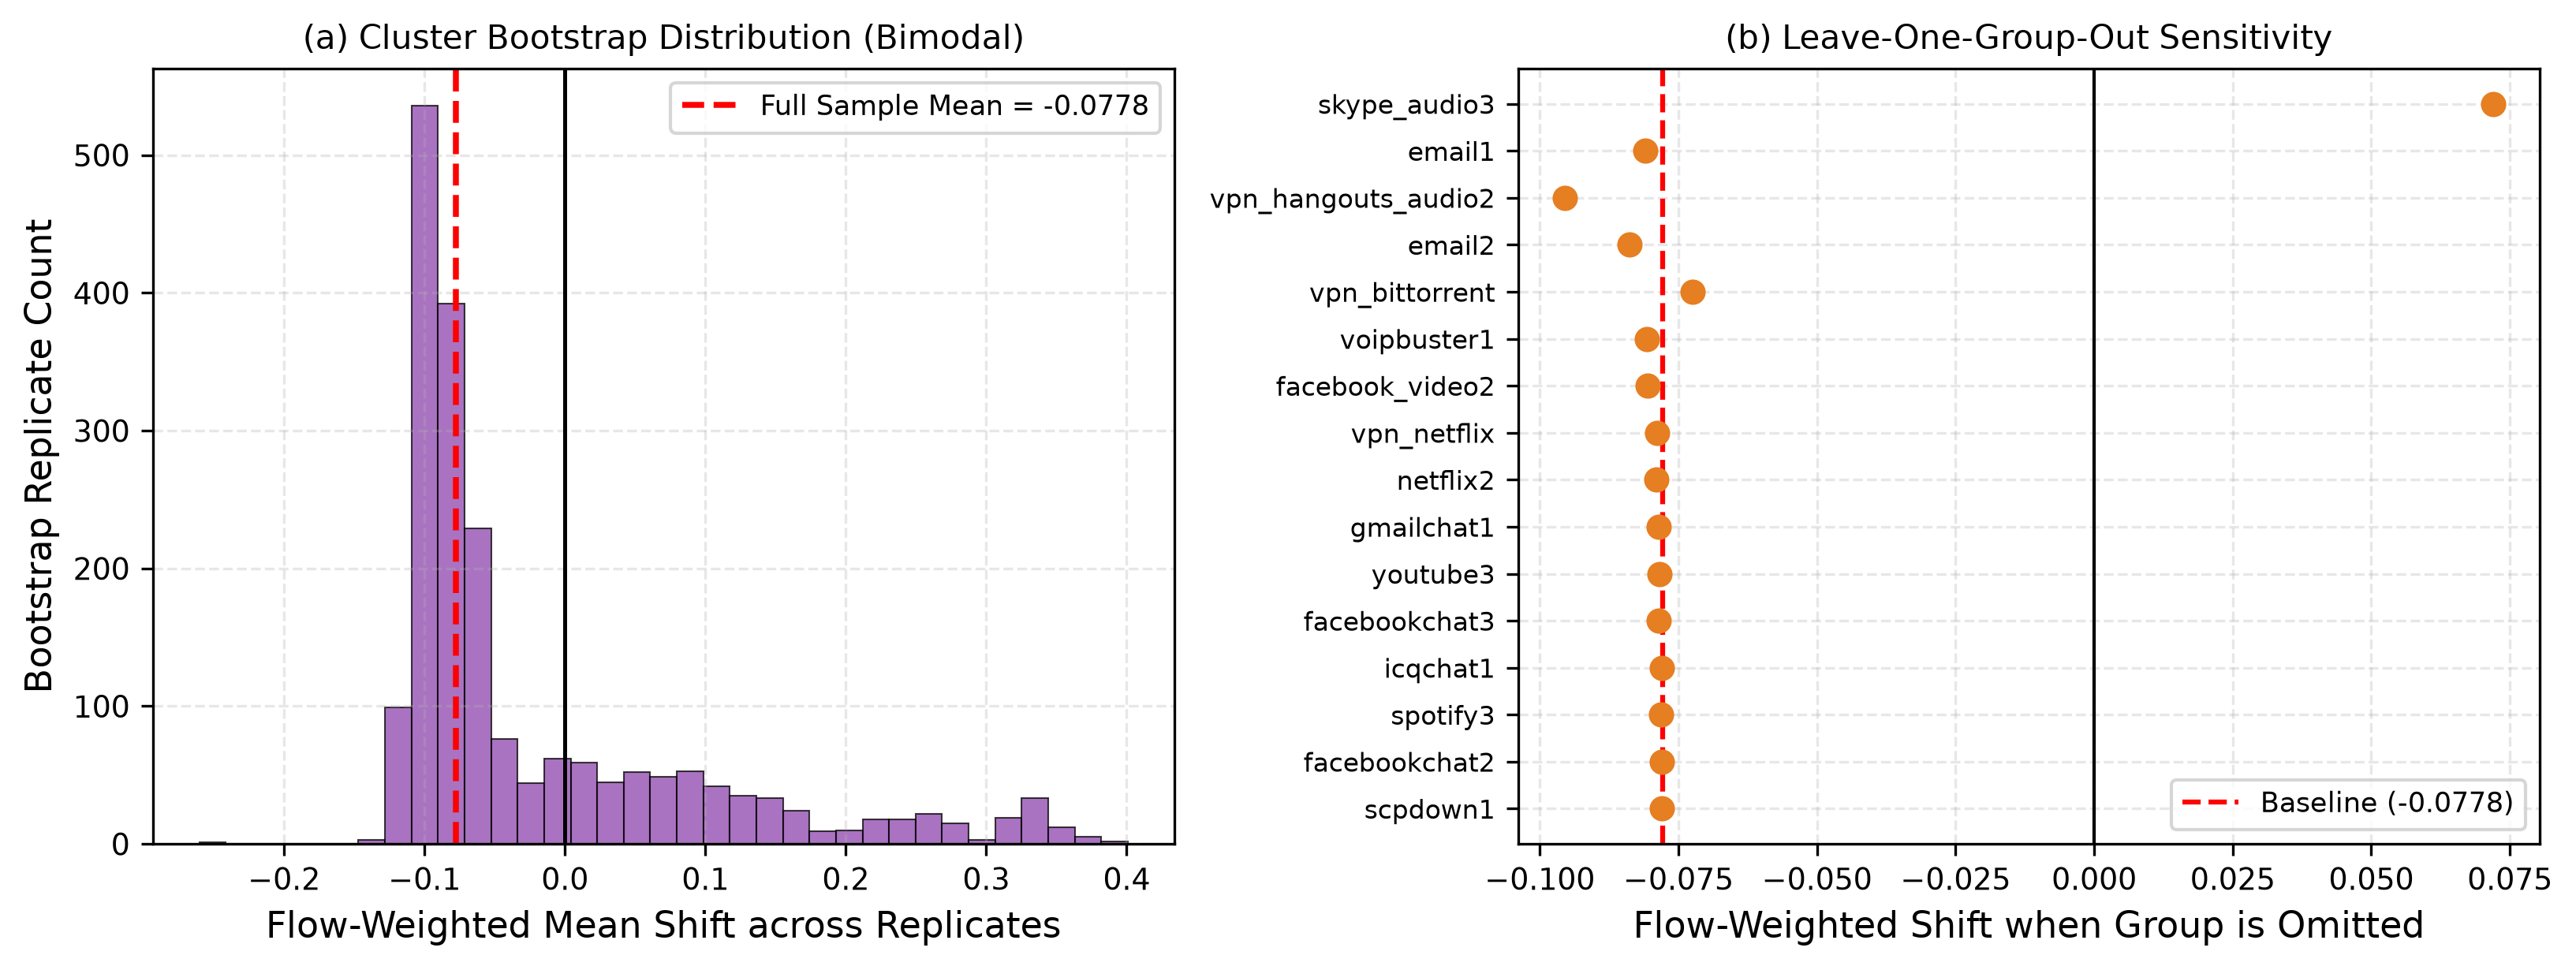
\includegraphics[width=\columnwidth]{figures/figure15_cluster_bootstrap_distribution.png}
\caption{Empirical distribution of Estimand A across 2,000 cluster bootstrap resamples. The distribution splits into two modes depending on whether \texttt{skype\_audio3} is selected, yielding a 95\% confidence interval ($[-0.1124, +0.3275]$) that spans zero.}
\label{fig:cluster_bootstrap}
\end{figure}

We compute confidence intervals using cluster bootstrap resampling with replacement across the 16 canonical sessions ($B = 2,000$ iterations, seed 42). For Estimand A, the cluster bootstrap produces a 95\% confidence interval of $[-0.1124, +0.3275]$ (and $[-0.1128, +0.3243]$ with 10,000 resamples). Because this interval spans zero, the pooled negative shift is not statistically distinguishable from zero once session clustering is recognized. For Estimand B, the cluster bootstrap produces a 95\% confidence interval of $[+0.0630, +0.3554]$ (and $[+0.0653, +0.3532]$ with 10,000 resamples), which is strictly positive and bounded away from zero.

Figure~\ref{fig:cluster_bootstrap} explains why the confidence interval for Estimand A is wide and asymmetric. The replicate distribution is distinctly bimodal rather than normal. The probability of drawing \texttt{skype\_audio3} at least once in a bootstrap sample of $K = 16$ clusters selected with replacement is:
\begin{equation}
P(\texttt{skype\_audio3} \in \text{sample}) = 1 - \left(1 - \frac{1}{K}\right)^K = 1 - \left(\frac{15}{16}\right)^{16} \approx 64.39\%.
\label{eq:skype_prob}
\end{equation}
In the 64.39\% of bootstrap draws where \texttt{skype\_audio3} appears, its 39,179 flows anchor the weighted average, centering replicate values between $-0.11$ and $-0.07$. In the remaining 35.61\% of draws where \texttt{skype\_audio3} is omitted, the remaining 15 sessions govern the calculation. Because 13 of those 15 sessions have positive means, the replicate average shifts upward, forming the secondary distribution between $+0.05$ and $+0.35$.

A leave-one-group-out (LOGO) sensitivity analysis confirms this concentration. Removing \texttt{skype\_audio3} from the test partition flips the pooled flow-weighted mean from $-0.0778$ to $+0.0720$. In contrast, removing any of the other 15 sessions leaves the pooled mean essentially unchanged, between $-0.0725$ and $-0.0955$. The apparent negative logit shift is an ecological artifact of one capture file. Treating packet flows as independent observations conceals this dependency, yielding false statistical certainty. Clustered inference is required to reflect session-level dynamics in quantized traffic models.

\section{Discussion}
Predictive stability does not imply representational fidelity. Task metrics hide internal distortions. While edge compression literature routinely validates quantized models solely through task-level discrimination metrics such as macro F1 or receiver operating characteristics \cite{b6}, \cite{b18}, fixed-point integer execution introduces unmonitored distortions across internal feature spaces. Attribution geometries can diverge sharply even when validation accuracy remains completely unaffected. Models arrive at correct classifications through entirely corrupted reasoning pathways. Below, we dissect the mathematical origins of this disconnect, demonstrate how integer saturation breaks automated security orchestration, analyze low-level ARM64 vector execution, examine legal compliance barriers, formalize session dependency structures, outline experimental limitations, and specify a concrete operational deployment protocol.

\subsection{Predictive Invariance versus Representational Reorganization}
Macroscopic predictive fidelity can completely decouple from microscopic attribution stability. The numbers reveal an unexpected fracture. When evaluating top-line performance on the leakage-free, session-isolated test partition ($N = 49,251$ flows), the uncompressed FP32 baseline attains a VPN-class $F_1$ of $0.7746$, an overall accuracy of $96.88\%$ ($0.9688$), and an ROC-AUC of $0.9796$, with a parameter footprint of $184.24\text{ KB}$. Converting weights to static Post-Training Quantization (INT8-PTQ) compresses the model footprint to $51.81\text{ KB}$—a $3.56\times$ compression ratio approaching the theoretical $4.0\times$ integer limit—while maintaining predictive invariance: VPN-class $F_1$ is $0.7697$, accuracy is $96.79\%$ ($0.9679$), and ROC-AUC is $0.9785$. Internal feature attribution geometry remains preserved. Signed cosine similarity reaches $S_c = 0.9918$. Top-5 feature Intersection-over-Union hits $\text{IoU}_5 = 0.9786$, with 95 out of 100 evaluated audit flows retaining strictly identical Top-5 features. PTQ maintains representational fidelity.

Quantization-Aware Training (INT8-QAT) presents an inverse behavioral profile. Outward gains mask severe internal drift. Under its recalibrated decision threshold ($\tau_{\text{cal}} = 0.680$), INT8-QAT yields a VPN-class $F_1$ of $0.7762$, an overall accuracy of $96.90\%$ ($0.9690$, balanced accuracy $97.57\%$), and an ROC-AUC of $0.9834$. Yet this apparent predictive gain conceals severe representational drift. Across the 100-flow stratified evaluation cohort, INT8-QAT exhibits pronounced attribution degradation: while Top-5 feature overlap remains at $\text{IoU}_5 = 0.9553 \pm 0.1841$, Total Variation distance surges to $TV = 0.2346 \pm 0.1908$ and signed cosine similarity drops to $S_c = 0.4830 \pm 0.3449$. Minority classes suffer disproportionately: on the obfuscated minority class (VPN flows), directional attribution alignment suffers an acute collapse to $S_c = 0.1665 \pm 0.1406$ (with $\text{IoU}_5 = 0.9350$ and $TV = 0.1163$), compared to $S_c = 0.7996$ on benign non-VPN traffic.

We contextualize this divergence against explainer sampling stochasticity. Perturbation explainers exhibit inherent Monte Carlo variance. By conducting repeated KernelSHAP evaluations across three independent random seeds on the static FP32 baseline, we established an empirical Explainer Noise Floor. The estimator noise floor bounds sampling variance to $S_c = 0.9676 \pm 0.1450$, Total Variation distance to $TV = 0.0553 \pm 0.1588$, and Top-5 IoU to $0.9553 \pm 0.1829$. These boundaries define observational limits. Whereas INT8-PTQ resides firmly within this noise floor ($S_c = 0.9918$, $TV = 0.0369 \pm 0.0620$), INT8-QAT departs markedly from it ($TV = 0.2346 \pm 0.1908$, $p < 10^{-17}$ via paired Wilcoxon signed-rank test). The measured degradation exceeds explainer jitter.

This divergence isolates a causal question: does attribution drift in INT8-QAT stem from discrete integer quantization constraints, or does it originate from gradient navigation across an overparameterized objective surface? Disentangling these factors requires controlled intervention.

To separate these mechanisms, we evaluated an unquantized fine-tuning control (FP32-FT). This control model replicated the exact 5-epoch AdamW optimization schedule ($\eta = 10^{-4}$), weight decay ($\lambda = 10^{-5}$), and class weighting ($w_{\text{pos}} = 30.3756$) of the QAT protocol, executing entirely within continuous 32-bit floating-point precision without quantization operators or rounding functions. Continuous precision removes all discrete integer projection artifacts. On the audit cohort, FP32-FT achieves a VPN-class $F_1$ of $0.8176$, preserving directional alignment ($S_c = 0.9554 \pm 0.0953$) and high feature selection overlap ($\text{IoU}_5 = 0.9669 \pm 0.1375$), while incurring moderate attribution displacement ($TV = 0.1219 \pm 0.1137, W = 821.0, p = 4.66 \times 10^{-9}$ vs. noise floor). A paired Wilcoxon signed-rank test comparing the attribution vectors of INT8-QAT against FP32-FT across the audit cohort yields $W = 1146.0$ ($p = 2.12 \times 10^{-6}$), demonstrating that while unquantized fine-tuning accounts for initial parameter migration across the loss surface, discrete integer quantization constraints and Straight-Through Estimator approximations inject an additional, highly significant layer of representational distortion.

This finding establishes a two-stage causal mechanism for quantization-induced explainability drift. Representational restructuring in INT8-QAT does not arise from integer rounding alone, nor does it stem purely from gradient descent. Rather, optimization across the overparameterized loss surface establishes an alternative parameter basin, onto which discrete integer clipping and Straight-Through Estimator gradients impose severe local directional disruption, particularly across minority tunneling traffic.

\subsection{Output Probability Saturation and SOAR/SIEM Pipeline Failure}
Fixed-point edge deployment exposes an uncharacterized mathematical pathology: output probability saturation. Quantization truncates dynamic range. When evaluating INT8-QAT under standard operational configurations, this behavior disrupts downstream security triage.

Under the PyTorch QNNPACK execution engine on ARM64 architectures~\cite{b21}, the final fully connected classification layer (\texttt{fc2}) serializes into an unsigned 8-bit quantized integer representation with discrete states $q_{\text{out}} \in \{0, 1, \dots, 255\}$. As established in (\ref{eq:dequant_out})--(\ref{eq:p_max}), the uniform affine dequantization mapping caps the pre-sigmoid logit at $z_{\max} = +1.014050$, enforcing an absolute probability ceiling of $p_{\max} = 0.733812$ across all quantized inferences. Under this compiled operator, no network flow—regardless of packet lengths or inter-arrival timing—can produce an output probability exceeding $0.733812$. This compiled operator enforces an unyielding mathematical upper bound.

The operational consequences of this numerical ceiling are severe. Default configurations fail catastrophically. If a security operations center (SOC) deploys the INT8-QAT model under a default decision threshold ($\tau = 0.900$)—a standard industry practice in Network Intrusion Detection Systems (NIDS) designed to suppress costly false alarms \cite{b25}, \cite{b26}—the classifier produces zero positive detections across the entire test partition. This suppression results in a VPN-class $F_1$ score of exactly $0.0000$ and a $100\%$ false negative rate on VPN flows. Static PTQ avoids this failure mode because its unconstrained linear layer spans pre-sigmoid logits from $-7.278$ to $+10.398$, reaching output probabilities of $0.999969$. Unquantized logits preserve probability dynamic range.

Threshold recalibration to $\tau_{\text{cal}} = 0.680$ restores macroscopic detection capability (VPN-class $F_1 = 0.7762$, VPN recall = $98.33\%$), but fails to correct the underlying structural damage. Recalibration is merely a cosmetic patch. Evaluating all $49,251$ test flows reveals that $4,070$ total flows saturate precisely at $p_{\max} = 0.733812$. Most alarmingly, of the $2,693$ true VPN flows present in the test set, exactly $2,642$ flows—representing $98.11\%$ of the entire test VPN population—are clamped at the exact scalar ceiling of $0.733812$. Score diversity vanishes entirely.

\begin{figure*}[t]
\centering
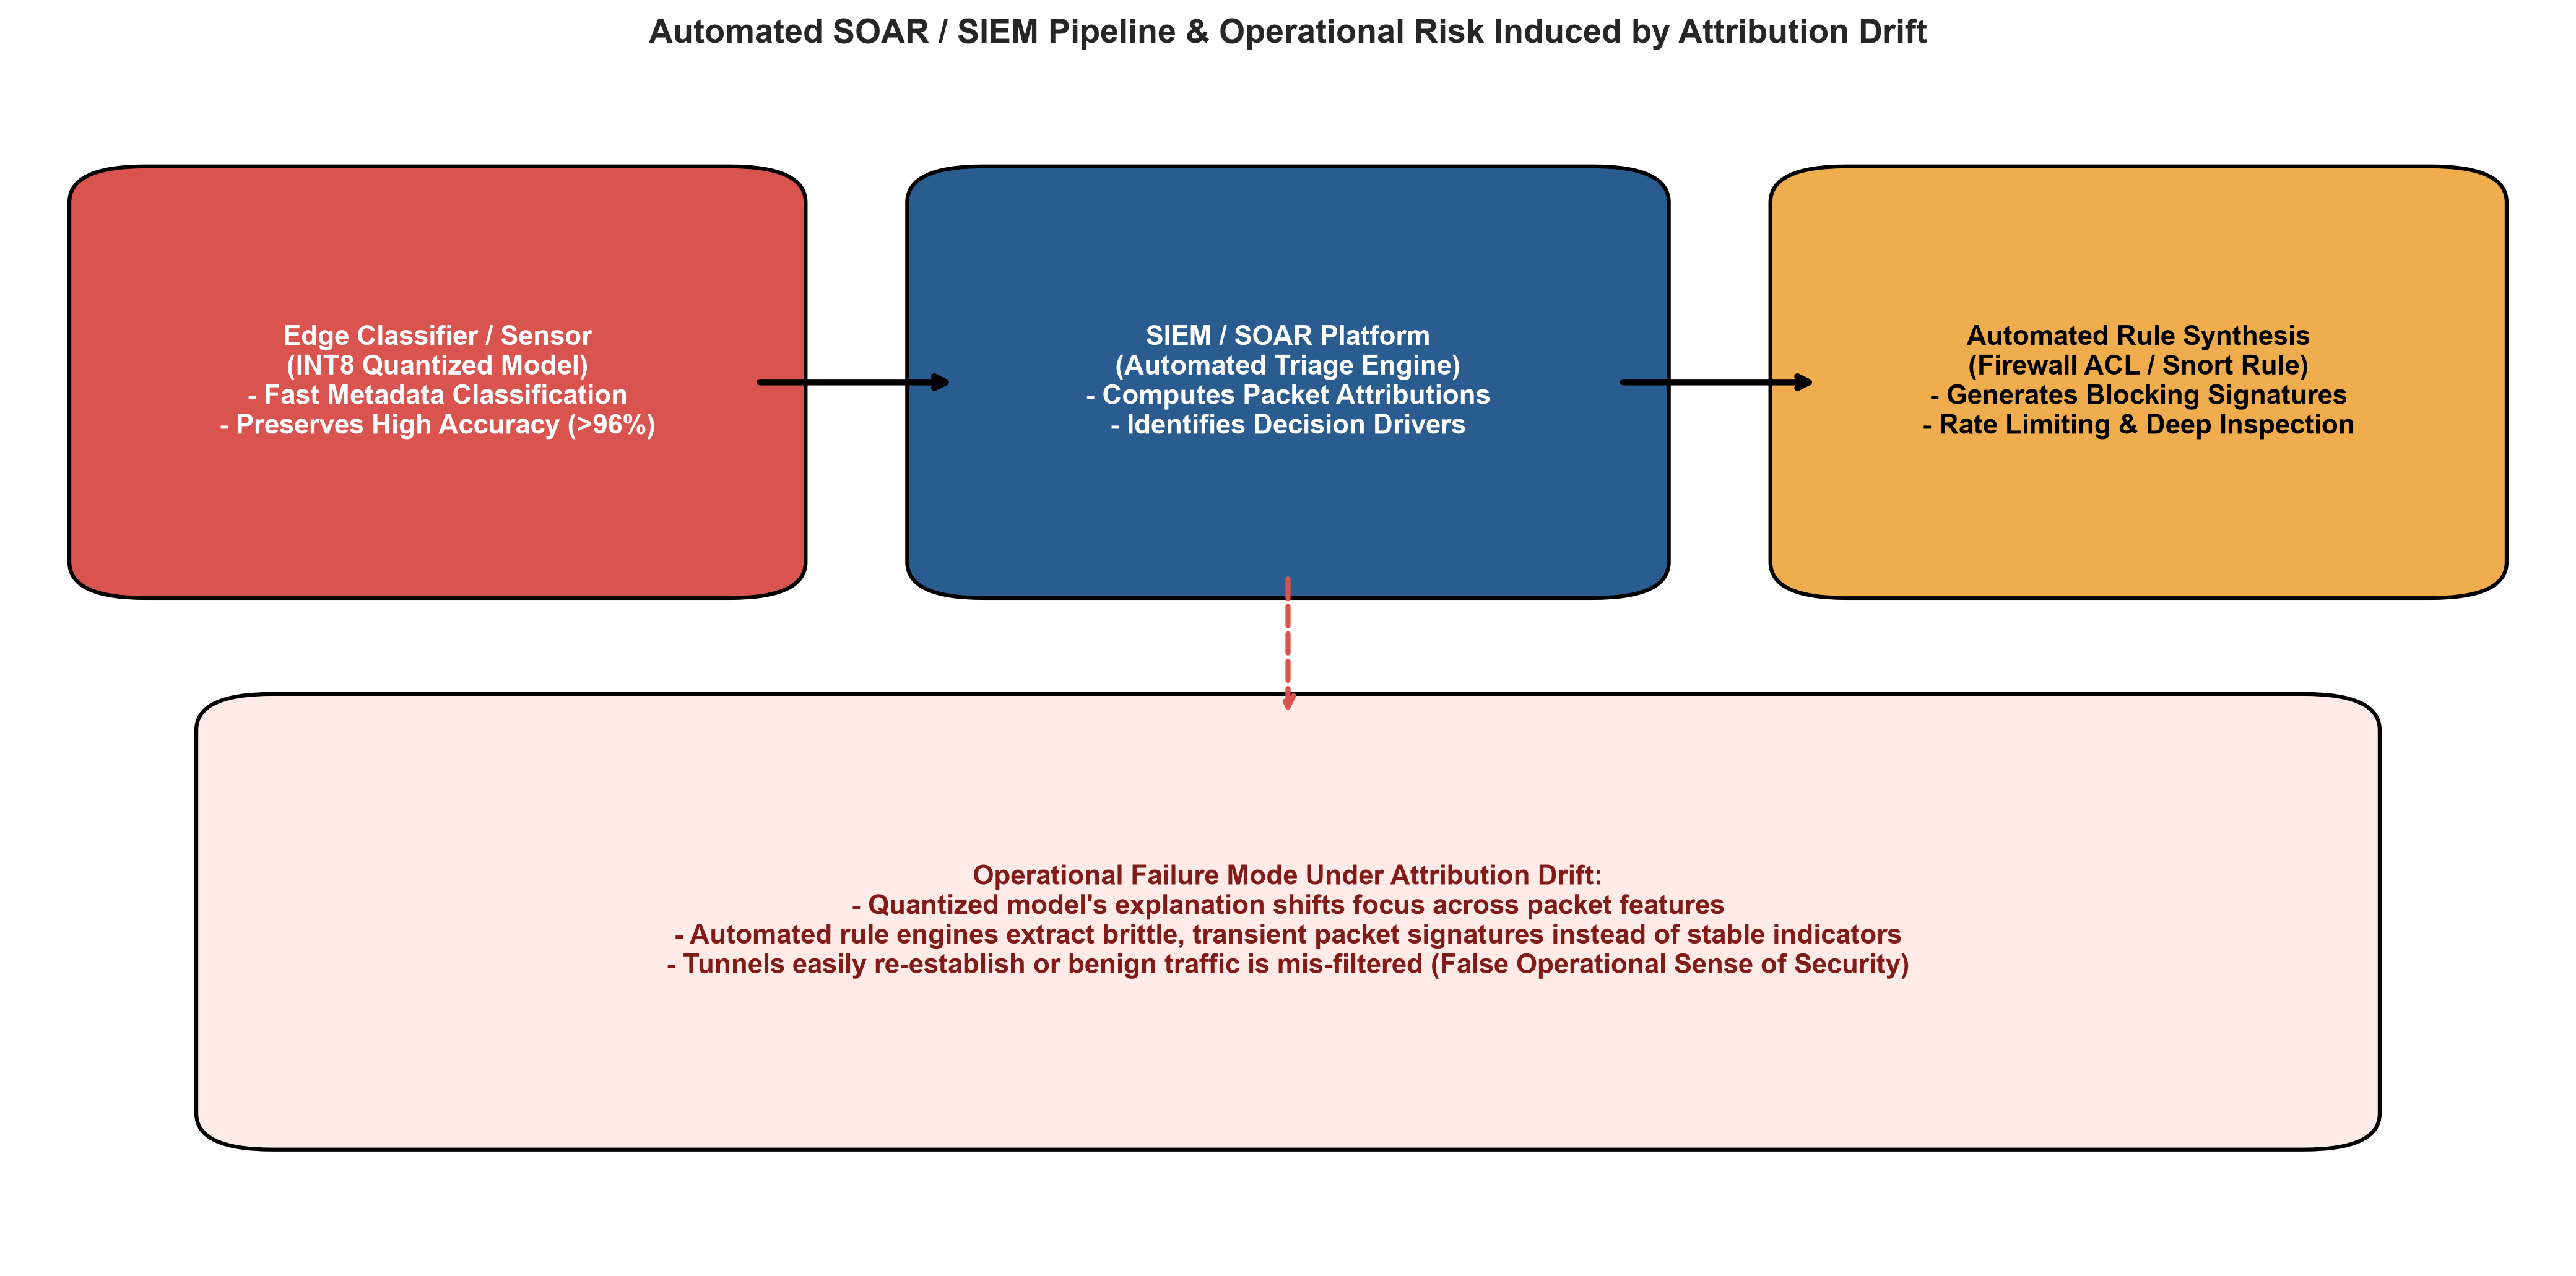
\includegraphics[width=\textwidth]{figures/figure_13_soar_siem_pipeline_and_threat_model.png}
\caption{SOAR/SIEM Alert Suppression Pipeline and Threat Model under Fixed-Point Quantization Saturation. (a) Integer affine transformation truncating pre-sigmoid logits at $z_{\max} = +1.01405$, enforcing an absolute probability ceiling of $p_{\max} = 0.733812$. (b) Downstream triage failure where conservative NIDS thresholds ($\tau = 0.900$) cause 100\% VPN alert suppression. (c) Adversarial exploitation and queue starvation: zero-variance score clamping forces SIEM engines into FIFO fallback, blinding human analysts to targeted exfiltration channels.}
\label{fig:soar_threat_model}
\end{figure*}

This clamping behavior introduces operational failure modes into modern Security Orchestration, Automation, and Response (SOAR) and Security Information and Event Management (SIEM) pipelines \cite{b27}, as illustrated in Fig.~\ref{fig:soar_threat_model}:
\begin{enumerate}
    \item \textbf{Dynamic Alert Prioritization and Queue Sorting:} SOAR playbooks rank incoming security incidents by assigning high-confidence alerts ($p > 0.95$) to automated containment actions (e.g., dynamic firewall access-list blacklisting, active TCP reset injection) while routing intermediate-confidence alerts ($0.65 \le p \le 0.85$) to human security analysts for manual verification. Clamping $98.11\%$ of all positive detections to an identical value of $0.733812$ collapses alert score variance to zero. Automated sorting algorithms cannot distinguish high-certainty malicious tunneling from marginal protocol anomalies. Priority queues lose all discriminatory power.
    \item \textbf{Alert Flooding and Denial-of-Triage:} When thousands of concurrent network flows generate alerts with identical confidence values, incident queuing engines resort to non-deterministic first-in-first-out (FIFO) scheduling. Adversaries can exploit this vulnerability intentionally. An adversary can exploit this behavior by injecting bursts of background tunneling traffic to overwhelm human analysts with undifferentiated alerts, blinding the SOC to targeted exfiltration channels \cite{b28}, \cite{b25}. Target traffic hides inside the clamped cohort.
    \item \textbf{Forensic Explanation Coupling:} Because $98.11\%$ of true positive flows share the exact same clamped logit, automated playbooks cannot correlate confidence drops with specific packet anomalies. Downstream explanation generation engines lose their calibrated reference anchors, propagating spurious packet length rules into perimeter filtering tables \cite{b29}, \cite{b26}. Explanations decouple from actual risk levels.
\end{enumerate}

\subsection{Microarchitectural Profiling and ARM64 Edge Duality}
Deploying deep traffic classifiers to edge hardware involves a trade-off between streaming latency and micro-batched throughput. Hardware constraints dictate operational boundaries. We profiled inference execution on 64-bit ARM64 architecture (Apple Silicon ARM64 running macOS 15.1, executing via PyTorch's native QNNPACK fixed-point runtime engine) to evaluate how fixed-point quantization interacts with hardware execution pipelines.

Our benchmarks uncover an execution duality governed by batch concurrency:
\begin{itemize}
    \item \textbf{Streaming Single-Flow Latency ($BS = 1$):} Under strict streaming conditions where individual network packets or completed flow records are processed sequentially upon arrival ($BS = 1$), INT8-PTQ requires a median latency of $0.255\text{ ms}$ per flow ($3,797\text{ flows/s}$), compared to $0.267\text{ ms}$ ($3,439\text{ flows/s}$) for the uncompressed FP32 baseline. This represents a modest $1.05\times$ latency speedup ($1.10\times$ for INT8-QAT at $0.242\text{ ms}$), with single-flow execution remaining heavily framework-bound. In single-instance execution, total wall-clock latency is dominated by Python runtime interpreter overheads, C++ TorchScript wrapper indirection, dynamic memory allocations, and tensor packing routines. The actual arithmetic execution of the 44,129 model parameters occupies only a minor fraction of the total execution budget. Because the instruction pipeline cannot be filled with vector operations, the arithmetic efficiency of fixed-point integer execution is completely masked by framework indirection. Vector registers sit idle.
    \item \textbf{Micro-Batched Throughput ($BS = 64$):} When incoming flows are accumulated into bounded micro-batches ($BS = 64$), INT8-PTQ achieves a throughput of $76,265\text{ flows/s}$ (median latency $0.764\text{ ms}$), compared to $6,387\text{ flows/s}$ (median latency $9.503\text{ ms}$) for the FP32 baseline. This delivers an $11.94\times$ throughput acceleration ($12.44\times$ median latency speedup; and $12.77\times$ throughput speedup for INT8-QAT at $81,552\text{ flows/s}$). Parallelism transforms execution speed.
\end{itemize}

This $\approx 12\times$ throughput acceleration stems from two microarchitectural mechanisms:
\begin{enumerate}
    \item \textbf{ARM NEON SIMD Vector Parallelism:} On ARMv8-A architectures, 32-bit floating-point multiply-accumulate operations execute over 128-bit NEON registers processing four parallel 32-bit floats per instruction cycle. In contrast, 8-bit integer dot products map directly to specialized vector instructions (e.g., `SDOT'/`UDOT' dot-product instructions on ARMv8.2-A, or vectorized 8-bit integer dot-product pipelines within the ARM NEON architecture). These instructions execute four 8-bit integer multiplications and accumulate the results into a 32-bit destination register within a single vector execution cycle. Micro-batching provides sufficient data concurrency to saturate the NEON execution pipelines, executing four times as many arithmetic operations per cycle compared to floating-point execution. Instruction pipelines remain fully saturated.
    \item \textbf{Cache Hierarchy Residency and Memory Bandwidth:} The entire INT8-PTQ serialized model checkpoint occupies only $51.81\text{ KB}$ of storage, down from $184.2\text{ KB}$ for FP32. On ARM64 architectures, typical L1 data caches allocate $64\text{ KB}$ per core. The complete $51.77\text{ KB}$ INT8 model fits entirely within the per-core cache hierarchy, with convolutional weight buffers residing directly in fast SRAM cache lines. In contrast, the uncompressed $184.24\text{ KB}$ FP32 baseline and its expanded intermediate activation buffers exceed L1 capacity and repeatedly contend for higher-level cache lines, causing eviction cycles and forcing memory stalls over the system bus. Memory stalls vanish. Because fixed-point quantization keeps the entire parameter set resident in fast on-chip SRAM, execution becomes compute-bound rather than memory-bandwidth-bound.
\end{enumerate}

Edge security designs must not implement naive synchronous single-flow inspection. Per-packet dispatch wastes computational resources. Perimeter security gateways must implement bounded temporal micro-batching queues (e.g., buffering flows over a 5 to 10 ms window to assemble batches of $BS = 16$ to $64$) to unlock the full $11.94\times$ NEON SIMD throughput acceleration without compromising streaming latency requirements. Micro-batching bridges the gap between latency and throughput.

\subsection{Regulatory Compliance Mandates and Forensic Auditability}
Deploying machine learning models in automated cybersecurity infrastructure is increasingly governed by international legal frameworks and risk management standards. Legal compliance requires verifiable auditability. Attribution drift creates a direct compliance exposure: models that maintain certified predictive accuracy can introduce significant compliance and defensibility challenges under statutory explainability and oversight frameworks post-quantization. Post-hoc rationales cannot be taken for granted. As codified in the Regulatory Compliance Audit Matrix (Fig.~\ref{fig:regulatory_compliance_matrix}), three frameworks govern edge NIDS deployments:

\begin{figure}[htbp]
\centering
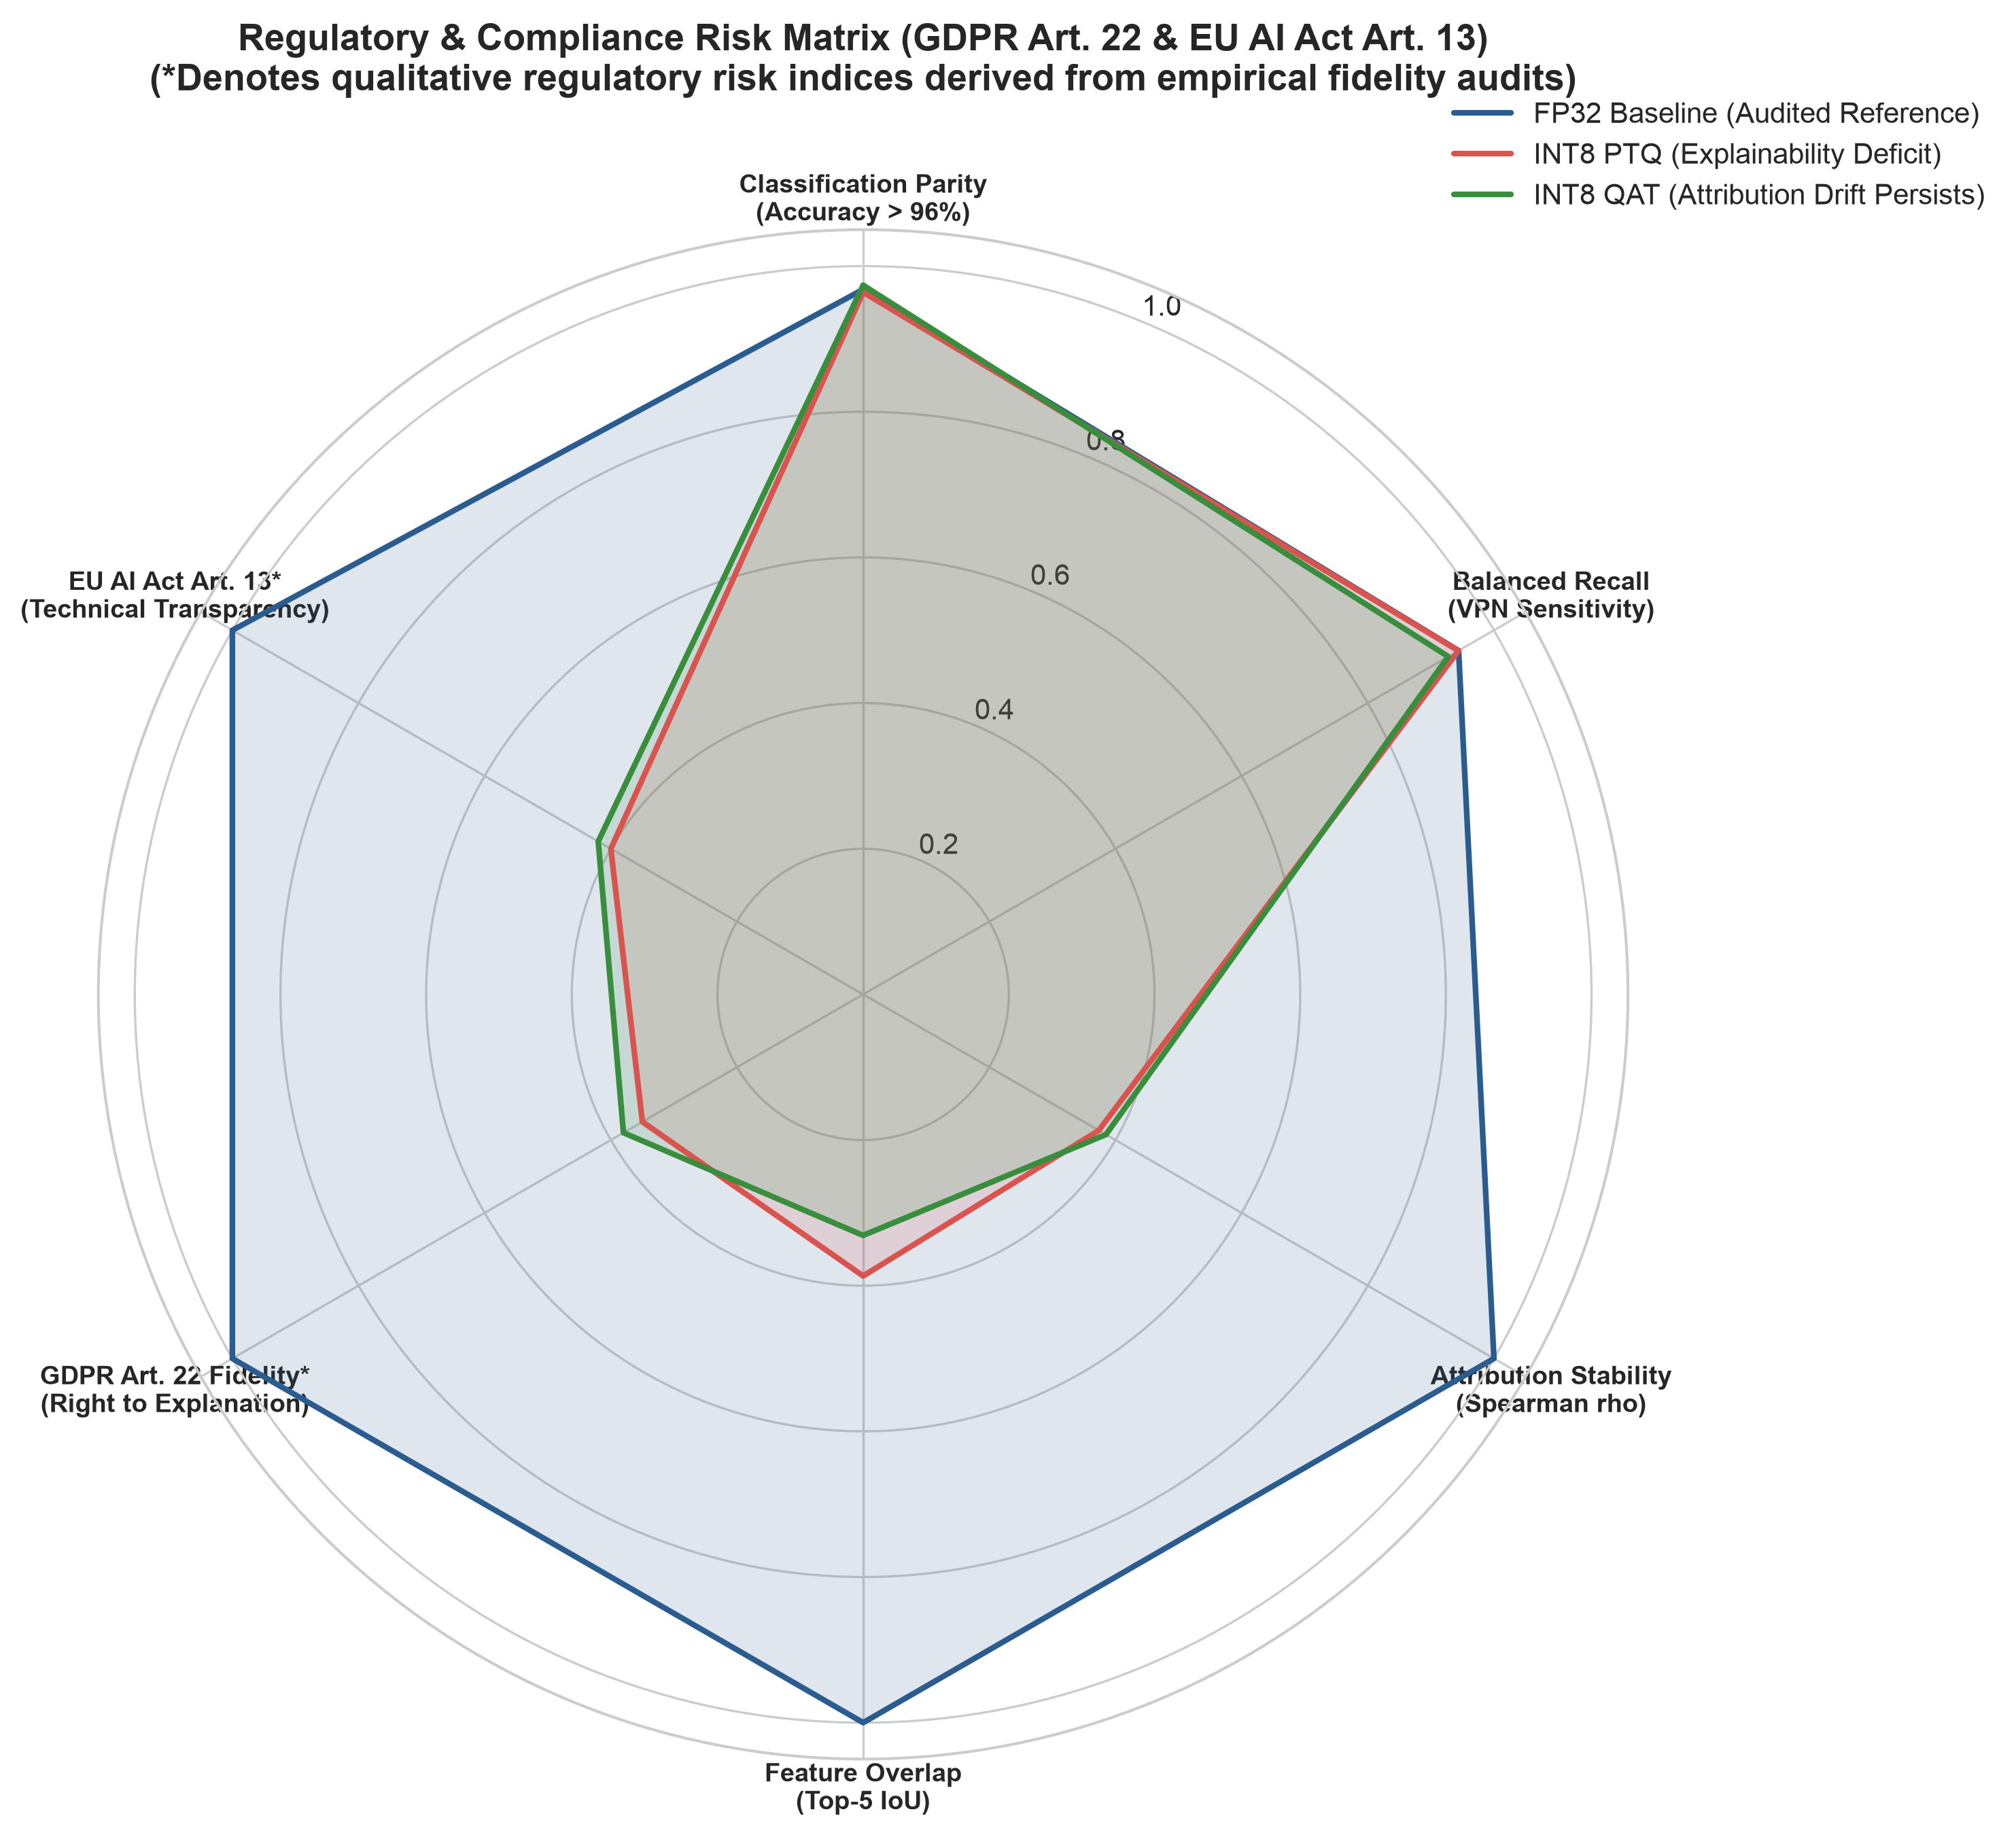
\includegraphics[width=\columnwidth]{figures/figure_14_regulatory_compliance_spider_matrix.png}
\caption{Regulatory Compliance Audit Matrix across EU AI Act, GDPR, and NIST AI RMF 1.0. Fixed-point INT8-PTQ maintains compliance across transparency, oversight, and validity dimensions, whereas INT8-QAT introduces substantial compliance and defensibility risks across explainability, human oversight, and metric reliability dimensions due to directional attribution collapse ($S_c = 0.4830$ overall, $0.1665$ on VPN flows) and confidence clamping ($p_{\max} = 0.733812$).}
\label{fig:regulatory_compliance_matrix}
\end{figure}

\begin{enumerate}
    \item \textbf{EU Artificial Intelligence Act (Regulation EU 2024/1689) \cite{b8}:} Under Article 13 (``Transparency and provision of information to deployers''), high-risk AI systems deployed within critical infrastructure (Annex III) must be developed to enable deployers to interpret system outputs and act appropriately. Deploying an INT8-QAT model that achieves VPN-class $F_1 = 0.7762$ while directional attribution alignment drops to $S_c = 0.4830$ overall (and collapses to $S_c = 0.1665$ on VPN flows) creates serious compliance and defensibility risks under Article 13. If an enterprise attempts to satisfy transparency requirements using explanations generated from the pre-deployment FP32 model, those explanations misrepresent the actual decision logic executed by the compiled edge binary. In parallel, Article 14 (``Human oversight'') mandates that operational interfaces enable natural persons to oversee execution, prevent errors, and intervene. When integer clamping forces $98.11\%$ of positive detections to an identical score ($p_{\max} = 0.733812$), security analysts are deprived of confidence-based triage signals, severely impairing the technical fidelity required for meaningful human oversight and prioritized incident response.
    \item \textbf{General Data Protection Regulation (GDPR, Regulation EU 2016/679) \cite{b7}:} Article 22 (``Automated individual decision-making, including profiling'') restricts decisions based solely on automated processing producing legal or similarly substantial consequences on natural persons, guaranteeing data subjects the right to obtain human intervention and meaningful explanations (Recital 71). Automated network enforcement triggers strict legal scrutiny. When traffic classifiers enforce automated network quarantine, bandwidth throttling, or zero-trust access revocation, automated actions trigger Article 22 scrutiny. If automated traffic classifiers enforce automated policy actions (e.g., zero-trust quarantine or access revocation), explanations derived from a pre-compilation FP32 model fail to provide an accurate factual account of the automated decision. Our demonstration that directional attribution alignment collapses to $S_c = 0.1665$ (with $\text{IoU}_5 = 0.9350$) on VPN flows reveals that post-hoc explanations can attribute decisions to features that the deployed integer model discounted, creating significant evidentiary and defensibility vulnerabilities during administrative reviews or forensic audits.
    \item \textbf{NIST AI Risk Management Framework (AI RMF 1.0) \cite{b9}:} NIST AI RMF 1.0 establishes core trustworthiness characteristics across the system lifecycle, focusing on \textit{Validity \& Reliability} (Section 1.1) and \textit{Explainability \& Interpretability} (Section 1.3). Compression must preserve model trustworthiness. The framework dictates that AI systems must remain valid under operational deployment conditions, and that compression must not introduce uncharacterized behavioral divergences. Deploying quantized classifiers without verifying post-compression attribution stability departs from core NIST AI RMF recommendations under the Govern, Map, and Measure functions, which emphasize that AI systems must maintain characterized validity under operational deployment conditions.
\end{enumerate}

These statutory requirements demonstrate that post-hoc explanations cannot be treated as static assets certified prior to compilation. Explanations evolve across compilation stages. Explainability must be audited as a dynamic, deployment-dependent artifact directly on physical integer execution runtimes. Runtime verification is essential for high-assurance edge security deployments.

\subsection{Clustered Statistical Inference and Simpson's Paradox}
A structural vulnerability in published network traffic classification research is the uncritical application of independent and identically distributed (i.i.d.) statistical assumptions to non-independent network flows \cite{b25}, \cite{b26}. Real-world traffic violates independence. In physical networks, traffic flows captured during the same measurement session share common operating system network stacks, congestion control state machines, transmission control protocol (TCP) window scaling configurations, and physical link jitter \cite{b1}, \cite{b24}. Treating individual flows as statistically independent observations commits a pseudo-replication fallacy that invalidates standard hypothesis tests. Common network stacks induce shared error structures.

Our held-out evaluation test partition contains $N = 49,251$ bidirectional flows partitioned across $K = 16$ canonical capture sessions. If we evaluate pre-sigmoid logit shifts between the uncompressed FP32 baseline and INT8-PTQ ($\Delta z = z_{\text{PTQ}} - z_{\text{FP32}}$) using an unclustered paired $t$-test across all $49,251$ flows yields an extreme test statistic of $t = -38.93$ ($p < 10^{-300}$), which superficially appears to prove systematic negative logit depression.
Naive unclustered tests produce false certainty.

Hierarchical decomposition across the $K = 16$ session clusters reveals that this conclusion is an artifact of sample size inflation and session concentration. The apparent aggregate shift is illusory. As documented in Table~\ref{tab:session_shifts}, the test partition exhibits extreme volume skew: a single capture session, \texttt{skype\_audio3}, contains $39,179$ flows, representing $79.55\%$ of the entire evaluation dataset. Within that dominant Skype trace, PTQ causes a negative mean logit shift of $\overline{\Delta z} = -0.1164$ ($\sigma = 0.2303$). In contrast, 13 out of the 16 canonical sessions ($81.25\%$) exhibit strictly positive logit shifts, ranging from $+0.1037$ in \texttt{icqchat1} up to $+0.5262$ in \texttt{netflix2}. Only three sessions exhibit negative shifts: \texttt{skype\_audio3} ($-0.1164$), \texttt{email1} ($-0.0543$), and \texttt{vpn\_bittorrent} ($-0.7204$). Session majorities point in the opposite direction.

To formalize this disparity, we define two distinct statistical estimands:
\begin{align}
\theta_A &= \frac{\sum_{k=1}^K \sum_{i=1}^{n_k} \Delta z_{k,i}}{\sum_{k=1}^K n_k} = -0.0778, \label{eq:estimand_a_eval} \\
\theta_B &= \frac{1}{K} \sum_{k=1}^K \overline{\Delta z}_k = +0.2270. \label{eq:estimand_b_eval}
\end{align}
Estimand A evaluates the micro-averaged, flow-weighted pooled mean. It answers an operational query: what is the net logit displacement across all flows captured in this specific network trace? Estimand B evaluates the macro-averaged session mean. It answers an inductive query: what is the expected logit shift when deploying the quantized model to an unseen, independent network session? The two estimands answer distinct operational questions.

This divergence constitutes an empirical manifestation of Simpson's Paradox: the aggregate pooled flow effect ($\theta_A = -0.0778$) is strictly negative, directly reversing the positive effect present across $81.25\%$ of the underlying independent sub-populations ($\theta_B = +0.2270$). Aggregation reverses the underlying trend.

We computed confidence intervals using cluster bootstrap resampling with replacement across the $K = 16$ canonical sessions ($B = 2,000$ iterations, seed 42):
\begin{itemize}
    \item For Estimand A, the cluster bootstrap produces a $95\%$ confidence interval of $[-0.1124, +0.3275]$. Because this interval spans zero, the apparent negative logit shift is not statistically distinguishable from zero once session clustering is recognized. The zero-crossing negates the naive $t$-test.
    \item For Estimand B, the cluster bootstrap produces a $95\%$ confidence interval of $[+0.0630, +0.3554]$. This interval is strictly positive and bounded away from zero. Unseen sessions shift positive.
\end{itemize}

The empirical replicate distribution of Estimand A is bimodal rather than normal. Session imbalance generates two competing modes. The probability of selecting the dominant session \texttt{skype\_audio3} at least once in a cluster bootstrap draw of $K = 16$ clusters sampled with replacement evaluates, as derived in (\ref{eq:skype_prob}), to $P(\texttt{skype\_audio3} \in \text{sample}) = 1 - (1 - 1/K)^K \approx 64.39\%$.
In the $64.39\%$ of bootstrap draws containing \texttt{skype\_audio3}, its $39,179$ flows anchor the weighted average, concentrating replicate values between $-0.11$ and $-0.07$. In the remaining $35.61\%$ of bootstrap draws where \texttt{skype\_audio3} is omitted, the remaining 15 sessions govern the calculation. Because 13 of those 15 sessions have positive means, the replicate average shifts upward into a secondary mode centered between $+0.05$ and $+0.35$. Dominant clusters distort statistical estimates.

A leave-one-group-out (LOGO) sensitivity analysis confirms this concentration: removing \texttt{skype\_audio3} flips the pooled flow-weighted mean from $-0.0778$ to $+0.0720$. Removing any of the other 15 sessions leaves the pooled mean unchanged between $-0.0725$ and $-0.0955$. The unclustered i.i.d. assumption deflates standard errors by a factor of approximately $56\times$, converting an ecological artifact of one capture file into false statistical certainty. Standard error deflation conceals real variance. Clustered statistical inference is indispensable for evaluating network traffic classifiers. Cluster-aware methodology is essential.

\subsection{Threats to Validity and Practical Limitations}
To ensure methodological transparency, we delineate twelve specific threats to validity and experimental limitations:
\begin{enumerate}
    \item \textbf{Model Architectural Scope (1D-CNN Focus):} Our investigation evaluates a lightweight 1D-CNN architecture (3 convolutional blocks, batch normalization, global pooling, 44,129 parameters) engineered specifically for low-power edge gateways \cite{b2}, \cite{b3}. Edge hardware imposes strict parameter limits. While representative of embedded NIDS classifiers, these findings may not directly generalize to deep sequence architectures such as datagram Transformers (e.g., WF-Transformer \cite{b30}), Recurrent Neural Networks (LSTM/GRU), or Spatio-Temporal Graph Neural Networks without dedicated empirical replication.
    \item \textbf{Benchmark Dataset Specificity (CIC ISCX 2016):} Experiments were conducted on the Canadian Institute for Cybersecurity ISCX VPN-NonVPN 2016 dataset \cite{b1}. Data age represents an unavoidable boundary. Although this benchmark remains the canonical public standard for encrypted traffic classification, its traffic traces reflect network topologies, operating systems, and application behaviors from 2016. Modern zero-RTT handshakes, TLS 1.3 encrypted client hellos (ECH), and post-quantum cryptographic encapsulations are not represented in this corpus.
    \item \textbf{Finite Session Cluster Count ($K = 16$):} Although session-level clustering successfully exposed Simpson's Paradox and standard error deflation, our held-out test partition contained exactly $K = 16$ canonical capture sessions. Cluster counts limit parametric modeling options. While sufficient for non-parametric cluster bootstrapping, 16 clusters limit the degrees of freedom available for high-dimensional generalized estimating equations (GEE) or mixed-effects regression modeling.
    \item \textbf{Minority Class Session Sparsity ($K_{\text{vpn}} = 3$):} Within the 16 test sessions, only three sessions correspond to true VPN traffic (\texttt{vpn\_hangouts\_audio2}, \texttt{vpn\_bittorrent}, and an encrypted browsing trace). Obfuscated tunnels remain inherently sparse. This sparsity reflects the real-world operational imbalance between background traffic and obfuscated tunnels, but it constrains empirical variance estimation across independent VPN implementations.
    \item \textbf{Explainability Audit Cohort Bounds ($N = 100$):} Detailed KernelSHAP attribution audits were conducted over a stratified cohort of 100 flows (50 VPN, 50 Non-VPN). Coalition sampling incurs immense computational cost. This sample size was bounded by computational complexity: evaluating 150 coalitions against 50 background reference flows across 128 input dimensions requires 750,000 forward model passes per flow, rendering full-dataset attribution audits computationally intractable on unaccelerated CPU clusters.
    \item \textbf{Stationary, Non-Adversarial Traffic Assumptions:} Our study evaluated models under stationary network conditions. Real-world adversaries actively manipulate traffic patterns. We did not subject the quantized classifiers to active adversarial evasion attacks, packet padding manipulation, timing jitter injection, or adversarial flow morphing designed to exploit attribution drift \cite{b28}, \cite{b31}.
    \item \textbf{Hardware Platform Specificity (Apple Silicon ARM64 / QNNPACK):} Edge benchmarking was performed on Apple Silicon ARM64 under macOS 15.1 using PyTorch's native QNNPACK runtime engine. While this confirms the microarchitectural behavior of fixed-point kernels on 64-bit ARM architectures, performance profiles, cache residency dynamics, and SIMD speedups may vary on embedded low-power appliances (e.g., Raspberry Pi Cortex-A72), microcontrollers, or dedicated Neural Processing Units (NPUs).
    \item \textbf{Background Reference Distribution Sensitivity:} KernelSHAP estimates feature importance by marginalizing missing features against an empirical background dataset ($M = 50$ training flows) \cite{b32}, \cite{b29}. Baseline selection shifts reference coordinate frames. Alternative baseline selections—such as all-zero references, maximum entropy uniform noise, or domain-specific medoid flows—can shift the zero-point of the attribution space.
    \item \textbf{Fixed Sequence Truncation Horizon ($L = 64$):} Input tensors were bounded to the initial 64 bidirectional packets of each flow, right-zero-padded where $L < 64$. Truncation ignores long-term flow evolution. While the initial 64 packets capture protocol handshakes and TLS parameter negotiations, long-lived persistent tunnels spanning hours or millions of packets are classified exclusively on their initial establishment burst.
    \item \textbf{Feature Abstraction Bounds (2-Channel Metadata):} Inputs were featurized strictly as 2-channel tensors of normalized signed packet lengths and log-scaled inter-arrival times to adhere to Deep Packet Inspection (DPI) non-inspection privacy boundaries \cite{b7}, \cite{b8}. Privacy boundaries restrict feature engineering choices. This abstraction purposefully omits TCP flags, window advertisements, TLS extension headers, and flow-level burstiness statistics.
    \item \textbf{Static Integer Quantization Granularity (Uniform INT8):} Evaluations evaluated uniform affine and symmetric 8-bit integer quantization (INT8 via QNNPACK). Quantization schemes continue to evolve. We did not evaluate non-uniform quantization grids, learned step-size quantization (LSQ), extreme low-bit regimes (INT4, 1-bit binarization), or emerging 8-bit floating-point formats (FP8 E4M3/E5M2).
    \item \textbf{Explainer Algorithmic Constraints under Non-Differentiability:} Because compiled INT8 execution engines execute step functions whose analytical gradients are zero almost everywhere, explainability audits were restricted to perturbation-based surrogates (KernelSHAP). Non-differentiable kernels block analytical gradients. Path-integral gradient methods (Integrated Gradients) were evaluated via floating-point surrogate graphs, which cannot execute directly on pure integer hardware graphs without runtime emulation \cite{b29}, \cite{b33}.
\end{enumerate}

\subsection{Defensive Engineering Protocol for Production Edge Security}
To translate these scientific findings into operational practice, we codify a defensive engineering protocol for deploying quantized deep network traffic classifiers in enterprise firewalls, residential routers, and edge security appliances:

\begin{enumerate}
    \item \textbf{Rule 1: Post-Deployment Threshold Re-Calibration and Saturation Auditing:} Security engineers must never deploy a quantized classifier using default floating-point decision thresholds ($\tau = 0.500$ or $\tau = 0.900$) without empirical calibration against compiled execution kernels. Default settings cause silent operational failure. Prior to perimeter deployment, engineers must analytically compute the dequantization logit ceiling $z_{\max} = s \cdot (q_{\max} - zp)$ and the corresponding probability ceiling $p_{\max} = \sigma(z_{\max})$. The operational threshold must be recalibrated on hardware-in-the-loop validation data to satisfy $\tau_{\text{cal}} \le p_{\max} - 0.05$. In production, monitoring pipelines must actively audit the predicted probability distribution: if more than $10\%$ of positive detections cluster at the exact scalar ceiling $p_{\max}$, the model must be flagged for triage failure, and alert confidence sorting must be suspended in downstream SOAR playbooks. Alert sorting requires verified score diversity.
    \item \textbf{Rule 2: Dual-Explainer Verification and Noise-Floor Boundary Validation:} Organizations must never assume that an explainability pipeline certified on an FP32 baseline transfers faithfully to a quantized edge deployment. Explanations do not survive compilation intact. Deployers must establish an empirical Explainer Noise Floor by running multi-seed evaluations of the perturbation explainer on the uncompressed baseline. Deployed edge artifacts must undergo formal drift auditing over a stratified verification cohort: directional alignment must satisfy $S_c \ge S_{c, \text{floor}} - \sigma_{\text{floor}}$ ($S_c \ge 0.82$), and feature selection must satisfy $\text{Top-5 IoU} \ge 0.90$. If an INT8-QAT model exhibits representational collapse ($S_c < 0.70$, as observed on VPN traffic), the system must be rejected for operational deployment, and static INT8-PTQ must be selected as the certified deployment artifact. In high-assurance environments, perturbation-based attributions must be cross-validated against path-integral Integrated Gradients surrogates to confirm structural consensus. Dual explainers prevent single-tool verification blindspots.
    \item \textbf{Rule 3: Streamlined Micro-Batching Architecture for Edge Ingestion:} Perimeter NIDS architectures must discard naive synchronous single-flow ($BS = 1$) inference pipelines. Synchronous dispatch squanders processor capabilities. Because Python runtime indirection and tensor wrapping negate arithmetic acceleration at $BS = 1$ ($1.05\times$ speedup), edge ingestion engines must implement bounded micro-batch queues. By buffering incoming flow records over a $5\text{ to }10\text{ ms}$ temporal window, the ingestion engine constructs micro-batches of $BS = 16\text{ to }64$. This queue architecture saturates 64-bit and 128-bit ARM NEON SIMD vector dot-product pipelines, unlocking an $11.94\times$ throughput acceleration ($76,265\text{ flows/s}$ under PTQ, and $81,552\text{ flows/s}$ under QAT). It also maintains complete model parameter residency within on-chip cache ($51.77\text{ KB}$ footprint), eliminating DRAM bus bottlenecks while strictly adhering to real-time microsecond SLA deadlines. Cache residency ensures deterministic execution latency.
    \item \textbf{Rule 4: Clustered Session-Aware Drift Auditing and Stratification:} Quality assurance pipelines must systematically ban unclustered i.i.d. evaluation metrics. Independent assumptions yield invalid confidence bounds. Before approving any compressed model for production rollout, verification suites must group evaluation network traces into their constituent capture sessions or physical host origins ($K \ge 16$), compute and report both statistical estimands (the pooled micro-average $\theta_A$ and the session macro-average $\theta_B$), and execute cluster bootstrap resampling ($B \ge 2,000$ iterations) across session clusters to construct valid confidence intervals. If the bootstrap distribution exhibits bimodality or the confidence interval for the primary deployment estimand spans zero, the model must be audited for single-session concentration bias before production authorization. Clustered auditing certifies true inductive generalization.
\end{enumerate}


\section{Conclusion}
This study investigated the impact of fixed-point integer quantization on feature attribution stability in deep encrypted traffic classifiers deployed at the network edge. Using a 1D-CNN trained on the ISCX VPN-NonVPN benchmark, we demonstrated that macroscopic classification parity does not guarantee explainability preservation. While static Post-Training Quantization (INT8-PTQ) achieved a $3.56\times$ model compression ratio with near-perfect attribution fidelity ($S_c = 0.9918$, Top-5 IoU = $0.9786$) well inside the empirical explainer noise floor ($S_c = 0.9676 \pm 0.1450$), Quantization-Aware Training (INT8-QAT) induced severe attribution restructuring ($S_c = 0.4830$ across the full cohort, collapsing to $S_c = 0.1665$ on minority VPN traffic). Through an unquantized fine-tuning control (FP32-FT), we established that this restructuring is driven by stochastic gradient descent navigating an overparameterized empirical loss surface ($TV = 0.1219, p = 4.66 \times 10^{-9}$), but discrete integer quantization constraints and STE approximations drive severe additional representational collapse on minority VPN flows ($S_c = 0.1665, W = 1146.0, p = 2.12 \times 10^{-6}$ vs. FP32-FT).

Beyond attribution drift, we characterized an operational deployment hazard: affine dequantization in compiled edge execution engines (QNNPACK) enforces an absolute probability ceiling ($p_{\max} = 0.733812$), clamping $98.11\%$ of true VPN detections and causing complete classification blackout under default decision thresholds. While micro-batched execution ($BS=64$) unlocks an $11.94\times$ throughput acceleration on ARM64 hardware through SIMD vectorization and cache residency, single-flow streaming ($BS=1$) yields negligible gains due to runtime framework dispatch overhead. Finally, session-clustered bootstrapping exposed an empirical instance of Simpson's Paradox, demonstrating that unclustered flow-level statistical evaluations underestimate variance by up to $56\times$. These findings establish that model compression and explainability auditing cannot be treated as independent lifecycle phases. Production edge deployments require hardware-in-the-loop threshold recalibration, multi-seed explainer noise floor boundaries, and session-aware clustered quality assurance.

\begin{thebibliography}{00}
\bibitem{b1} G. Draper-Gil, A. H. Lashkari, M. S. I. Mamun, and A. A. Ghorbani, "Characterization of encrypted traffic through flow interaction," in Proc. 2nd Int. Conf. Inf. Syst. Secur. Privacy (ICISSP), Rome, Italy, 2016, pp. 297–304, doi: 10.5220/0005740704070414.
\bibitem{b2} W. Wang, M. Zhu, J. Wang, X. Zeng, and Z. Yang, "End-to-end encrypted traffic classification with one-dimensional convolution neural networks," in Proc. IEEE Int. Conf. Intell. Secur. Informatics (ISI), Beijing, China, 2017, pp. 43–48, doi: 10.1109/ISI.2017.8004872.
\bibitem{b3} M. Lotfollahi, M. J. Siavoshani, R. S. H. Zadeh, and M. Saberian, "Deep Packet: A novel approach for encrypted traffic classification using deep learning," Soft Computing, vol. 24, no. 3, pp. 1999–2012, Feb. 2020, doi: 10.1007/s00500-019-04030-2.
\bibitem{b4} S. M. Lundberg and S.-I. Lee, "A unified approach to interpreting model predictions," in Adv. Neural Inf. Process. Syst. (NeurIPS), vol. 30, Long Beach, CA, USA, 2017, pp. 4765–4774.
\bibitem{b5} B. Jacob, S. Kligys, B. Chen, M. Zhu, M. Tang, A. Howard, H. Adam, and D. Kalenichenko, "Quantization and training of neural networks for efficient integer-arithmetic-only inference," in Proc. IEEE/CVF Conf. Comput. Vis. Pattern Recognit. (CVPR), Salt Lake City, UT, USA, 2018, pp. 2704–2713, doi: 10.1109/CVPR.2018.00286.
\bibitem{b6} S. Hooker, A. Courville, G. Clark, Y. Dauphin, and A. Frome, "What do compressed deep neural networks forget?," in Adv. Neural Inf. Process. Syst. (NeurIPS), vol. 32, Vancouver, BC, Canada, 2019, pp. 1464–1475.
\bibitem{b7} European Parliament and Council of the European Union, "Regulation (EU) 2016/679 on the protection of natural persons with regard to the processing of personal data (General Data Protection Regulation)," Off. J. Eur. Union, L 119, pp. 1–88, May 2016.
\bibitem{b8} European Parliament and Council of the European Union, "Regulation (EU) 2024/1689 laying down harmonised rules on artificial intelligence (Artificial Intelligence Act)," Off. J. Eur. Union, L 2024/1689, Jul. 2024.
\bibitem{b9} National Institute of Standards and Technology, "Artificial Intelligence Risk Management Framework (AI RMF 1.0)," NIST AI 100-1, Gaithersburg, MD, USA, Jan. 2023, doi: 10.6028/NIST.AI.100-1.
\bibitem{b10} G. Aceto, D. Ciuonzo, A. Montieri, and A. Pescapé, "MIMETIC: Mobile encrypted traffic classification using multimodal deep learning," Computer Networks, vol. 165, p. 106944, Dec. 2019, doi: 10.1016/j.comnet.2019.106944.
\bibitem{b11} C. Liu, L. He, G. Xiong, Z. Cao, and Z. Li, "FS-Net: A flow sequence network for encrypted traffic classification," in Proc. IEEE INFOCOM, Paris, France, 2019, pp. 1171–1179, doi: 10.1109/INFOCOM.2019.8737507.
\bibitem{b12} T. van Ede, R. Bortolameotti, A. Continella, J. Ren, D. J. Dubois, M. Lindorfer, D. Choffnes, M. van Steen, and A. Peter, "FlowPrint: Semi-supervised mobile-app fingerprinting on encrypted network traffic," in Proc. Netw. Distrib. Syst. Secur. Symp. (NDSS), San Diego, CA, USA, 2020, pp. 1–18, doi: 10.14722/ndss.2020.24412.
\bibitem{b13} X. Lin, G. Xiong, G. Gou, Z. Li, J. Shi, and J. Yu, "ET-BERT: A contextualized datagram representation with pre-training transformers for encrypted traffic classification," in Proc. ACM Web Conf. (WWW), Lyon, France, 2022, pp. 633–642, doi: 10.1145/3485447.3512217.
\bibitem{b14} Y. Chen and Y. Wang, "MPAF: Encrypted traffic classification with multi-phase attribute fingerprint," IEEE Trans. Inf. Forensics Security, vol. 19, pp. 7091–7105, 2024, doi: 10.1109/TIFS.2024.3428839.
\bibitem{b15} M. Sarhan, S. Layeghy, and M. Portmann, "Evaluating the explainability of machine learning models for network intrusion detection systems," IEEE Trans. Netw. Service Manag., vol. 20, no. 3, pp. 3496–3509, Sep. 2023, doi: 10.1109/TNSM.2023.3235304.
\bibitem{b16} S. Mali, S. Agarwal, R. Chintawar, and A. K. Cherukuri, "Analyzing encrypted traffic analysis using explainable AI," Annals of Mathematics and Computer Science, vol. 31, pp. 1–22, 2025, doi: 10.56947/amcs.v31.660.
\bibitem{b17} A. Sharma, "XAI-driven encrypted traffic detection and characterization to enhance information security," M.A. thesis, Dept. Elect. Eng. Comput. Sci., York Univ., Toronto, Canada, 2025.
\bibitem{b18} S. Khandaker, "Quant-XAI: Quantifying and mitigating explainability drift under INT8 quantization in edge-deployed visual classification," Research Square Preprint, 2026, doi: 10.21203/rs.3.rs-9179249/v1.
\bibitem{b19} Q. Wang, M. Wang, N. Feldhus, S. Ostermann, Y. Cao, H. Schütze, S. Möller, and V. Schmitt, "Through a compressed lens: Investigating the impact of quantization on factual knowledge recall," in Proc. 6th Workshop on Trustworthy NLP (TrustNLP 2026) @ ACL, 2026, pp. 21–39.
\bibitem{b20} R. Krishnamoorthi, "Quantizing deep convolutional networks for efficient inference: A whitepaper," arXiv preprint arXiv:1806.08342, 2018.
\bibitem{b21} M. Dukhan, "The indirect convolution algorithm," arXiv preprint arXiv:1907.02129, 2019.
\bibitem{b22} Y. Bengio, N. Léonard, and A. Courville, "Estimating or propagating gradients through stochastic neurons for conditional computation," arXiv preprint arXiv:1308.3432, 2013.
\bibitem{b23} M. Sundararajan, A. Taly, and Q. Yan, "Axiomatic attribution for deep networks," in Proc. 34th Int. Conf. Mach. Learn. (ICML), Sydney, Australia, 2017, pp. 3319–3328.
\bibitem{b24} X. Lin, G. Xiong, Y. Hao, X. Xie, and Z. Li, "Respond to change with constancy: Instruction-tuning with LLM for non-I.I.D. network traffic classification," IEEE Trans. Inf. Forensics Security, vol. 20, pp. 5758–5773, 2025, doi: 10.1109/TIFS.2025.3537821.
\bibitem{b25} R. Sommer and V. Paxson, "Outside the closed world: On using machine learning for network intrusion detection," in Proc. IEEE Symp. Secur. Privacy (S\&P), Oakland, CA, USA, 2010, pp. 305–316, doi: 10.1109/SP.2010.25.
\bibitem{b26} D. Arp, E. Quiring, F. Pendlebury, A. Warnecke, F. Pierazzi, C. Wressnegger, R. Cavallaro, and K. Rieck, "Dos and don'ts of machine learning in computer security," in Proc. 31st USENIX Secur. Symp., Boston, MA, USA, 2022, pp. 3971–3988.
\bibitem{b27} C. Islam, M. A. Babar, and S. Nepal, "A multi-vocal review of security orchestration, automation, and response (SOAR)," ACM Comput. Surv., vol. 52, no. 2, pp. 1–35, May 2019, doi: 10.1145/3305271.
\bibitem{b28} Y. Hou, C. Gong, H. Sun, Z. Lu, P. Zhou, and X. Guan, "Evading deep learning-based encrypted traffic classification via flow timing and packet size manipulation," IEEE Trans. Inf. Forensics Security, vol. 18, pp. 5231–5245, 2023, doi: 10.1109/TIFS.2023.3306354.
\bibitem{b29} S. Neupane, J. Ables, W. Anderson, F. Pagan, T. K. A. Nguyen, and S. Rahimi, "Explainable AI for network intrusion detection systems: A comparative study," IEEE Trans. Netw. Service Manag., vol. 21, no. 1, pp. 842–856, Feb. 2024, doi: 10.1109/TNSM.2023.3308801.
\bibitem{b30} Q. Zhou, L. Peng, Z. Qin, Y. He, X. Zhou, and K. Sakurai, "WF-Transformer: Learning temporal features for accurate anonymous traffic identification by using transformer networks," IEEE Trans. Inf. Forensics Security, vol. 19, pp. 2736–2751, 2024, doi: 10.1109/TIFS.2024.3355034.
\bibitem{b31} A.-K. Dombrowski, M. Alber, C. Anders, M. Ackermann, K.-R. Müller, and P. Kessel, "Explanations can be manipulated and geometry is to blame," in Adv. Neural Inf. Process. Syst. (NeurIPS), vol. 32, Vancouver, BC, Canada, 2019, pp. 13589–13600.
\bibitem{b32} M. T. Ribeiro, S. Singh, and C. Guestrin, ""Why should I trust you?": Explaining the predictions of any classifier," in Proc. 22nd ACM SIGKDD Int. Conf. Knowl. Discov. Data Min. (KDD), San Francisco, CA, USA, 2016, pp. 1135–1144, doi: 10.1145/2939672.2939778.
\bibitem{b33} J. Adebayo, J. Gilmer, M. Muelly, I. Goodfellow, M. Hardt, and B. Kim, "Sanity checks for saliency maps," in Adv. Neural Inf. Process. Syst. (NeurIPS), vol. 31, Montreal, QC, Canada, 2018, pp. 9505–9515.
\end{thebibliography}

\end{document}
